\documentclass[12pt,letterpaper,reqno,fleqn]{article}
% openbib, notitlepage, onecolumn,openany,openright,twoside,titlepage,final,oneside,

\usepackage[utf8]{inputenc}
\usepackage{amsmath}
\usepackage{amsfonts}
\usepackage{amssymb}
\usepackage{setspace}
\usepackage[left=1in,
            right=1in,
            top=1in,
            bottom=1in]{geometry}
\usepackage{graphicx}
\usepackage{mathtools}
\usepackage[hidelinks]{hyperref}
\usepackage{natbib}
\usepackage{tocloft}

\graphicspath{{plots/}}

\usepackage{titlesec}
\titleformat*{\section}{\normalsize\bfseries}
\titleformat*{\subsection}{\normalsize\bfseries}
\titleformat*{\subsubsection}{\normalsize\bfseries}
\author{Swapnaneel Nath}
\doublespacing
\begin{document}
\title{Comparing Predictive Performance of GARCH and Stochastic Volatility Models}
\thispagestyle{empty}
\begin{singlespace}
\begin{center}
	{Comparing Predictive Performance of GARCH and Stochastic Volatility Models} \\
	\vspace{0.5in}
	A thesis submitted in partial fulfillment\\
	of the requirements for the degree of\\
	{Master of Science in Statistics and Analytics}\\
	\vspace{0.5in}
	by\\
	\vspace{0.5in}
	{Swapnaneel Nath}\\
	Drury University\\
        Bachelor of Business Administration in Economics, 2017\\
        Drury University \\
	Bachelor of Arts in Mathematics, 2017\\
	\vspace{0.5in}
	August 2023\\
	University of Arkansas\\
	\end{center}
\begin{flushleft}
\vspace{0.75in}
This thesis is approved for recommendation to the Graduate Council.\\

\vspace{0.75in}
\begin{minipage}[b]{0.48\textwidth}
\makebox[\textwidth]{\hrulefill}\\
Giovanni Petris, Ph.D.\\
Thesis Director\\[0.5in]
\makebox[\textwidth]{\hrulefill}\\
Avishek Chakraborty, Ph.D.\\
Committee Member\\[0.5in]
%\makebox[\textwidth]{\hrulefill}\\
%Sean Plummer, Ph.D.\\
%Committee member
\end{minipage}
\hfill
\begin{minipage}[b]{0.48\textwidth}
\makebox[\textwidth]{\hrulefill}\\
Sean Plummer, Ph.D.\\
Committee Member\\[0.5in]
%\makebox[\textwidth]{\hrulefill}\\
%Sean Plummer, Ph.D.\\
\end{minipage}
\end{flushleft}
\end{singlespace}

\newpage
\thispagestyle{empty}
\begin{abstract}
This paper compares the predictive performance of two commonly used financial models, the Generalized Auto-Regressive Conditional Heteroskedasticity (GARCH) model, and the Stochastic Volatility model. Both techniques are used in the finance literature to model returns on an asset; the main difference between the two is that the former holds volatility as deterministic, whereas the latter treats it as a stochastic component.

Three 10-year periods (2006-15, 2008-17, and 2010-19) of returns of the S\&P-500 Index are used to train the two models. The parameter estimation is done using Hamiltonian Monte Carlo. Then, using Sequential Monte Carlo updates, returns for 2016, 2018, and 2020 are predicted, and their performance over different time frames---one month, one quarter, and one year---are compared using sum of squared errors (SSE). In addition, the percentage of observed returns for the three years that are captured between the 2.5 percentile and the 97.5 percentile of the predictions are compared. The results of the two models are practically indistinguishable by both criteria.
\end{abstract}
\thispagestyle{empty}

\newpage
\thispagestyle{empty}
\renewcommand{\abstractname}{Acknowledgements}
\begin{abstract}
I would like to thank my professors and friends for the wonderful time I have had at University of Arkansas. 
Thanks, in particular, to Dr. Giovanni Petris for guiding me over the last year through the process of building this thesis. 
\end{abstract}
\thispagestyle{empty}

\newpage

\thispagestyle{empty}

%\section*{\centering{Table of Contents}}
\addcontentsline{toc}{section}{\protect\numberline{}Contents}
\documentclass[12pt,letterpaper,reqno,fleqn]{article}
% openbib, notitlepage, onecolumn,openany,openright,twoside,titlepage,final,oneside,

\usepackage[utf8]{inputenc}
\usepackage{amsmath}
\usepackage{amsfonts}
\usepackage{amssymb}
\usepackage{setspace}
\usepackage[left=1in,
            right=1in,
            top=1in,
            bottom=1in]{geometry}
\usepackage{graphicx}
\usepackage{mathtools}
\usepackage[hidelinks]{hyperref}
\usepackage{natbib}
\usepackage{tocloft}

\graphicspath{{plots/}}

\usepackage{titlesec}
\titleformat*{\section}{\normalsize\bfseries}
\titleformat*{\subsection}{\normalsize\bfseries}
\titleformat*{\subsubsection}{\normalsize\bfseries}
\author{Swapnaneel Nath}
\doublespacing
\begin{document}
\title{Comparing Predictive Performance of GARCH and Stochastic Volatility Models}
\thispagestyle{empty}
\begin{singlespace}
\begin{center}
	{Comparing Predictive Performance of GARCH and Stochastic Volatility Models} \\
	\vspace{0.5in}
	A thesis submitted in partial fulfillment\\
	of the requirements for the degree of\\
	{Master of Science in Statistics and Analytics}\\
	\vspace{0.5in}
	by\\
	\vspace{0.5in}
	{Swapnaneel Nath}\\
	Drury University\\
        Bachelor of Business Administration in Economics, 2017\\
        Drury University \\
	Bachelor of Arts in Mathematics, 2017\\
	\vspace{0.5in}
	August 2023\\
	University of Arkansas\\
	\end{center}
\begin{flushleft}
\vspace{0.75in}
This thesis is approved for recommendation to the Graduate Council.\\

\vspace{0.75in}
\begin{minipage}[b]{0.48\textwidth}
\makebox[\textwidth]{\hrulefill}\\
Giovanni Petris, Ph.D.\\
Thesis Director\\[0.5in]
\makebox[\textwidth]{\hrulefill}\\
Avishek Chakraborty, Ph.D.\\
Committee Member\\[0.5in]
%\makebox[\textwidth]{\hrulefill}\\
%Sean Plummer, Ph.D.\\
%Committee member
\end{minipage}
\hfill
\begin{minipage}[b]{0.48\textwidth}
\makebox[\textwidth]{\hrulefill}\\
Sean Plummer, Ph.D.\\
Committee Member\\[0.5in]
%\makebox[\textwidth]{\hrulefill}\\
%Sean Plummer, Ph.D.\\
\end{minipage}
\end{flushleft}
\end{singlespace}

\newpage
\thispagestyle{empty}
\begin{abstract}
This paper compares the predictive performance of two commonly used financial models, the Generalized Auto-Regressive Conditional Heteroskedasticity (GARCH) model, and the Stochastic Volatility model. Both techniques are used in the finance literature to model returns on an asset; the main difference between the two is that the former holds volatility as deterministic, whereas the latter treats it as a stochastic component.

Three 10-year periods (2006-15, 2008-17, and 2010-19) of returns of the S\&P-500 Index are used to train the two models. The parameter estimation is done using Hamiltonian Monte Carlo. Then, using Sequential Monte Carlo updates, returns for 2016, 2018, and 2020 are predicted, and their performance over different time frames---one month, one quarter, and one year---are compared using sum of squared errors (SSE). In addition, the percentage of observed returns for the three years that are captured between the 2.5 percentile and the 97.5 percentile of the predictions are compared. The results of the two models are practically indistinguishable by both criteria.
\end{abstract}
\thispagestyle{empty}

\newpage
\thispagestyle{empty}
\renewcommand{\abstractname}{Acknowledgements}
\begin{abstract}
I would like to thank my professors and friends for the wonderful time I have had at University of Arkansas. 
Thanks, in particular, to Dr. Giovanni Petris for guiding me over the last year through the process of building this thesis. 
\end{abstract}
\thispagestyle{empty}

\newpage

\thispagestyle{empty}

%\section*{\centering{Table of Contents}}
\addcontentsline{toc}{section}{\protect\numberline{}Contents}
\documentclass[12pt,letterpaper,reqno,fleqn]{article}
% openbib, notitlepage, onecolumn,openany,openright,twoside,titlepage,final,oneside,

\usepackage[utf8]{inputenc}
\usepackage{amsmath}
\usepackage{amsfonts}
\usepackage{amssymb}
\usepackage{setspace}
\usepackage[left=1in,
            right=1in,
            top=1in,
            bottom=1in]{geometry}
\usepackage{graphicx}
\usepackage{mathtools}
\usepackage[hidelinks]{hyperref}
\usepackage{natbib}
\usepackage{tocloft}

\graphicspath{{plots/}}

\usepackage{titlesec}
\titleformat*{\section}{\normalsize\bfseries}
\titleformat*{\subsection}{\normalsize\bfseries}
\titleformat*{\subsubsection}{\normalsize\bfseries}
\author{Swapnaneel Nath}
\doublespacing
\begin{document}
\title{Comparing Predictive Performance of GARCH and Stochastic Volatility Models}
\thispagestyle{empty}
\begin{singlespace}
\begin{center}
	{Comparing Predictive Performance of GARCH and Stochastic Volatility Models} \\
	\vspace{0.5in}
	A thesis submitted in partial fulfillment\\
	of the requirements for the degree of\\
	{Master of Science in Statistics and Analytics}\\
	\vspace{0.5in}
	by\\
	\vspace{0.5in}
	{Swapnaneel Nath}\\
	Drury University\\
        Bachelor of Business Administration in Economics, 2017\\
        Drury University \\
	Bachelor of Arts in Mathematics, 2017\\
	\vspace{0.5in}
	August 2023\\
	University of Arkansas\\
	\end{center}
\begin{flushleft}
\vspace{0.75in}
This thesis is approved for recommendation to the Graduate Council.\\

\vspace{0.75in}
\begin{minipage}[b]{0.48\textwidth}
\makebox[\textwidth]{\hrulefill}\\
Giovanni Petris, Ph.D.\\
Thesis Director\\[0.5in]
\makebox[\textwidth]{\hrulefill}\\
Avishek Chakraborty, Ph.D.\\
Committee Member\\[0.5in]
%\makebox[\textwidth]{\hrulefill}\\
%Sean Plummer, Ph.D.\\
%Committee member
\end{minipage}
\hfill
\begin{minipage}[b]{0.48\textwidth}
\makebox[\textwidth]{\hrulefill}\\
Sean Plummer, Ph.D.\\
Committee Member\\[0.5in]
%\makebox[\textwidth]{\hrulefill}\\
%Sean Plummer, Ph.D.\\
\end{minipage}
\end{flushleft}
\end{singlespace}

\newpage
\thispagestyle{empty}
\begin{abstract}
This paper compares the predictive performance of two commonly used financial models, the Generalized Auto-Regressive Conditional Heteroskedasticity (GARCH) model, and the Stochastic Volatility model. Both techniques are used in the finance literature to model returns on an asset; the main difference between the two is that the former holds volatility as deterministic, whereas the latter treats it as a stochastic component.

Three 10-year periods (2006-15, 2008-17, and 2010-19) of returns of the S\&P-500 Index are used to train the two models. The parameter estimation is done using Hamiltonian Monte Carlo. Then, using Sequential Monte Carlo updates, returns for 2016, 2018, and 2020 are predicted, and their performance over different time frames---one month, one quarter, and one year---are compared using sum of squared errors (SSE). In addition, the percentage of observed returns for the three years that are captured between the 2.5 percentile and the 97.5 percentile of the predictions are compared. The results of the two models are practically indistinguishable by both criteria.
\end{abstract}
\thispagestyle{empty}

\newpage
\thispagestyle{empty}
\renewcommand{\abstractname}{Acknowledgements}
\begin{abstract}
I would like to thank my professors and friends for the wonderful time I have had at University of Arkansas. 
Thanks, in particular, to Dr. Giovanni Petris for guiding me over the last year through the process of building this thesis. 
\end{abstract}
\thispagestyle{empty}

\newpage

\thispagestyle{empty}

%\section*{\centering{Table of Contents}}
\addcontentsline{toc}{section}{\protect\numberline{}Contents}
\documentclass[12pt,letterpaper,reqno,fleqn]{article}
% openbib, notitlepage, onecolumn,openany,openright,twoside,titlepage,final,oneside,

\usepackage[utf8]{inputenc}
\usepackage{amsmath}
\usepackage{amsfonts}
\usepackage{amssymb}
\usepackage{setspace}
\usepackage[left=1in,
            right=1in,
            top=1in,
            bottom=1in]{geometry}
\usepackage{graphicx}
\usepackage{mathtools}
\usepackage[hidelinks]{hyperref}
\usepackage{natbib}
\usepackage{tocloft}

\graphicspath{{plots/}}

\usepackage{titlesec}
\titleformat*{\section}{\normalsize\bfseries}
\titleformat*{\subsection}{\normalsize\bfseries}
\titleformat*{\subsubsection}{\normalsize\bfseries}
\author{Swapnaneel Nath}
\doublespacing
\begin{document}
\title{Comparing Predictive Performance of GARCH and Stochastic Volatility Models}
\thispagestyle{empty}
\begin{singlespace}
\begin{center}
	{Comparing Predictive Performance of GARCH and Stochastic Volatility Models} \\
	\vspace{0.5in}
	A thesis submitted in partial fulfillment\\
	of the requirements for the degree of\\
	{Master of Science in Statistics and Analytics}\\
	\vspace{0.5in}
	by\\
	\vspace{0.5in}
	{Swapnaneel Nath}\\
	Drury University\\
        Bachelor of Business Administration in Economics, 2017\\
        Drury University \\
	Bachelor of Arts in Mathematics, 2017\\
	\vspace{0.5in}
	August 2023\\
	University of Arkansas\\
	\end{center}
\begin{flushleft}
\vspace{0.75in}
This thesis is approved for recommendation to the Graduate Council.\\

\vspace{0.75in}
\begin{minipage}[b]{0.48\textwidth}
\makebox[\textwidth]{\hrulefill}\\
Giovanni Petris, Ph.D.\\
Thesis Director\\[0.5in]
\makebox[\textwidth]{\hrulefill}\\
Avishek Chakraborty, Ph.D.\\
Committee Member\\[0.5in]
%\makebox[\textwidth]{\hrulefill}\\
%Sean Plummer, Ph.D.\\
%Committee member
\end{minipage}
\hfill
\begin{minipage}[b]{0.48\textwidth}
\makebox[\textwidth]{\hrulefill}\\
Sean Plummer, Ph.D.\\
Committee Member\\[0.5in]
%\makebox[\textwidth]{\hrulefill}\\
%Sean Plummer, Ph.D.\\
\end{minipage}
\end{flushleft}
\end{singlespace}

\newpage
\thispagestyle{empty}
\begin{abstract}
This paper compares the predictive performance of two commonly used financial models, the Generalized Auto-Regressive Conditional Heteroskedasticity (GARCH) model, and the Stochastic Volatility model. Both techniques are used in the finance literature to model returns on an asset; the main difference between the two is that the former holds volatility as deterministic, whereas the latter treats it as a stochastic component.

Three 10-year periods (2006-15, 2008-17, and 2010-19) of returns of the S\&P-500 Index are used to train the two models. The parameter estimation is done using Hamiltonian Monte Carlo. Then, using Sequential Monte Carlo updates, returns for 2016, 2018, and 2020 are predicted, and their performance over different time frames---one month, one quarter, and one year---are compared using sum of squared errors (SSE). In addition, the percentage of observed returns for the three years that are captured between the 2.5 percentile and the 97.5 percentile of the predictions are compared. The results of the two models are practically indistinguishable by both criteria.
\end{abstract}
\thispagestyle{empty}

\newpage
\thispagestyle{empty}
\renewcommand{\abstractname}{Acknowledgements}
\begin{abstract}
I would like to thank my professors and friends for the wonderful time I have had at University of Arkansas. 
Thanks, in particular, to Dr. Giovanni Petris for guiding me over the last year through the process of building this thesis. 
\end{abstract}
\thispagestyle{empty}

\newpage

\thispagestyle{empty}

%\section*{\centering{Table of Contents}}
\addcontentsline{toc}{section}{\protect\numberline{}Contents}
\input{kaneki.toc}


\thispagestyle{empty}
\newpage

\setcounter{page}{1}
\pagenumbering{arabic}

\section{Introduction}
The aim of the paper is to implement two time series models, namely, the Generalized Auto-Regressive Conditional Heteroskedasticity (GARCH) and the Stochastic Volatility models, and compare their predictive performances. The models are trained on S\&P-500 Index (SPX) returns data from 2006-15, 2008-17, and 2010-19 and tested on observations from the year immediately succeeding the training years: 2016, 2018, and 2020. 

Section 2 provides a brief overview of some of the time series models discussed in the finance literature. Section 3 discusses the research questions, data, and the model specifications. Theoretical and implementation details with regards to the models are also discussed here. In particular, sections 3.4 and 3.5 elaborate on Hamiltonian Monte Carlo (HMC), the MCMC technique used to estimate the parameters of the two time series models. Section 3.6 discusses additional implementation details associated with the initial estimation of parameters. This is followed by a discussion of sequential updates to the estimates in section 3.7. Sections 3.8 and 3.9 respectively delineate the method deployed to generate distributions of predictions and the criteria used to evaluate the performance of the models.

Section 4 presents the results of running the abovementioned procedures. Sections 4.1 and 4.2 detail the HMC parameter estimates for the GARCH and the Stochastic Volatility models respectively. Section 4.3 compares the outputs using the criterion of sum of squared errors (SSE) while section 4.4 compares the outputs based on the predictive accuracy of the 95\% prediction bands. 

Section 5 disserts upon the figures stated in the previous section and their implications. Finally, suggestions for future studies are listed in section 6. The codes for the implementation of the techniques described in this paper are in Appendix A.

\newpage

\section{Time Series Models} 
Complex systems (such as the markets) produce observations that stem from a myriad of (often hidden and interacting) underlying phenomena, complex in and of themselves, and changing over time. Various nonlinear time series models have been developed to capture the essence of these systems and represent them concisely.  

A feature noted in many time series data is the presence of autocorrelation: observations are correlated to other observations that have occured in the previous (recent) time periods. Autoregressive models have been proposed to model these data. The simplest of these models is the first-order autoregressive model, or the AR(1) model, wherein the observation at time $t$ is influenced by the observation from the immediately prior time period [Paolella, 2018].
\begin{align}
y_t &= \alpha + \beta y_{t-1} + z 
\end{align}
Here, $\alpha$ and $\beta$ are constants. The noise term $z$ in the AR(1) process is independent and identically distributed, but does not need to be Gaussian. For a Gaussian AR(1) model, $z$ would be normally distributed with a mean of zero and standard deviation $\sigma$.
\begin{align}
z &\sim Normal(0, \sigma)
\end{align}
Equations (1-2) can be compressed into the following form.
\begin{align}
y_t \sim Normal(\alpha + \beta y_{t-1}, \sigma)
\end{align}
The first-order autoregressive model can be generalized to the autoregressive model of order $p$ in the following manner. Now, $y_t$ draws information from $p$ prior observations. Assuming Gaussian noise, we get the following characterization for the AR(p) model.
\begin{align}
y_t \sim Normal \big(\alpha + \sum_{i=1}^p \beta_i y_{t-i}, \sigma \big)
\end{align}
\hspace{.5cm} While the AR(p) model uses previous observations to predict the current observation, the moving average model uses previous errors for this prediction. Observation at time $t$ in moving average model of order $q$, MA(q) model, depends on errors, $z_i$ from the previous $q$ observations and is given by the following, with a suitable distribution for $z_t$ [Bergomi, 2015; Box et al., 2015].
\begin{align}
y_t = \alpha + z_t + \sum_{i=1}^q \gamma_i z_{t-i}
\end{align}
Equation (5), under the assumption of normality, can be rewritten as follows.
\begin{align}
y_t \sim Normal \big( \alpha + \sum_{j=1}^q \gamma_j z_{t-j}, \sigma \big)
\end{align}
\hspace{.5cm} The two models above can be combined into the autoregressive moving average model for greater flexibility. Observation at time $t$ in the Gaussian ARMA(p,q) model is given thus.
\begin{align}
y_t \sim Normal \big(\alpha + \sum_{i=1}^p \beta_i y_{t-i} + \sum_{j=1}^q \gamma_j z_{t-j}, \sigma \big)
\end{align}
\hspace{.5cm} The assumption of homoskedasticity, or constant variance, is built into the models described so far. However, this assumption is violated by many real-world processes. Variance in a particular time period often depends on variance in previous time periods. To account for temporal movements in variance, autoregressive conditional heteroskedastic (ARCH) models have been developed [Engle, 1982].
The ARCH(q) model, where the variance at time $t$ depends on the variances at $q$ prior times, is given as follows. Here, we assume that the observations are normal.
\begin{align}
\sigma^2_t = \delta_0 + \sum_{j=1}^q \delta_j z_{t-j}^2 \\
y_t \sim Normal(\alpha, \sigma_t) 
\end{align}
\hspace{.5cm} The Generalized Autoregressive Conditional Heteroskedasticity (GARCH) model expands the ARCH model by making the current variance depend on previous errors and their variance [Bergomi, 2015; Bollerslev, 1986]. In the GARCH(p,q) model, we have the following characterization for variance.
\begin{align}
\sigma^2_t = \delta_0 + \sum_{j=1}^q \delta_j z_{t-j}^2  + \sum_{i=1}^p \epsilon_i \sigma^2_{t-i}
\end{align}
The observations in GARCH(p,q) are governed by (9), under assumption of normality. The GARCH(1,1) model will be deployed later in this paper. 

Various extensions of the GARCH models exist in the time series literature. These include Threshold GARCH [Wu, 2010], Exponential GARCH [Hansen \& Huang, 2016], and Persistent GARCH [Lanne \& Saikkonen, 2005], among various others.

In the models described above, the variance in a given time period is perfectly determined by observations in previous periods. There also exist a class of models called stochastic volatility models in which the variance is nondeterministic [Hull \& White, 1987; Bergomi, 2015].
Kim et al. [1998] presents a Stochastic Volatility model in which the observations are given by the following.
\begin{align}
y_t &= \xi e^{\lambda_t/2} \epsilon_t \\
\lambda_t &= \eta + \phi(\lambda_{t-1} - \eta) + \zeta_t \tau & t>1 \\
\lambda_1 &\sim Normal \big( \eta, \frac{\tau}{\sqrt{1 - \phi^2}} \big)
\end{align}

The model uses log of variance, $\lambda_t$, instead of variance. Parameters $\epsilon_t$ and $\zeta_t$ are normally distributed. A modified version of this model will also be tested later. Variants of the Stochastic Volatility model include the Heston [1993] model and the Stochastic Alpha, Beta, Rho (SABR) model [Hagan et al., 2015], among others.

\newpage
\section{Methodology}

\subsection{Research Questions}
This paper asks the following question: which of the two models, GARCH or Stochastic Volatility, performs better? Do the results hold at different periods and for different time-frames? The performance is measured in terms of the sum of squared errors (SSE), which is calculated by taking the cumulative squared difference between the observation at time $t$ and the prediction at time $t$ over $T$ time periods.
\begin{align}
SSE = \sum_{t=1}^T \big[ Observation_t - Prediction_t \big] ^2 \nonumber
\end{align}
Lower SSE is preferred as it implies that the predicted values were generally closer to the observed values. SSE is compared across three different time frames: one month, one quarter, and one year. 

Additionally, the paper compares how the two models perform when prediction bands (instead of point estimates) are used to predict returns. The prediction bands used below check if the observed returns fall within the 2.5 percentile and the 97.5 percentile of the predictions. 

The performance is also compared for three different time periods: 2016, 2018, and 2020. 2016 had the lowest volatility while 2020 had the highest.

\subsection{Data}
The models below are trained on the S\&P-500 Index (SPX) returns data from the following three 10-year periods. The SPX historical data from 2000 to 2022 are retrieved from the Wall Street Journal [n.d.].

\begin{enumerate}
\item \textbf{2006-15} containing 2517 observations with minimum -0.0934, maximum 0.1158, mean 0.0002, and standard deviation 0.0130.

\item \textbf{2008-17} containing 2518 observations with minimum -0.0903, maximum 0.1158, mean 0.0003, and standard deviation 0.0128.

\item \textbf{2010-19} containing 2516 observations with minimum -0.0666, maximum 0.0495, mean 0.0004, and standard deviation 0.0093.
\end{enumerate}

\begin{figure}
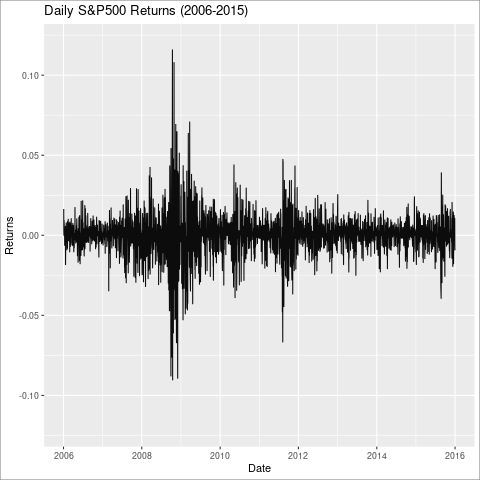
\includegraphics[scale=.45]{plot0615}
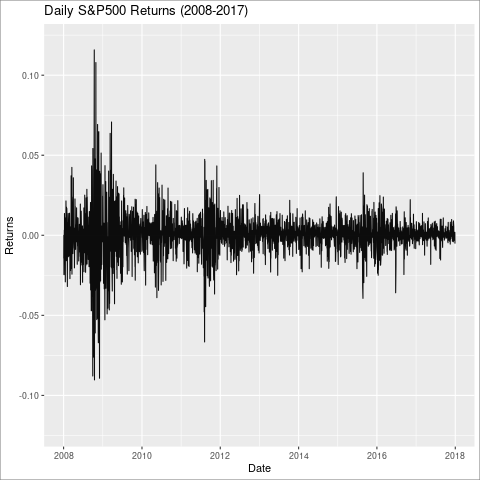
\includegraphics[scale=.45]{plot0817}
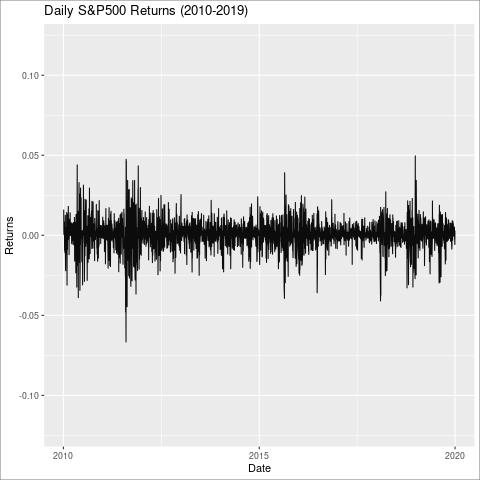
\includegraphics[scale=.45]{plot1019}
\caption{Training Data}
\end{figure}

Returns are normalized: they are calculated by taking the difference between the closing price for a day and the closing price for the previous day, and dividing it by the closing price of the previous day. The code for the data manipulation and setup is available in Appendix A.1. 
\begin{align}
Return_{t} = \frac{ClosingPrice_{t} - ClosingPrice_{t-1}}{ClosingPrice_{t-1}} \nonumber
\end{align}

The models are tested against data from the year immediately following the training period, that is, years 2016, 2018, and 2020. The 2016 test set has 252 observations with minimum -0.0359, maximum 0.0247, mean 0.0003, and standard deviation 0.0082. The 2018 test set has 251 observations with minimum -0.0409, maximum 0.0495, mean -0.0001, and standard deviation 0.0107. The 2020 test set has 253 observations with minimum -0.1198, maximum 0.0938, mean 0.0008, and standard deviation 0.0216. 

\begin{figure}
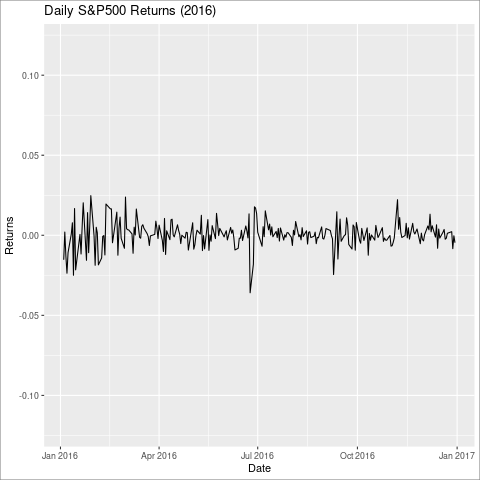
\includegraphics[scale=.5]{plot16}
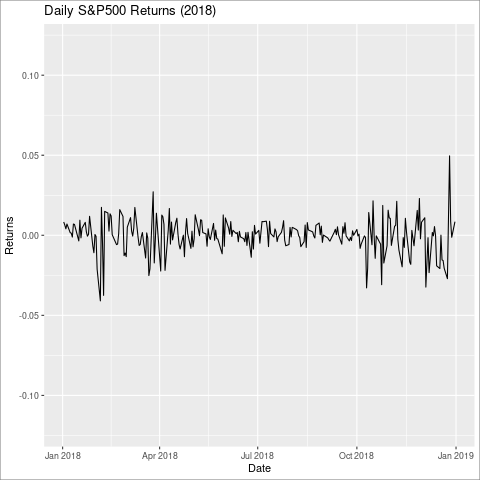
\includegraphics[scale=.5]{plot18}
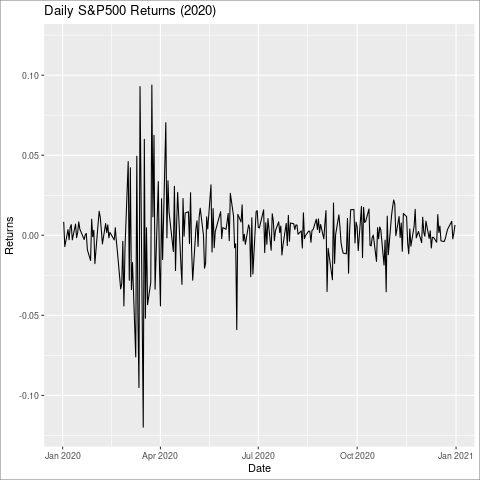
\includegraphics[scale=.5]{plot20}
\caption{Testing Data}
\end{figure}

\subsection{Models}
The two models are specified below. The Stan model codes are available in Appendix A.2. Both contain a log of volatility term, which is simply a transformation of variance.
\begin{align}
\lambda_t & = \ln(\sigma^2_t)
\implies \sigma_t = \exp(\lambda_t/2) 
\end{align}

\subsubsection{GARCH(1,1)}
The Generalized Autoregressive Conditional Heteroskedasticity model used here is specified below. This is a GARCH(1,1) model: it uses the return and volatility from one period prior to compute the volatility for the current period. Let $r_t$ denote the return at time $t$, which depends on $\mu$, the mean return, and $\lambda_t$, the log of volatility (variance) at time $t$. Furthermore, $\alpha_0$, $\alpha_1$, and $\beta_1$ are all positive, and $\alpha_1 + \beta_1 < 1$.  
\begin{align}
r_t &\sim Normal\bigl(\mu, \exp(\lambda_t/2)\bigr) \\
\mu &\sim Cauchy(0, 10) \\
\lambda_1 &\sim Cauchy(0,10) \\
\lambda_t &= \ln\bigl[\alpha_0 + \alpha_1 r_{t-1}^2 + \beta_1 \exp(\lambda_{t-1})\bigr] \\
\alpha_0  &\sim LogNormal(0,1) \\
\alpha_1 &\sim Uniform(0,1) \\
\beta_1 &\sim Uniform(0, 1 - \alpha_1)
\end{align}

The key parameters of the model are $\mu$, $\alpha_0$, $\alpha_1$, and $\beta_1$. These are used to predict $\lambda_t$, which is then used to estimate $r_t$. 

\subsubsection{Stochastic Volatility}
The Stochastic Volatility model is specified below. The return, $r_t$, depends on the mean, $\mu$, and log volatility, $\lambda_t = \ln(\sigma^2_t)$. Persistence of volatility is given by $\phi$, which is between -1 to 1, and the white noise scaling factor is given by $\tau$.

\begin{align}
r_t &\sim Normal\bigl(\mu, \exp({\lambda_t/2})\bigr) \\
\mu &\sim Cauchy(0, 10) \\
\lambda_1 &\sim Normal(\eta, \tau) \\
\lambda_t &\sim Normal\bigl(\eta + \phi(\lambda_{t-1} - \eta), \tau\bigr) \\
\eta &\sim Cauchy(0, 10) \\
\tau &\sim Cauchy(0, 10) \\
\phi &\sim Uniform(-1, 1)
\end{align}

The parameters of the model $\mu$, $\eta$, $\tau$, and $\phi$ are used to find $\lambda_t$, which is then used to estimate $r_t$. A key difference between the two approaches is that GARCH provides a deterministic representation of $\lambda_t$, whereas the Stochastic Volatility model provides, as the name suggests, a stochastic representation of $\lambda_t$.

Both models are coded in the probabilistic programming language Stan, which uses the adaptive variant of Hamiltonian Monte Carlo (HMC) called the No U-Turn Sampler (NUTS) proposed by Hoffman \& Gelman [2014]. Stan is designed to facilitate Bayesian inference for continuous-variable models using Monte Carlo methods [Carpenter et al., 2017].

\subsection{Hamiltonian Monte Carlo | Motivation}
Questions in statistics such as calculating means, medians, variance, and other higher moments involve computing expectations, which necessarily require solving some integration problem. Simple integrals have analytical solutions; but, often we need to integrate over complex distributions, and these integrals do not yield to closed forms. Markov Chain Monte Carlo (MCMC) methods are often used in these instances to derive sampling distibutions, which can then be used to approximate the required integrals.

MCMC algorithms typically use some transition operator satisfying the reversibility condition to move through the space of possible points from the target distribution. The operator specifies the transition probabilities between two points in the distribution. The algorithm is used to take a point $\theta_{previous}$ to the next point $\theta_{current}$, which is then appended to the Markov Chain. The algorithm is repeated multiple times, each time appending a point to the chain. The reversibility condition guarantees that the chain will eventually reach a stationary distribution, and beyond that, the chain, as it grows, will continue to remain within the stationary distribution. This stationary distribution is the target distribution (by design of the transition operator). Thus, as the chain grows longer, the values of the points in the chain begin to approximate the target distribution.

Different MCMC techniques exist for exploring the target distribution. Common MCMC methods include Random Walk Metropolis Sampling (RWMS) and Gibbs Sampling. These algorithms are simple to implement, however, in high dimesional parameter spaces with correlated parameters, RWMS and Gibbs Sampling prove to be inefficient as they make too many poor proposals (proposals that are accepted but too close to the current parameter value, or those that are distant from the current parameter value but from regions with low or no probability mass and hence rejected). In these cases, RWMS and Gibbs Sampling would require the Markov Chains to be inordinately long to sufficiently explore the regions of the target distribution where the probability mass is concentrated, and achieving this length would be computationally prohibitive. If, on the other hand, to make the chain computationally manageable, the algorithm is stopped before sufficient exploration, the expectations derived from the samples would be severely biased.

In high dimensional parameter spaces that are continuous and differentiable (as is the case with the two models specified above), Hamiltonian Monte Carlo (HMC) provides a solution to this exploration issue. The HMC Markov Chains are very efficient as consecutive points in each chain tend to be both far apart in the parameter space and from regions with high probability mass. The presence of high correlation between parameters does not hinder the exploration process of this MCMC algorithm. And while the generation of each new point in the sampling distribution involves more computation than in RWMS or Gibbs Sampling, many fewer points need to be generated to sufficiently cover the target space, leading to overall computational savings [Neal, 2011; Betancourt, 2017].

The general idea for HMC is as follows. We augment the $b$-dimensional parameter space with another set of $b$ auxiliary variables, one for each parameter. In this augmented $2b$-dimensional parameter space, the algorithm traverses from one point to another by following a long trajectory governed by Hamiltonian dynamics. This new point is then projected down to the original $b$-dimensional parameter space. The projected point is located in a region of high probability mass within the original parameter space, and yet is far away from the projection of the point that began the trajectory. This process is repeated and an efficient representative sample in the $b$-dimensional parameter space is derived [Neal, 2011; Betancourt, 2017]. 

\subsection{Hamiltonian Monte Carlo | Method}
For the GARCH model, $\theta = (\mu, \alpha_0, \alpha_1, \beta_1, \lambda_1, \lambda_2, ... , \lambda_T)$ where $T$ is the number of days in the training set for which we have a return value. Here, the dimension of the parameter space is $b = 4 + T$. 

Likewise, for the Stochastic Volatility model, $\theta = (\mu, \eta, \tau, \phi, \lambda_1, \lambda_2, ... , \lambda_T)$ where $T$ is the number of days in the training set for which we have a return value. Again, the dimension of the parameter space is $b = 4 + T$.

Details of the Hamiltonian Monte Carlo algorithm that follow are adaped from Neal [2011] and Betancourt [2017]. The HMC algorithm requires us to provide two functions: the natural logarithm of the joint distribution of the parameters, $\ln\pi(\theta)$, and the gradient of this function in all directions, $\frac{\partial \ln\pi(\theta)}{\partial \theta}$. This gradient (upon some modification) will guide the trajectory of the exploration. The subsequent steps in the HMC algorithm are as follows.

\begin{enumerate}
\item We augment $\theta$ with auxiliary variables $m$. Each parameter in $\theta$ has a corresponding auxiliary variable. Thus, $Dim(\theta) = Dim(m)$, say $b$. The augmented parameter space, $(\theta, m)$ is $2b$-dimensional. It is in this extended space that the algorithm will traverse.
\item Next, we define the Hamiltonian function, $H(\theta, m)$ as the negative of the natural logarithm of the joint density of the parameters and the auxiliary variables, that is, the augmented parameter space.
\begin{align}
H(\theta, m) \coloneqq - \ln \pi(\theta, m)
\end{align}
\item The Hamiltonian function decomposes as follows. 
\begin{align}
H(\theta, m) &= - \ln \pi(\theta, m) \\ \nonumber
&= - \ln [\pi(m | \theta). \pi(\theta)] \\ \nonumber
&= -\ln \pi(m | \theta) - \ln \pi(\theta)
\end{align}
Let $K(m, \theta) \coloneqq -\ln \pi(m | \theta)$ and $V(\theta) \coloneqq - \ln \pi(\theta)$. Note $V(\theta)$ follows from the specification of the target distribution. Any choice for the distribution of $\pi(m|\theta)$ would make the HMC valid. However, for simplicity and efficiency, the standard multivariate normal distribution is often chosen. Stan performs Euclidean HMC, which uses the standard multivariate normal distribution for $\pi(m|\theta)$ as well. 
\item The evolution of $\theta$ and $m$ is governed by the following Hamilton's equations.
\begin{align}
\frac{d\theta}{d\iota} &= \frac{\partial H(\theta, m)}{\partial m} \\ \nonumber
&= \frac{\partial[K(m, \theta) + V(\theta)]}{\partial m} \\ \nonumber
&= \frac{\partial K(m, \theta)}{\partial m}
\end{align}
\begin{align}
\frac{d m}{d \iota} &= - \frac{\partial H(\theta, m)}{\partial \theta} \\ \nonumber
&= - \frac{\partial[K(m, \theta) + V(\theta)]}{\partial \theta} \\ \nonumber
&= - \frac{\partial K(m, \theta)}{\partial \theta} - \frac{\partial V(\theta)}{\partial \theta}
\end{align}
Here $\iota$ is an imaginary time-step. $\frac{\partial V(\theta)}{\partial \theta}$ follows from the gradients provided to the HMC function. The differential equations in (31) and (32) together define a vector field, the contours of which align with the high mass regions in the parameter space. 
\end{enumerate}

Stan uses autodifferentiation [Carpenter et al., 2015] to construct the derivatives above. In addition to the two functions, the implementation of HMC in Stan requires two other quantities: stepsize and number of leapfrog steps. The stepsize governs the length of the imaginary time-step mentioned in step (4). The number of leapfrog steps governs how many imaginary time-steps forward the parameter is propagated in order to arrive at the new proposed parameter. 

In practice, depending on the terrain of the joint posterior, for certain values of stepsize and number of leapfrog steps, it is possible for the algorithm to generate trajectories that loop back to or near the starting point, and hence be inefficient. The right selection of stepsize and number of leapfrog steps is important for efficient exploration.

Stan uses the adaptive variant of HMC called the No U-Turn Sampler (NUTS) to avoid these inefficiencies. The NUTS algorithm uses iterations in the warmup period to automatically test various stepsizes and number of leapfrog steps and optimize these two quantitites [Carpenter et al., 2017].  

\subsection{Parameter Estimation}
For the GARCH model, 50,000 iterations are run on 4 chains each. 50\% of the iterations are used for warmup, resulting in a posterior sample of 100,000 points in total.  

For the Stochastic Volatility model, 1,000,000 iterations are run on 4 chains for 100,000 iterations each. Half of the iterations are used up in the warmup phase, and one out of 20 successive points is selected resulting again in 100,000 points from the posterior distribution. More iterations and thinning are used in this model to compensate for slower convergence and higher autocorrelation in parameters $\phi$ and $\tau$. 

The code used for fitting the models is available in Appendix A.3.

\subsection{Parameter Updates}
Updating parameters involves the Sequential Monte Carlo step of assigning weights to each of the 100,000 points from the posterior distribution and then resampling (with replacement) as many points according to these weights whenever the Effective Sample Size (ESS) drops under an acceptable threshold (set, here, at 0.9). Details of this method are listed in Capp\'{e} [2007].

The Effective Sample Size (ESS) quantifies the amount of independent information or effective data points in a sample. In Markov Chain Monte Carlo procedures (including Hamiltonian Monte Carlo, the procedure used in this paper), the goal is to generate a sequence of correlated samples from a target distribution to estimate various properties of interest. However, due to the inherent correlation between successive samples in the chains generated, the effective amount of independent information is typically lower than the actual sample size. The ESS is calculated as follows. 
\begin{align}
ESS = \frac{\text{N}}{1 + 2\sum_{t=1}^{\infty}\rho_t}
\end{align}
Where $N$ is the number of iterations, and $\rho_t$ is the autocorrelation corresponding to a lag of $t$ time units.

The weights are determined using the Gaussian density function on the predicted return at each point. That is, given the mean and standard deviation (a tansformation of lambda) corresponding to a point, the point will have a higher weight if the Gaussian density for its predicted return is higher, and vice versa. The weights are normalized by the sum of all the weights. Whenever, over the course of iterated propagation (described in section 3.8 below), the ESS falls below the specified threshold, the cloud of 100,000 points are resampled with replacement according to these normalized weights. 

Appendix A.4 provides the code for assigning weights and resampling.

\subsection{Prediction and Propagation}
Using the parameters found above, each point at time $t$ is used to predict the point at time $t+1$. Lambda at time $t+1$ is estimated first using the parameters at time $t$, and then $\lambda_{t+1}$ (along with other parameters) is used to generate return at time $t+1$. 

``Propagation" refers to moving the cloud of 100,000 points one step forward. Before each propagation, we check the effective sample size and resample if necessary. The  propagation is done for each month, each quarter, and for the whole year, for the years 2016, 2018, and 2020. 

Appendix A.4 contains the code for prediction and propagation.

\subsection{Performance Comparison}
After the predicted returns are calculated by both models for the three different time-frames, the results are tested against the returns data for 2016, 2018, and 2020 using the sum of squared errors. The empirical distributions of predictions are used to compute the fraction of the observed returns data that fall within the 2.5 percentile and the 97.5 percentile of the predicted returns.  

Appendix A.5 provides the performance comparison code. 

\newpage
\section{Results}

\subsection{GARCH Parameter Estimates}
Figures 1-3 below contain the histograms of the 100,000 point posterior samples generated from the GARCH model.

\subsubsection{2006-15}
\begin{figure}
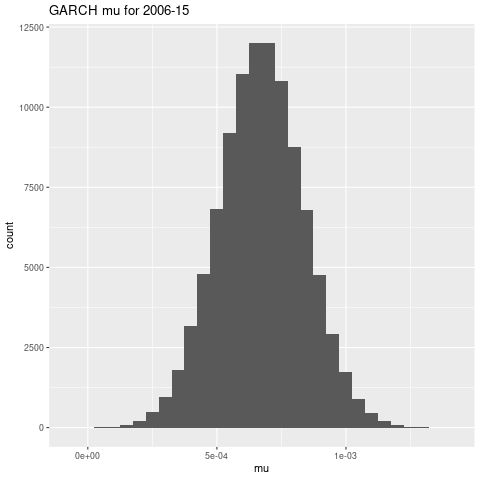
\includegraphics[scale = .4]{gmu0615}
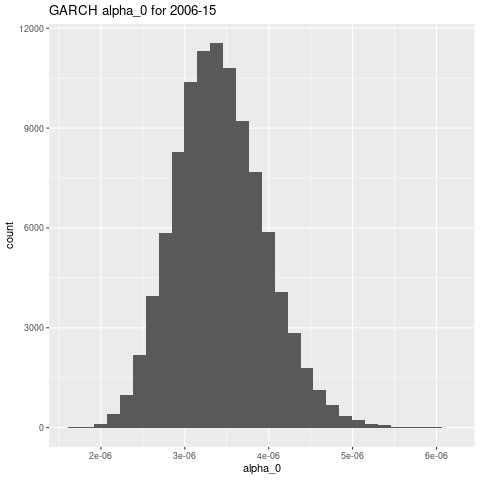
\includegraphics[scale = .4]{ga00615}
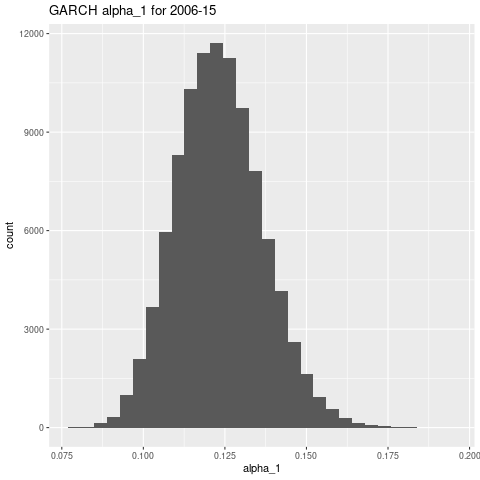
\includegraphics[scale = .4]{ga10615}
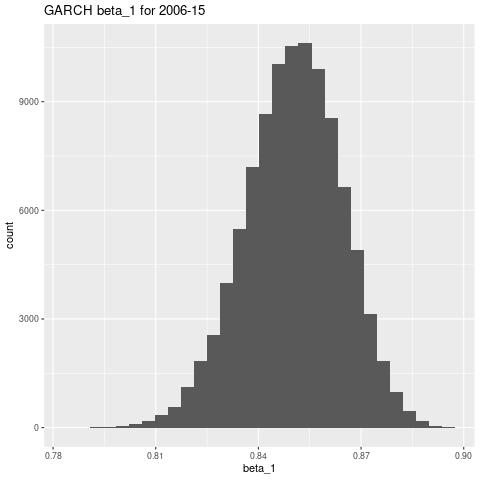
\includegraphics[scale = .4]{gb10615}
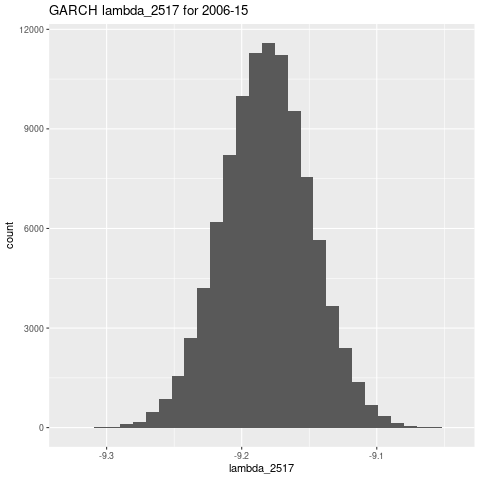
\includegraphics[scale = .4]{glT0615}
\caption{GARCH posterior samples for 2006-15 training data.}
\end{figure}

The mean estimates for the parameters are as follows.
\begin{align*}
\mu &= 0.0006 \\
\alpha_0 &= 0.0000 \\
\alpha_1 &= 0.1235 \\
\beta_1 &= 0.8502
\end{align*}

The lambda corresponding to the last time period in the training set has a mean of $-9.1817$.

\subsubsection{2008-17}
\begin{figure}
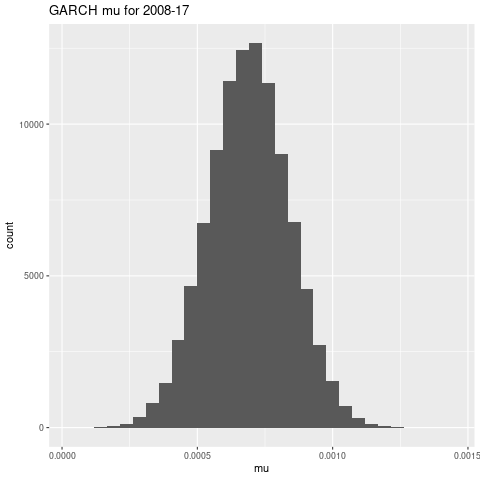
\includegraphics[scale = .4]{gmu0817}
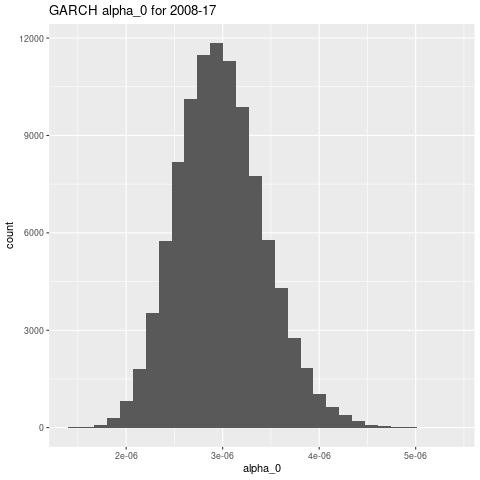
\includegraphics[scale = .4]{ga00817}
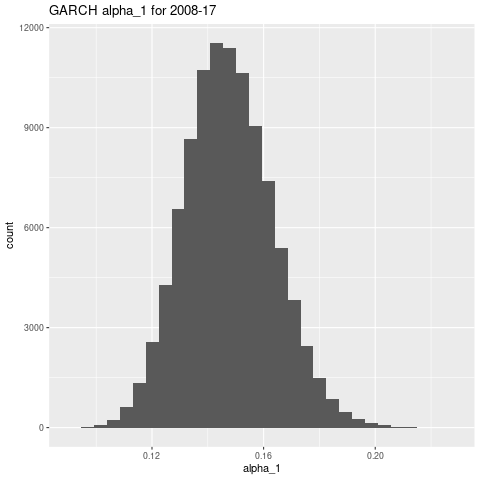
\includegraphics[scale = .4]{ga10817}
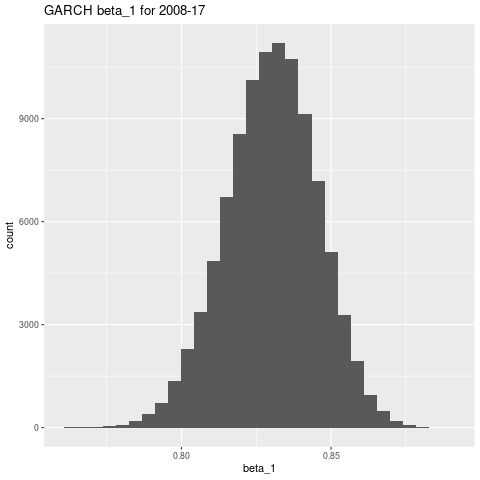
\includegraphics[scale = .4]{gb10817}
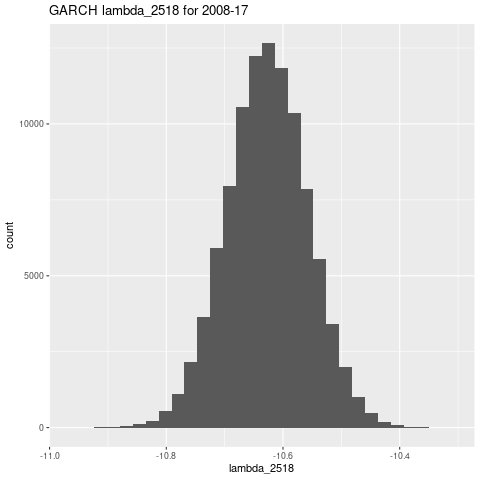
\includegraphics[scale = .4]{glT0817}
\caption{GARCH posterior samples for 2008-17 training data.}
\end{figure}

The mean estimates for the parameters are as follows.
\begin{align*}
\mu &= 0.0006 \\ 
\alpha_0 &= 0.0000 \\ 
\alpha_1 &= 0.1475 \\ 
\beta_1 &= 0.8300 
\end{align*}

The lambda corresponding to the last time period in the training set has a mean of $-10.6268$.

\subsubsection{2010-19}
\begin{figure}
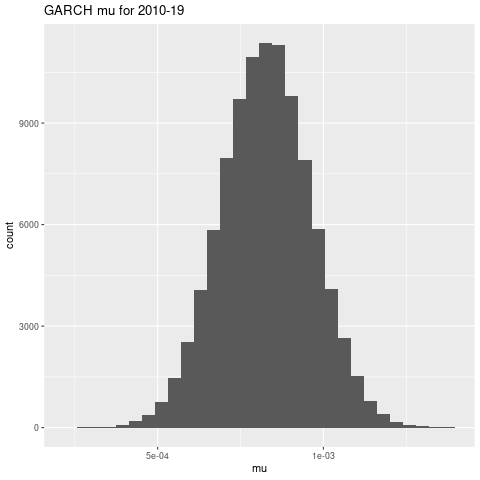
\includegraphics[scale = .4]{gmu1019}
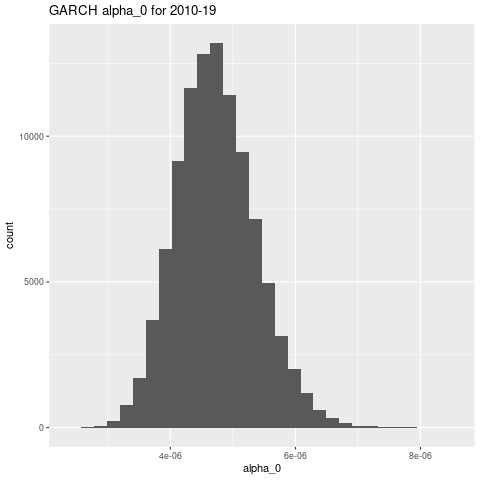
\includegraphics[scale = .4]{ga01019}
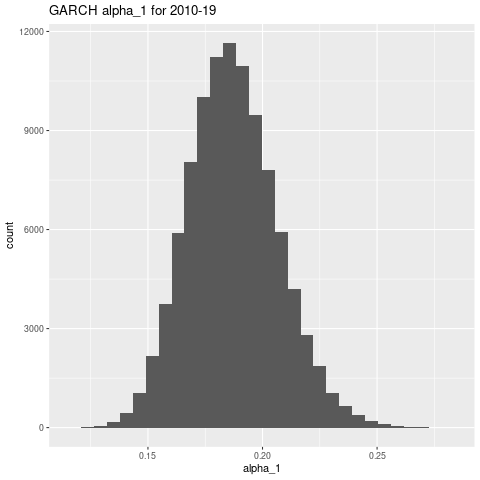
\includegraphics[scale = .4]{ga11019}
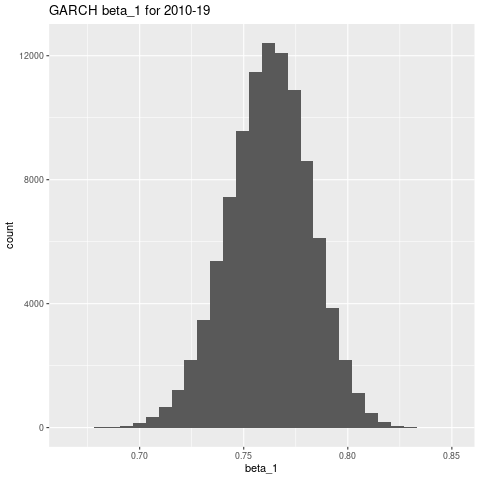
\includegraphics[scale = .4]{gb11019}
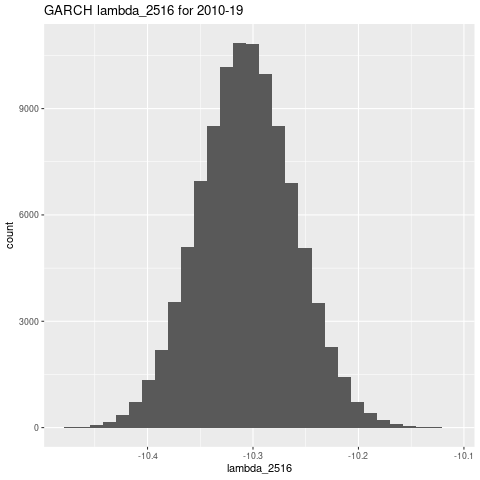
\includegraphics[scale = .4]{glT1019}
\caption{GARCH posterior samples for 2010-19 training data.}
\end{figure}

The mean estimates for the parameters are as follows.
\begin{align*}
\mu &= 0.0008 \\ 
\alpha_0 &= 0.0000 \\ 
\alpha_1 &= 0.1871 \\ 
\beta_1 &= 0.7621 
\end{align*}

The lambda corresponding to the last time period in the training set has a mean of $-10.3061$.

\subsection{Stochastic Volatility Parameter Estimates}
The histograms of the 100,000 point posterior samples generated from the Stochastic Volatility model are as follows.

\subsubsection{2006-15}
\begin{figure}
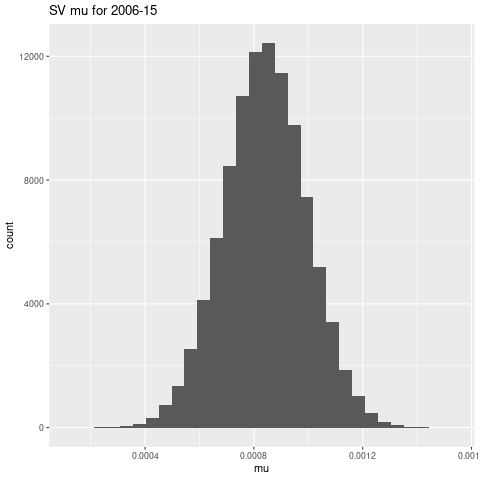
\includegraphics[scale = .4]{svmu0615}
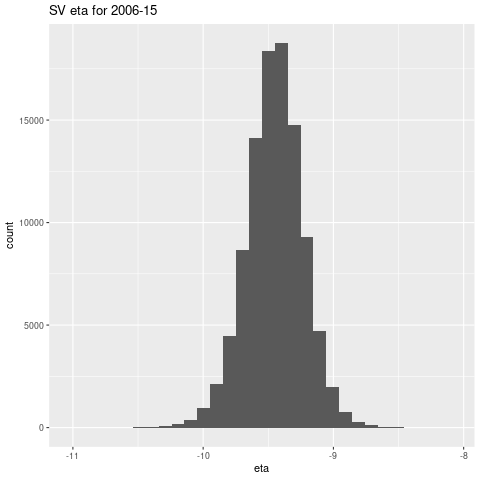
\includegraphics[scale = .4]{sve0615}
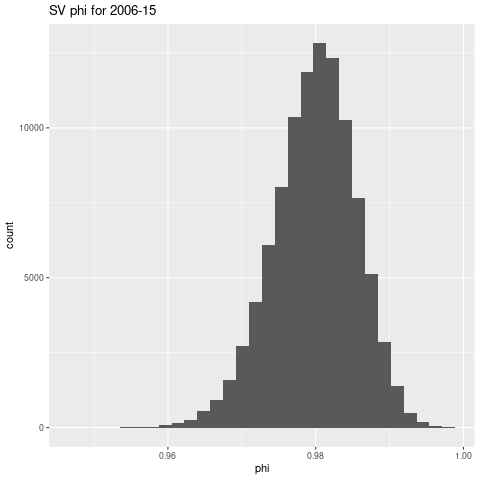
\includegraphics[scale = .4]{svp0615}
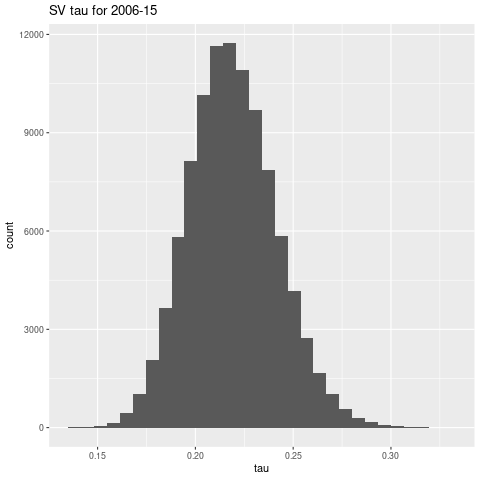
\includegraphics[scale = .4]{svt0615}
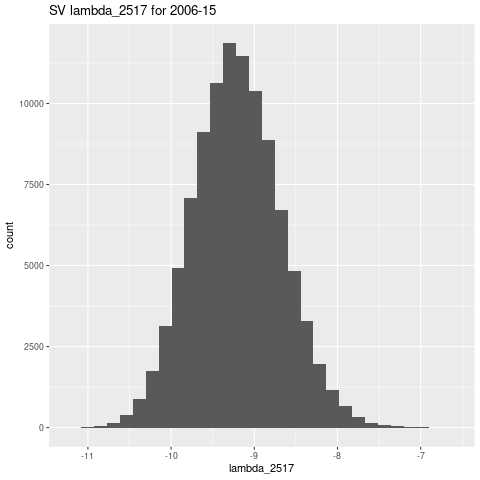
\includegraphics[scale = .4]{svlT0615}
\caption{Stochastic Volatility posterior samples for 2006-15 training data.}
\end{figure}

The Stochastic Volatility parameter estimates using mean values are below in figures 4-6.
\begin{align*}
\mu &= 0.0008 \\
\eta &= -9.4503 \\
\phi &= 0.9798 \\
\tau &= 0.2190 
\end{align*}

The lambda corresponding to the last time period in the training set has a mean of $-9.2065$.

\subsubsection{2008-17}
\begin{figure}
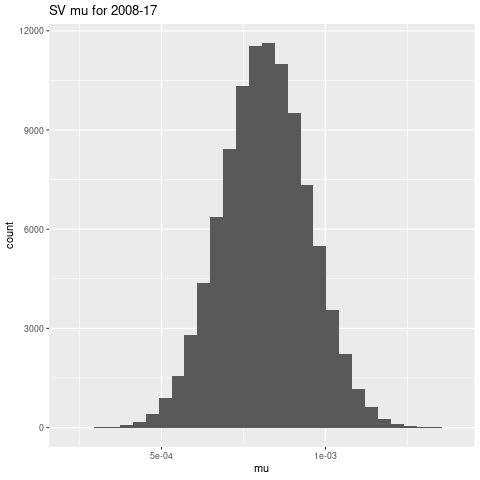
\includegraphics[scale = .4]{svmu0817}
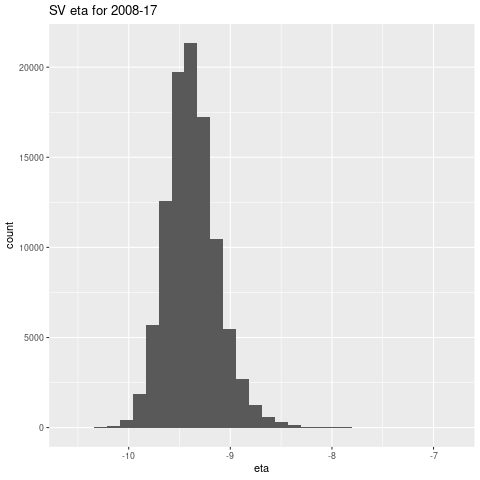
\includegraphics[scale = .4]{sve0817}
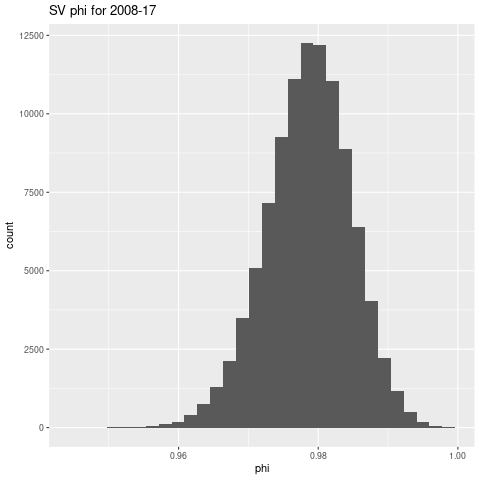
\includegraphics[scale = .4]{svp0817}
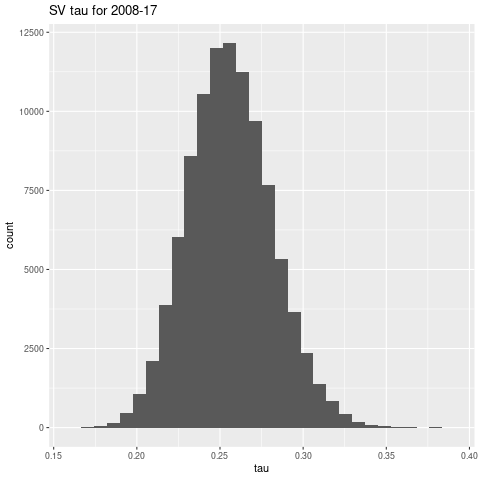
\includegraphics[scale = .4]{svt0817}
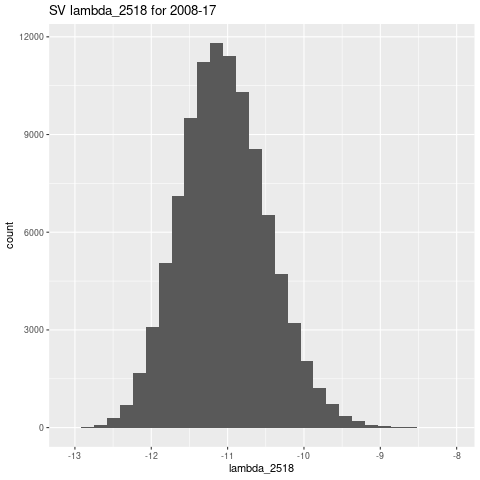
\includegraphics[scale = .4]{svlT0817}
\caption{Stochastic Volatility posterior samples for 2008-17 training data.}
\end{figure}

The Stochastic Volatility parameter estimates using mean values are below in figures 4-6.
\begin{align*}
\mu &= 0.0008 \\
\eta &= -9.3779 \\
\phi &= 0.9785 \\
\tau &= 0.2560
\end{align*}

The lambda corresponding to the last time period in the training set has a mean of $-11.0425$.

\subsubsection{2010-19}
\begin{figure}
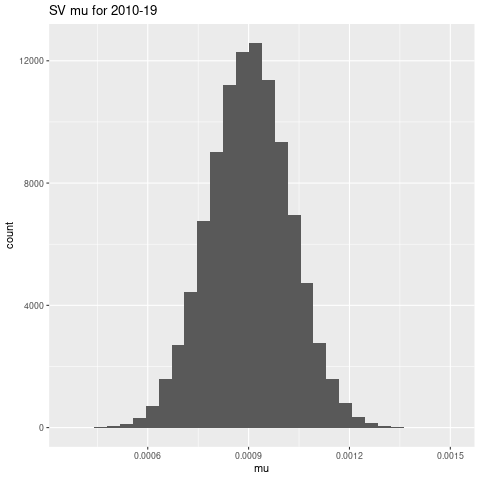
\includegraphics[scale = .4]{svmu1019}
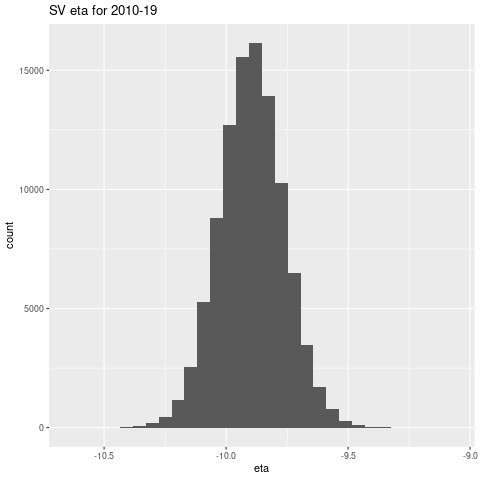
\includegraphics[scale = .4]{sve1019}
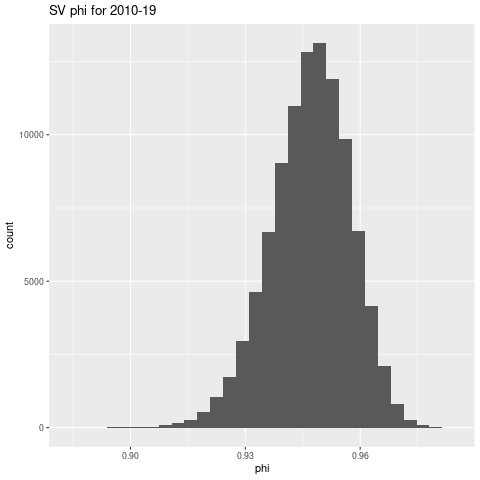
\includegraphics[scale = .4]{svp1019}
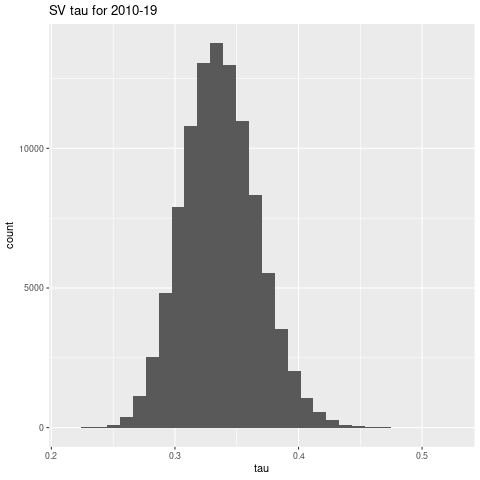
\includegraphics[scale = .4]{svt1019}
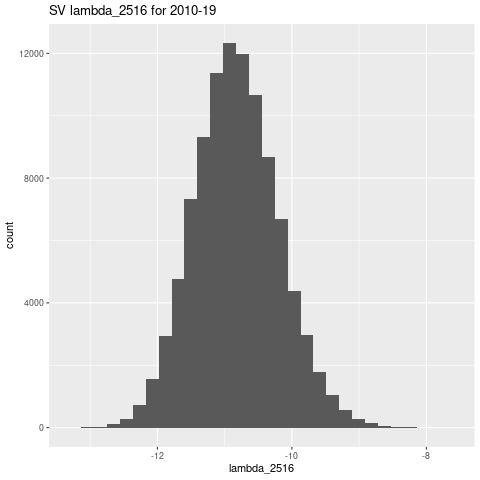
\includegraphics[scale = .4]{svlT1019}
\caption{Stochastic Volatility posterior samples for 2010-19 training data.}
\end{figure}

The Stochastic Volatility parameter estimates using mean values are below in figures 4-6.
\begin{align*}
\mu &= 0.0009 \\
\eta &= -9.8949 \\
\phi &= 0.9469 \\
\tau &= 0.3366
\end{align*}

The lambda corresponding to the last time period in the training set has a mean of $-10.8228$.

\subsection{Comparing Sum of Squared Errors of Estimated Returns}
The parameter estimates obtained above for the GARCH and the Stochastic Volatility models are used to (a) estimate the hidden variable, lambda, and (b) predict the return, for the next time step. This is done for the entire cloud of 100,000 points. Then, the parameters are updated using the parameter update step described above. Next, the estimation of lambda and prediction of return for the subsequent time step are done. The execution details are in Appendix A.4.

The code in Appendix A.4 generates predictions for the years 2016 (a low volatility year), 2018 (medium volatility year) and 2020 (a high volatility year). These predictions are compared against the test data from 2016, 2018 and 2020 using sum of squared errors. Appendix A.5 contains the corresponding comparison code. Tables 1-3 present the SSE for the two models for the three years along with an indicator for which model has the lower SSE.

\begin{table}[!ht]
    \centering
    \begin{tabular}{|l|l|l|l|}
    \hline
        ~ & \textbf{GARCH} & \textbf{SV} & \textbf{Result} \\ \hline
        \textbf{Month 1 }& 0.0047 & 0.0047 & Equal \\ \hline
        \textbf{Month 2} & 0.0027 & 0.0027 & Equal \\ \hline
        \textbf{Month 3} & 0.0006 & 0.0006 & Equal \\ \hline
        \textbf{Month 4} & 0.0009 & 0.0009 & Equal \\ \hline
       \textbf{Month 5} & 0.0008 & 0.0008 & Equal \\ \hline
       \textbf{Month 6} & 0.0028 & 0.0028 & Equal \\ \hline
        \textbf{Month 7} & 0.0004 & 0.0004 & Equal \\ \hline
        \textbf{Month 8} & 0.0002 & 0.0002 & Equal \\ \hline
        \textbf{Month 9} & 0.0016 & 0.0016 & Equal \\ \hline
        \textbf{Month 10} & 0.0003 & 0.0003 & Equal \\ \hline
        \textbf{Month 11} & 0.0009 & 0.0009 & Equal \\ \hline
        \textbf{Month 12} & 0.0005 & 0.0005 & Equal \\ \hline
        \textbf{Quarter 1} & 0.0082 & 0.0082 & Equal \\ \hline
        \textbf{Quarter 2} & 0.0046 & 0.0046 & Equal \\ \hline
        \textbf{Quarter 3} & 0.0024 & 0.0024 & Equal \\ \hline
        \textbf{Quarter 4} & 0.0018 & 0.0018 & Equal \\ \hline
        \textbf{Full Year} & 0.0171 & 0.0171 & Equal \\ \hline
    \end{tabular}
\caption{Sum of Squared Errors for 2016}
\end{table}

\begin{table}[!ht]
    \centering
    \begin{tabular}{|l|l|l|l|}
    \hline
        ~ & \textbf{GARCH} & \textbf{SV} & \textbf{Result} \\ \hline
        \textbf{Month 1} & 0.0007 & 0.0007 & Equal \\ \hline
        \textbf{Month 2} & 0.0056 & 0.0056 & Equal \\ \hline
        \textbf{Month 3} & 0.0037 & 0.0037 & Equal \\ \hline
        \textbf{Month 4} & 0.0017 & 0.0017 & Equal \\ \hline
        \textbf{Month 5} & 0.0009 & 0.0009 & Equal \\ \hline
        \textbf{Month 6} & 0.0005 & 0.0005 & Equal \\ \hline
        \textbf{Month 7} & 0.0006 & 0.0006 & Equal \\ \hline
        \textbf{Month 8} & 0.0004 & 0.0004 & Equal \\ \hline
        \textbf{Month 9} & 0.0002 & 0.0002 & Equal \\ \hline
        \textbf{Month 10} & 0.0045 & 0.0045 & Equal \\ \hline
        \textbf{Month 11} & 0.0028 & 0.0028 & Equal \\ \hline
        \textbf{Month 12} & 0.0069 & 0.0069 & Equal \\ \hline
        \textbf{Quarter 1} & 0.0100 & 0.0100 & Equal \\ \hline
        \textbf{Quarter 2} & 0.0032 & 0.0032 & Equal \\ \hline
        \textbf{Quarter 3} & 0.0012 & 0.0012 & Equal \\ \hline
        \textbf{Quarter 4} & 0.0144 & 0.0144 & Equal \\ \hline
        \textbf{Full Year} & 0.0290 & 0.0290 & Equal \\ \hline
    \end{tabular}
\caption{Sum of Squared Errors for 2018}
\end{table}

\begin{table}[!ht]
    \centering
    \begin{tabular}{|l|l|l|l|}
    \hline
        ~ & \textbf{GARCH} & \textbf{SV} & \textbf{Result} \\ \hline
        \textbf{Month 1} & 0.0011 & 0.0011 & Equal \\ \hline
        \textbf{Month 2} & 0.0078 & 0.0078 & Equal \\ \hline
        \textbf{Month 3} & 0.0724 & 0.0724 & Equal \\ \hline
        \textbf{Month 4} & 0.0129 & 0.0129 & Equal \\ \hline
        \textbf{Month 5} & 0.0032 & 0.0032 & Equal \\ \hline
        \textbf{Month 6} & 0.0071 & 0.0071 & Equal \\ \hline
        \textbf{Month 7} & 0.0015 & 0.0015 & Equal \\ \hline
        \textbf{Month 8} & 0.0006 & 0.0006 & Equal \\ \hline
        \textbf{Month 9} & 0.0049 & 0.0049 & Equal \\ \hline
        \textbf{Month 10} & 0.0035 & 0.0035 & Equal \\ \hline
        \textbf{Month 11} & 0.0025 & 0.0025 & Equal \\ \hline
        \textbf{Month 12} & 0.0006 & 0.0005 & SV is lower \\ \hline
        \textbf{Quarter 1} & 0.0814 & 0.0813 & SV is lower \\ \hline
        \textbf{Quarter 2} & 0.0233 & 0.0233 & Equal \\ \hline
        \textbf{Quarter 3} & 0.0071 & 0.0071 & Equal \\ \hline
        \textbf{Quarter 4} & 0.0066 & 0.0066 & Equal \\ \hline
        \textbf{Full Year} & 0.1185 & 0.1185 & Equal \\ \hline
    \end{tabular}
\caption{Sum of Squared Errors for 2020}
\end{table}

\newpage
\subsection{Comparing Capture in 95 Percent Band}
The empirical distributions of the predicted returns for 2016, 2018, and 2020 are used to find the predictions at the 2.5 percentile and the 97.5 percentile for both models in each day of the three years. For the GARCH model, the 95 percent prediction band captured 238 out of 252 observations in 2016; 243 out of 251 observations in 2018; and 206 out of 253 observations in 2020. 
For the Stochastic Volatility model, the 95 percent prediction band captured 237 out of 252 observations in 2016; 242 out of 251 observations in 2018; and 203 out of 253 observations in 2020. The corresponding code is in Appendix A.5.

\newpage
\section{Discussion}
In terms of SSE, both models perform nearly identically across all time-frames and in all three time periods. Small differences in the sum of squared errors arise, usually, in the ten-thousandths place or later. These small differences can be attributed to the monte carlo errors associated with the computations. 

Out of the twelve month long time-frames assessed for 2016, the GARCH and the Stochastic Volatility results are indistinguishable in every month. These SSEs range from a low of 0.0002 to a high of 0.0047 for both estimates. The highs and the lows occur on the same months for both the models.

Out of the twelve month long time-frames assessed for 2018, the GARCH and the Stochastic Volatility results are indistinguishable in every month. These SSEs range from a low of 0.0002 to a high of 0.0069 for the both estimates. The highs and the lows occur on the same months for both the models.

Out of the twelve month long time-frames assessed for 2020, the GARCH results are indistinguishable from the Stochastic Volatility results on 11 occasions. The only small noticeable difference occur in month 12, for which the Stochastic Volatility estimate shows a lower sum. These SSEs range from a low of 0.0006 to a high of 0.0724 for the GARCH estimates, while for the Stochastic Volatility estimates, they range from a low of 0.0005 to a high of 0.0724. The highs and the lows occur on the same months for both the models.

Out of the four quarters assessed for 2016, GARCH and Stochastic Volatility perform equally well in every quarter. These SSEs range from a low of 0.0018 to a high of 0.0082 for both estimates. The highs and the lows for both models occur in the same quarters.  

Out of the four quarters assessed for 2018, GARCH and Stochastic Volatility perform equally well in every quarter. These SSEs range from a low of 0.0012 to a high of 0.0144 for both estimates. The highs and the lows for both models occur in the same quarters.

Out of the four quarters assessed for 2020, GARCH and Stochastic Volatility are indistinguishable in every quarter except the first. In quarter 1, the sum for Stochastic Volatility is slightly lower. The SSEs range from a low of 0.0066 to a high of 0.0814 for the GARCH estimates, while for the Stochastic Volatility estimates, they range from a low of 0.0066 to a high of 0.0813. The highs and the lows for both models occur in the same quarters.  

For every full year assessed, the GARCH and the Stochastic Volatility models deliver identical results. For 2016, the full-year SSE is 0.0171. For 2018, the full-year SSE is 0.0290. For 2020, despite small differences in monthly or quarterly results, the full-year SSE is 0.1185 for both models. 

In general, we notice that the models have the least SSE in the low volatility year (2016) and the highest SSE in the high volatility year (2020).
The differences in the predictive performance between the two models are not practically significant. When one model has low SSE, the other model has low SSE too, and when one has high SSE, the other shows similar effect. The small differences that arise can be attributed to the randomness involved in the prediction process. 

The 95 percent prediction bands perform similarly for both models as well. In 2016, the prediction bands for the GARCH model capture 238 out of 252 observations (94.44\% accuracy) while those for the Stochastic Volatility model capture 237 out of 252 observations (94.04\% accuracy). In 2018, they capture 243 out of 251 observations (96.81\% accuracy) for GARCH, and 242 out of 251 observations for Stochastic Volatility (96.41\% accuracy). Finally, in 2020, they capture 206 out of 253 observations for GARCH (81.42\% accuracy), and 203 out of 253 observations for Stochastic Volatility (80.23\% accuracy). While the GARCH model is slightly more predictive in each year above, they differ by only one day. Also, in the high-volatility year of 2020, the predictive accuracy of both models reduce significantly. Hence, in practical terms, both models are indistinguishable. 


\newpage
\section{Further Studies}
This paper uses various ten-year daily returns of the S\&P-500 Index from 2006 to 2020 to make parameter estimates and predictions. Sections 4.1 and 4.2 provide the distributions of the parameter estimates for the GARCH and Stochastic Volatility models, but immediately reduce the results to point estimates for subsequent analysis. The distributions themselves remain under-explored. Further studies might take into account the full distributions of these parameters for generating predictions. 

The compression of distribution-based outputs to single points can be seen again in section 4.3 where the computation of SSE necessitates the use of the mean of the daily predicted return values. This has the effect of producing results nearly identical to those obtained simply by computing SSEs with the fixed $\mu$s generated by each HMC simulation but at significantly higher computational costs. While section 4.4 makes use of the empirical distribution of the predictions to ascertain whether the observations fall within the 2.5 percentile and the 97.5 percentile of predicted returns for each day of the test years, the distribution properties of the predictions remain under-utilized. 

Further study could include an analysis of distribution-based properties such as the width of the prediction bands and the thickness of the tails. For instance, the outputs of the Stochastic Volatility models generally result in greater kurtosis in all three test years. (In 2016, the skewness of the distribution of kurtosis of the daily predicted returns for the GARCH model is 0.1964 as opposed to 1.0573 for the Stochastic Volatility model. This implies that the kurtosis of daily returns is more right-skewed for the Stochastic Volatility model, further implying that the distribution of predicted returns from the Stochastic Volatility model is thicker-tailed. This result holds for 2018 with the skewness of the kurtosis at 1.0021 for GARCH and 4.8058 for Stochastic Volatility; and for 2020 with the skewness of kurtosis at 1.9687 and 4.4532 for GARCH and Stochastic Volatility respectively. Appendix A.5 contains the corresponding code to generate these results.) An exploration of  the process resulting in these differences and their implications might be of interest, especially when the analysis is done from a risk-management/ruin-avoidance framework (as in Taleb [2020]) rather than a prediction-oriented framework.

Probabilistic forecasting is another approach that may be taken to make claims about the returns predictions. In this case, probabilistic forecasting would generate various ranges of returns and the associated probabilities for observing returns in those ranges. Gneiting \& Katzfuss [2014] describes the method of probabilistic forecasting in further details.

Certain parameters of the models, namely, $\mu$ and $\lambda_1$ for GARCH, and $\mu$, $\eta$, and $\tau$ for Stochastic Volatility begin with noninformative $Cauchy(0,10)$ priors. While this lack of previous information allows for a derivation of the distributions solely based on the training data, the convergence can be vastly sped up by the use of informative priors. The posterior sampling distributions generated in this paper may be used to generate priors in future studies.

Moreover, the methodology used in this paper may also be used on assets other than the S\&P-500 Index. It would be interesting to see how different the results are and whether the prediction accuracy holds for the other assets.

Finally, an aspect of modeling this paper does not cover is computation time. In this study, the parameter estimation for Stochastic Volatility took several times as long as the parameter estimation for GARCH, and yet resulted in similar outputs. Further studies could involve more optimization of the code, closer monitoring of the estimation and prediction times, and use of other software.   

\newpage

\appendix
\section{Codes}

\subsection{Data Preparation and Exploration}
\begin{verbatim}

library(here)
library(tidyverse)
library(vroom) 
library(lubridate)
library(ggplot2)
library(ggthemes)

data = vroom(here("SPX_from_2000_to_2022.csv"))

data = data %>%
  mutate(Date = mdy(Date)) %>%
  arrange(Date) %>%
  mutate(Returns = (Close - lag(Close))/lag(Close)) %>%
  select(c(Date, Returns)) 

data0615 = data %>% filter(Date > "2005-12-31" & Date < "2016-01-01")
data16 = data %>% filter(Date > "2015-12-31" & Date < "2017-01-01")

data0817 = data %>% filter(Date > "2007-12-31" & Date < "2018-01-01")
data18 = data %>% filter(Date > "2017-12-31" & Date < "2019-01-01")

data1019 = data %>% filter(Date > "2009-12-31" & Date < "2020-01-01")
data20 = data %>% filter(Date > "2019-12-31" & Date < "2021-01-01")


png("plot0615.png")
ggplot(data0615, aes(x=Date, y=Returns)) +
  geom_point(alpha=0.25, color = "black") +
  scale_x_date() +
  ylim(-0.12, 0.12) +
  theme(plot.background = element_rect(colour = "grey50")) +
  ggtitle("Daily S&P500 Returns (2006-2015)")
dev.off

png("plot16.png")
ggplot(data16, aes(x=Date, y=Returns)) +
  geom_line(color = "black") +
  scale_x_date() +
  ylim(-0.12, 0.12) +
  theme(plot.background = element_rect(colour = "grey50")) +
  ggtitle("Daily S&P500 Returns (2016)")
dev.off

#repeat for other years

\end{verbatim}

\subsection{Stan Models}
\begin{verbatim}

# install.packages("rstan", 
# repos = "https://cloud.r-project.org", dependencies=TRUE)
library(rstan)

# Stan Models

# GARCH Model:
model_G <- "data {
  int<lower=0> T;
  real r[T];
}
parameters {
  real mu;
  real<lower=0> alpha0;
  real<lower=0, upper=1> alpha1;
  real<lower=0, upper=(1-alpha1)> beta1;
  real lambda1;
}
transformed parameters {
  real lambda[T];
  lambda[1] = lambda1;
  for (t in 2:T) {
    lambda[t] = log(alpha0
                     + alpha1 * pow((r[t - 1] - mu), 2)
                     + beta1 * exp(lambda[t - 1]));
  }
}
model {
  for (t in 1:T) {
    r[t] ~ normal(mu, exp(lambda[t]/2));
  }
  lambda1 ~ cauchy(0,10); 
  alpha0 ~ lognormal(0,1);
  alpha1 ~ uniform(0,1);
  beta1 ~ uniform(0, 1 - alpha1);
  mu ~ cauchy(0, 10);
}"

# Stochastic Volatility Model:
model_SV <- "data {
  int<lower=0> T;   
  real r[T];      
}
parameters {
  real mu;                     
  real eta;
  real<lower=-1, upper=1> phi; 
  real<lower=0> tau;         
  real lambda[T];                
}
model {
  phi ~ cauchy(0, 10);
  tau ~ cauchy(0, 10);
  mu ~ cauchy(0, 10);
  eta ~ cauchy(0, 10);
  lambda[1] ~ normal(eta, tau);
  for (t in 2:T) {
    lambda[t] ~ normal(eta + phi * (lambda[t - 1] -  eta), tau);
  }
  for (t in 1:T) {
    r[t] ~ normal(mu, exp(lambda[t] / 2));
  }
}
"

\end{verbatim}

\subsection{Fitting}
\begin{verbatim}
set.seed(2023)

#libraries
# install.packages("rstan", repos = "https://cloud.r-project.org", 
# dependencies=TRUE)
library(rstan)

data = data0615 # or data0817,1019 as appropriate
len = nrow(data)

# Model Fitting
# The following will generate 100,000 points each.

# GARCH
st_G = Sys.time()
fit_G <- stan(model_code = model_G, data = list(T = len, r = data$Returns), 
iter = 50000, chains = 4, cores = 4)
ed_G = Sys.time()
tt_G = ed_G - st_G

# Stochastic Volatility
st_SV = Sys.time()
fit_SV <- stan(model_code = model_SV, data = list(T = len, r = data$Returns), 
iter = 1000000, chains = 4, cores = 4, thin = 20)
ed_SV = Sys.time()
tt_SV = ed_SV - st_SV

# Saving results (Rename accordingly with 0615, 0817, or 1019)
saveRDS(fit_G, file='fit_G0615.rds')
saveRDS(fit_SV, file='fit_SV0615.rds') 

# Extracting Parameters
parameters_G = extract(fit_G)   # contains mu, alpha0, alpha1, beta1, lambdas
parameters_SV = extract(fit_SV) # contains mu, eta, tau, phi, lambdas

\end{verbatim}

\subsection{Prediction}
\begin{verbatim}

set.seed(2023)

#libraries
library(here)
library(tidyverse)
library(lubridate)
library(ggplot2)
library(ggthemes)
# install.packages("rstan", repos = "https://cloud.r-project.org", 
# dependencies=TRUE)
library(rstan)


# Select appropriate dataset
data = data18

# Read appropriate fit file, 0615, 0817, or 1019
fit_G = readRDS(file = "fit_G0817.rds")
fit_SV = readRDS(file = "fit_SV0817.rds")

# Parameter extraction
parameters_G = extract(fit_G)   # contains mu, alpha0, alpha1, beta1, lambdas
parameters_SV = extract(fit_SV) # contains mu, eta, phi, tau, lambdas



# Creating initial dataframe

df_G = data.frame("mu" = parameters_G$mu, "alpha0" = parameters_G$alpha0,
"alpha1" = parameters_G$alpha1,"beta1"=parameters_G$beta1, 
"lambda_t" = parameters_G$lambda[,nrow(data)])

df_SV = data.frame("mu" = parameters_SV$mu, "eta" = parameters_SV$eta,
"phi" = parameters_SV$phi, "tau"= parameters_SV$tau, 
"lambda_t" = parameters_SV$lambda[,nrow(data)])

pred_returns_G = mapply(function(mean, sd) {rnorm(1, mean, sd)}, df_G$mu,
exp(df_G$lambda_t/2))

pred_returns_SV = mapply(function(mean, sd) {rnorm(1, mean, sd)},
df_SV$mu, exp(df_SV$lambda_t/2))
### this has the same effect as
###for (i in 1:nrow(df_G)) {
###  pred_returns[i] = rnorm(1, mean=df_G$mu[i], sd=exp(df_G$lambda_t[i] / 2))
###}

df_G = cbind(df_G, "pred_returns" = pred_returns_G)
df_SV = cbind(df_SV, "pred_returns" = pred_returns_SV)



# Assigning Weights

Weights_G = function(df_G){
  # takes df with garch parameters and pred_returns, outputs normalized weights
  weights = mapply(function(return, mean, sd) {dnorm(return, mean, sd)}, 
                   df_G$pred_returns, df_G$mu, exp(df_G$lambda_t / 2))
  weights = weights / sum(weights)
  return(weights)
}

Weights_SV = function(df_SV){
  # takes df with SV parameters and pred_returns, outputs normalized weights
  weights = mapply(function(return, mean, sd) {dnorm(return, mean, sd)}, 
                   df_SV$pred_returns, df_SV$mu, exp(df_SV$lambda_t / 2))
  weights = weights / sum(weights)
  return(weights)
}


# Effective Sample Size
# = Number of Iterations / (1 + sum of Autocorrelations from lag 1 to infinity)
#ess = nrow(df) / (1 + 2*(sum(acf(df$lambda_t, plot = FALSE)$acf)-1))

# Resampling

Resample = function(df, weights) {
  ess = nrow(df) / (1 + 2*(sum(acf(df$lambda_t, plot = FALSE)$acf)-1))
  threshold = .9
  if (ess < threshold*nrow(df)) {
    new_df = df[sample(seq_len(nrow(df)), nrow(df), 
    replace = TRUE, prob = weights), ]
    print("resampled")
    return(new_df)    
  } else {
    print("same sample")
    return(df)
  }
}


# Point parameter estimates for the GARCH model
mu_G = mean(parameters_G$mu)
alpha0 = mean(parameters_G$alpha0)
alpha1 = mean(parameters_G$alpha1)
beta1 = mean(parameters_G$beta1)
lambdaT_G = mean(parameters_G$lambda[,ncol(parameters_G$lambda)])

# Point parameter estimates for the Stochastic Volatility model
mu_SV = mean(parameters_SV$mu)
eta = mean(parameters_SV$eta)
phi = mean(parameters_SV$phi)
tau = mean(parameters_SV$tau)
lambdaT_SV = parameters_SV$lambda[,ncol(parameters_G$lambda)]


# Prediction and Propagation
# (prediction: single point 1 step forward,
#  propagation: n points 1 step forward    )

Predict_G = function(prev_lambda, prev_return){
  pred_lambda = log(alpha0
                     + alpha1 * ((prev_return - mu_G)^2)
                     + beta1 * exp(prev_lambda))
  pred_return = rnorm(1, mean=mu_G, sd=exp(pred_lambda / 2))
  return(c("pred_lambda" = pred_lambda, "pred_return" = pred_return))
}

Predict_SV = function(prev_lambda){
  pred_lambda = rnorm(1, eta + phi * (prev_lambda - eta), tau)
  pred_return = rnorm(1, mean = mu_SV, exp(pred_lambda/2))
  return(c("pred_lambda" = pred_lambda, "pred_return" = pred_return))
}

Propagate_G = function(df) {
  new_df = df
  for (i in 1:nrow(new_df)){
    result = Predict_G(df$lambda_t[i], df$pred_returns[i])
    new_df$lambda_t[i] = result[1]
    new_df$pred_returns[i] = result[2]
  }
  return(new_df)
}

Propagate_SV = function(df) {
  new_df = df
  for (i in 1:nrow(new_df)){
    result = Predict_SV(df$lambda_t[i])
    new_df$lambda_t[i] = result[1]
    new_df$pred_returns[i] = result[2]
  }
  return(new_df)
}


# Execution

T = nrow(data) # time steps (select appropriate year)

# SMC Propagation with Resampling
# df_G and df_SV are the initial inputs

list_G = list(df_G)
df = df_G
st_G = Sys.time()
for (t in 1:T) {
  df = Resample(df, weights = Weights_G(df))
  
  mu_G <<- mean(df$mu)
  alpha0 <<- mean(df$alpha0)
  alpha1 <<- mean(df$alpha1)
  beta1 <<- mean(df$beta1)
  lambdaT_G <<- mean(df$lambda_t)

  df = Propagate_G(df)
  list_G = append(list_G, list(df))
}
ed_G = Sys.time()
tt_G = ed_G - st_G

list_SV = list(df_SV)
df = df_SV
st_SV = Sys.time()
for (t in 1:T) {
  df = Resample(df, weights = Weights_SV(df))
  
  mu_SV <<- mean(df$mu)
  eta <<- mean(df$eta)
  phi <<- mean(df$phi)
  tau <<- mean(df$tau)
  lambdaT_SV <<- mean(df$lambda_t)

  df = Propagate_G(df)
  list_SV = append(list_SV, list(df))
}
ed_SV = Sys.time()
tt_SV = ed_SV - st_SV

saveRDS(list_G, file='list_G18.rds') 
saveRDS(list_SV, file='list_SV18.rds')

#list_G and list_SV will contain the predicted returns (inter alia)
#for each time step. These lists contain one too many elements. 
#The prediction begins from the second element on.

# Save lists with predictions, change name number as necessary.
saveRDS(list_G, file='list_G18.rds') 
saveRDS(list_SV, file='list_SV18.rds')

\end{verbatim}

\subsection{Performance Comparison}
\begin{verbatim}

set.seed(2023)

library(here)
library(tidyverse)
library(lubridate)
library(ggplot2)
library(ggthemes)
# install.packages("rstan", repos = "https://cloud.r-project.org",
# dependencies=TRUE)
library(rstan)
library(reshape2)
library(moments)

# Select appropriate dataset
data = data20

# Read appropriate list, 16, 18, or 20
list_G = readRDS(file = "list_G20.rds")
list_SV = readRDS(file = "list_SV20.rds")

# Performance comparison

T = nrow(data)

# GARCH returns
pred_returns_G = rep(0, T)
for (t in 1:T) {
  pred_returns_G[t] = mean(list_G[[t+1]]$pred_returns)
}

# SV returns
pred_returns_SV = rep(0, T)
for (t in 1:T) {
  pred_returns_SV[t] = mean(list_SV[[t+1]]$pred_returns)
}

# Squared Errors
se_G20 = ((pred_returns_G - data$Returns)^2)
se_SV20 = ((pred_returns_SV - data$Returns)^2)

# Sum of Squared Errors
per = 4 #number of periods 12, 4, 1, for months, ...
perlen = 252/per
for (b in (1:per)) {
  begin = 1 + (b-1)*perlen
  #print(begin)
  end = begin + perlen -1 
  #print(end)
  print(sum(se_SV16[begin:end])) #choose appropriate se
}

data = cbind(data, "pred_returns_G" = pred_returns_G, 
"pred_returns_SV" = pred_returns_SV)

data = melt(data, id.vars = "Date")

ggplot(data, aes(Date, value, col=variable)) +
  geom_line()

g = data.frame("pred" = list_G[[200]][["pred_returns"]])
s = data.frame("pred" = list_SV[[200]][["pred_returns"]])

plot_G = ggplot(g, aes(x = pred)) + geom_histogram()
plot_SV = ggplot(s, aes(x = pred)) + geom_histogram()



# results in 95% band

inrange = rep(0, length(data16$Returns))
for (i in (1:length(data16$Returns))) {
  inrange[i] = 
  (quantile(list_G16[[i+1]]$pred_returns, .025, 
  names=F) < data16$Returns[i]) *      
  (quantile(list_G16[[i+1]]$pred_returns, .975, 
  names=F) > data16$Returns[i])
}
sum(inrange)/length(data16$Returns)
# 0.9444444

for (i in (1:length(data16$Returns))) {
  inrange[i] = 
  (quantile(list_SV16[[i+1]]$pred_returns, .025, 
  names=F) < data16$Returns[i]) *      
  (quantile(list_SV16[[i+1]]$pred_returns, .975, 
  names=F) > data16$Returns[i])
}
sum(inrange)/length(data16$Returns)
# 0.9404762

inrange = rep(0, length(data18$Returns))
for (i in (1:length(data18$Returns))) {
  inrange[i] = 
  (quantile(list_G18[[i+1]]$pred_returns, .025, 
  names=F) < data18$Returns[i]) *      
  (quantile(list_G18[[i+1]]$pred_returns, .975, 
  names=F) > data18$Returns[i])
}
sum(inrange)/length(data18$Returns)
# 0.9681275

for (i in (1:length(data18$Returns))) {
  inrange[i] = 
  (quantile(list_SV18[[i+1]]$pred_returns, .025, 
  names=F) < data18$Returns[i]) *      
  (quantile(list_SV18[[i+1]]$pred_returns, .975, 
  names=F) > data18$Returns[i])
}
sum(inrange)/length(data18$Returns)
# 0.9641434

inrange = rep(0, length(data20$Returns))
for (i in (1:length(data20$Returns))) {
  inrange[i] = 
  (quantile(list_G20[[i+1]]$pred_returns, .025, 
  names=F) < data20$Returns[i]) *      
  (quantile(list_G20[[i+1]]$pred_returns, .975, 
  names=F) > data20$Returns[i])
}
sum(inrange)/length(data20$Returns)
# 0.8142292

for (i in (1:length(data20$Returns))) {
  inrange[i] = 
  (quantile(list_SV20[[i+1]]$pred_returns, .025, 
  names=F) < data20$Returns[i]) *      
  (quantile(list_SV20[[i+1]]$pred_returns, .975, 
  names=F) > data20$Returns[i])
}
sum(inrange)/length(data20$Returns)
# 0.8023715


# kurtosis
kurtlist = rep(0, length(data16$Returns))

for (i in (1:length(data16$Returns))) {
  kurtlist[i] = kurtosis(list_G16[[i+1]]$pred_returns)
}
hist(kurtlist, breaks=100)
skewness(kurtlist)
# 0.1964309

for (i in (1:length(data16$Returns))) {
  kurtlist[i] = kurtosis(list_SV16[[i+1]]$pred_returns)
}
hist(kurtlist, breaks=100)
skewness(kurtlist)
# 1.057357

kurtlist = rep(0, length(data18$Returns))

for (i in (1:length(data18$Returns))) {
  kurtlist[i] = kurtosis(list_G18[[i+1]]$pred_returns)
}
hist(kurtlist, breaks=100)
skewness(kurtlist)
# 1.002122

for (i in (1:length(data18$Returns))) {
  kurtlist[i] = kurtosis(list_SV18[[i+1]]$pred_returns)
}
hist(kurtlist, breaks=100)
skewness(kurtlist)
# 4.805871

kurtlist = rep(0, length(data20$Returns))

for (i in (1:length(data20$Returns))) {
  kurtlist[i] = kurtosis(list_G20[[i+1]]$pred_returns)
}
hist(kurtlist, breaks=100)
skewness(kurtlist)
# 1.698721

for (i in (1:length(data20$Returns))) {
  kurtlist[i] = kurtosis(list_SV20[[i+1]]$pred_returns)
}
hist(kurtlist, breaks=100)
skewness(kurtlist)
# 4.453255
\end{verbatim}

\section*{References}

\subsection*{Papers}

\flushleft Bergomi, L. (2015). Stochastic volatility modeling. CRC press.
\flushleft Betancourt, M. (2017). A conceptual introduction to Hamiltonian Monte Carlo. arXiv preprint arXiv:1701.02434.
\flushleft Bollerslev, T. (1986). Generalized autoregressive conditional heteroskedasticity. Journal of econometrics, 31(3), 307-327.
\flushleft Box, G. E., Jenkins, G. M., Reinsel, G. C., \& Ljung, G. M. (2015). Time series analysis: forecasting and control. John Wiley \& Sons.
\flushleft Cappé, O., Godsill, S. J., \& Moulines, E. (2007). An overview of existing methods and recent advances in sequential Monte Carlo. Proceedings of the IEEE, 95(5), 899-924.
\flushleft Carpenter, B., Hoffman, M. D., Brubaker, M., Lee, D., Li, P., \& Betancourt, M. (2015). The Stan math library: Reverse-mode automatic differentiation in C++. arXiv preprint arXiv:1509.07164.
\flushleft Carpenter, B., Gelman, A., Hoffman, M. D., Lee, D., Goodrich, B., Betancourt, M., ... \& Riddell, A. (2017). Stan: A probabilistic programming language. Journal of statistical software, 76(1).
\flushleft Engle, R. F. (1982). Autoregressive conditional heteroscedasticity with estimates of the variance of United Kingdom inflation. Econometrica: Journal of the econometric society, 987-1007.
\flushleft Gneiting, T., \& Katzfuss, M. (2014). Probabilistic forecasting. Annual Review of Statistics and Its Application, 1, 125-151.
\flushleft Hagan, P., Lesniewski, A., \& Woodward, D. (2015). Probability distribution in the SABR model of stochastic volatility. Large deviations and asymptotic methods in finance (pp. 1-35). Springer International Publishing.
\flushleft Hansen, P. R., \& Huang, Z. (2016). Exponential GARCH modeling with realized measures of volatility. Journal of Business \& Economic Statistics, 34(2), 269-287.
\flushleft Heston, S. L. (1993). A closed-form solution for options with stochastic volatility with applications to bond and currency options. The review of financial studies, 6(2), 327-343.
\flushleft Hoffman, M. D., \& Gelman, A. (2014). The No-U-Turn sampler: adaptively setting path lengths in Hamiltonian Monte Carlo. J. Mach. Learn. Res., 15(1), 1593-1623.
\flushleft Hull, J., \& White, A. (1987). The pricing of options on assets with stochastic volatilities. The Journal of Finance, 42(2), 281-300.
\flushleft Kim, S., Shephard, N., \& Chib, S. (1998). Stochastic volatility: likelihood inference and comparison with ARCH models. The review of economic studies, 65(3), 361-393.
\flushleft Lanne, M., \& Saikkonen, P. (2005). Non‐linear GARCH models for highly persistent volatility. The Econometrics Journal, 8(2), 251-276.
\flushleft Neal, R. M. (2011). MCMC using Hamiltonian dynamics. Handbook of markov chain monte carlo, 2(11), 2.
\flushleft Paolella, M. S. (2018). Linear models and time series analysis: regression, ANOVA, ARMA and GARCH. John Wiley \& Sons.
\flushleft Taleb, N. N. (2020). Statistical consequences of fat tails: Real world preasymptotics, epistemology, and applications. arXiv preprint arXiv:2001.10488.
\flushleft The Wall Street Journal (n.d.). S\&P 500 Index Historical Prices. \href{https://www.wsj.com/market-data/quotes/index/SPX/historical-prices}{https://www.wsj.com/market-data/quotes/index/SPX/historical-prices}
\flushleft Wu, J. (2010). Threshold GARCH model: Theory and application. The University of Western Ontario, 1-42.

\subsection*{Systems}

\flushleft This document has been created using \LaTeX   [\href{https://www.latex-project.org/}{https://www.latex-project.org/}]. 

The code is written in R [\href{https://www.r-project.org/}{https://www.r-project.org/}].

The GARCH and Stochastic Volatility models are written in Stan [\href{https://mc-stan.org/}{https://mc-stan.org/}].

The models have been run on Arkansas High Performance Computing Center (AHPCC) nodes. AHPCC is funded through multiple National Science Foundation grants and the Arkansas Economic Development Commission. \href{https://hpc.uark.edu/hpc-about/index.php}{https://hpc.uark.edu/hpc-about/index.php}


\end{document}



\thispagestyle{empty}
\newpage

\setcounter{page}{1}
\pagenumbering{arabic}

\section{Introduction}
The aim of the paper is to implement two time series models, namely, the Generalized Auto-Regressive Conditional Heteroskedasticity (GARCH) and the Stochastic Volatility models, and compare their predictive performances. The models are trained on S\&P-500 Index (SPX) returns data from 2006-15, 2008-17, and 2010-19 and tested on observations from the year immediately succeeding the training years: 2016, 2018, and 2020. 

Section 2 provides a brief overview of some of the time series models discussed in the finance literature. Section 3 discusses the research questions, data, and the model specifications. Theoretical and implementation details with regards to the models are also discussed here. In particular, sections 3.4 and 3.5 elaborate on Hamiltonian Monte Carlo (HMC), the MCMC technique used to estimate the parameters of the two time series models. Section 3.6 discusses additional implementation details associated with the initial estimation of parameters. This is followed by a discussion of sequential updates to the estimates in section 3.7. Sections 3.8 and 3.9 respectively delineate the method deployed to generate distributions of predictions and the criteria used to evaluate the performance of the models.

Section 4 presents the results of running the abovementioned procedures. Sections 4.1 and 4.2 detail the HMC parameter estimates for the GARCH and the Stochastic Volatility models respectively. Section 4.3 compares the outputs using the criterion of sum of squared errors (SSE) while section 4.4 compares the outputs based on the predictive accuracy of the 95\% prediction bands. 

Section 5 disserts upon the figures stated in the previous section and their implications. Finally, suggestions for future studies are listed in section 6. The codes for the implementation of the techniques described in this paper are in Appendix A.

\newpage

\section{Time Series Models} 
Complex systems (such as the markets) produce observations that stem from a myriad of (often hidden and interacting) underlying phenomena, complex in and of themselves, and changing over time. Various nonlinear time series models have been developed to capture the essence of these systems and represent them concisely.  

A feature noted in many time series data is the presence of autocorrelation: observations are correlated to other observations that have occured in the previous (recent) time periods. Autoregressive models have been proposed to model these data. The simplest of these models is the first-order autoregressive model, or the AR(1) model, wherein the observation at time $t$ is influenced by the observation from the immediately prior time period [Paolella, 2018].
\begin{align}
y_t &= \alpha + \beta y_{t-1} + z 
\end{align}
Here, $\alpha$ and $\beta$ are constants. The noise term $z$ in the AR(1) process is independent and identically distributed, but does not need to be Gaussian. For a Gaussian AR(1) model, $z$ would be normally distributed with a mean of zero and standard deviation $\sigma$.
\begin{align}
z &\sim Normal(0, \sigma)
\end{align}
Equations (1-2) can be compressed into the following form.
\begin{align}
y_t \sim Normal(\alpha + \beta y_{t-1}, \sigma)
\end{align}
The first-order autoregressive model can be generalized to the autoregressive model of order $p$ in the following manner. Now, $y_t$ draws information from $p$ prior observations. Assuming Gaussian noise, we get the following characterization for the AR(p) model.
\begin{align}
y_t \sim Normal \big(\alpha + \sum_{i=1}^p \beta_i y_{t-i}, \sigma \big)
\end{align}
\hspace{.5cm} While the AR(p) model uses previous observations to predict the current observation, the moving average model uses previous errors for this prediction. Observation at time $t$ in moving average model of order $q$, MA(q) model, depends on errors, $z_i$ from the previous $q$ observations and is given by the following, with a suitable distribution for $z_t$ [Bergomi, 2015; Box et al., 2015].
\begin{align}
y_t = \alpha + z_t + \sum_{i=1}^q \gamma_i z_{t-i}
\end{align}
Equation (5), under the assumption of normality, can be rewritten as follows.
\begin{align}
y_t \sim Normal \big( \alpha + \sum_{j=1}^q \gamma_j z_{t-j}, \sigma \big)
\end{align}
\hspace{.5cm} The two models above can be combined into the autoregressive moving average model for greater flexibility. Observation at time $t$ in the Gaussian ARMA(p,q) model is given thus.
\begin{align}
y_t \sim Normal \big(\alpha + \sum_{i=1}^p \beta_i y_{t-i} + \sum_{j=1}^q \gamma_j z_{t-j}, \sigma \big)
\end{align}
\hspace{.5cm} The assumption of homoskedasticity, or constant variance, is built into the models described so far. However, this assumption is violated by many real-world processes. Variance in a particular time period often depends on variance in previous time periods. To account for temporal movements in variance, autoregressive conditional heteroskedastic (ARCH) models have been developed [Engle, 1982].
The ARCH(q) model, where the variance at time $t$ depends on the variances at $q$ prior times, is given as follows. Here, we assume that the observations are normal.
\begin{align}
\sigma^2_t = \delta_0 + \sum_{j=1}^q \delta_j z_{t-j}^2 \\
y_t \sim Normal(\alpha, \sigma_t) 
\end{align}
\hspace{.5cm} The Generalized Autoregressive Conditional Heteroskedasticity (GARCH) model expands the ARCH model by making the current variance depend on previous errors and their variance [Bergomi, 2015; Bollerslev, 1986]. In the GARCH(p,q) model, we have the following characterization for variance.
\begin{align}
\sigma^2_t = \delta_0 + \sum_{j=1}^q \delta_j z_{t-j}^2  + \sum_{i=1}^p \epsilon_i \sigma^2_{t-i}
\end{align}
The observations in GARCH(p,q) are governed by (9), under assumption of normality. The GARCH(1,1) model will be deployed later in this paper. 

Various extensions of the GARCH models exist in the time series literature. These include Threshold GARCH [Wu, 2010], Exponential GARCH [Hansen \& Huang, 2016], and Persistent GARCH [Lanne \& Saikkonen, 2005], among various others.

In the models described above, the variance in a given time period is perfectly determined by observations in previous periods. There also exist a class of models called stochastic volatility models in which the variance is nondeterministic [Hull \& White, 1987; Bergomi, 2015].
Kim et al. [1998] presents a Stochastic Volatility model in which the observations are given by the following.
\begin{align}
y_t &= \xi e^{\lambda_t/2} \epsilon_t \\
\lambda_t &= \eta + \phi(\lambda_{t-1} - \eta) + \zeta_t \tau & t>1 \\
\lambda_1 &\sim Normal \big( \eta, \frac{\tau}{\sqrt{1 - \phi^2}} \big)
\end{align}

The model uses log of variance, $\lambda_t$, instead of variance. Parameters $\epsilon_t$ and $\zeta_t$ are normally distributed. A modified version of this model will also be tested later. Variants of the Stochastic Volatility model include the Heston [1993] model and the Stochastic Alpha, Beta, Rho (SABR) model [Hagan et al., 2015], among others.

\newpage
\section{Methodology}

\subsection{Research Questions}
This paper asks the following question: which of the two models, GARCH or Stochastic Volatility, performs better? Do the results hold at different periods and for different time-frames? The performance is measured in terms of the sum of squared errors (SSE), which is calculated by taking the cumulative squared difference between the observation at time $t$ and the prediction at time $t$ over $T$ time periods.
\begin{align}
SSE = \sum_{t=1}^T \big[ Observation_t - Prediction_t \big] ^2 \nonumber
\end{align}
Lower SSE is preferred as it implies that the predicted values were generally closer to the observed values. SSE is compared across three different time frames: one month, one quarter, and one year. 

Additionally, the paper compares how the two models perform when prediction bands (instead of point estimates) are used to predict returns. The prediction bands used below check if the observed returns fall within the 2.5 percentile and the 97.5 percentile of the predictions. 

The performance is also compared for three different time periods: 2016, 2018, and 2020. 2016 had the lowest volatility while 2020 had the highest.

\subsection{Data}
The models below are trained on the S\&P-500 Index (SPX) returns data from the following three 10-year periods. The SPX historical data from 2000 to 2022 are retrieved from the Wall Street Journal [n.d.].

\begin{enumerate}
\item \textbf{2006-15} containing 2517 observations with minimum -0.0934, maximum 0.1158, mean 0.0002, and standard deviation 0.0130.

\item \textbf{2008-17} containing 2518 observations with minimum -0.0903, maximum 0.1158, mean 0.0003, and standard deviation 0.0128.

\item \textbf{2010-19} containing 2516 observations with minimum -0.0666, maximum 0.0495, mean 0.0004, and standard deviation 0.0093.
\end{enumerate}

\begin{figure}
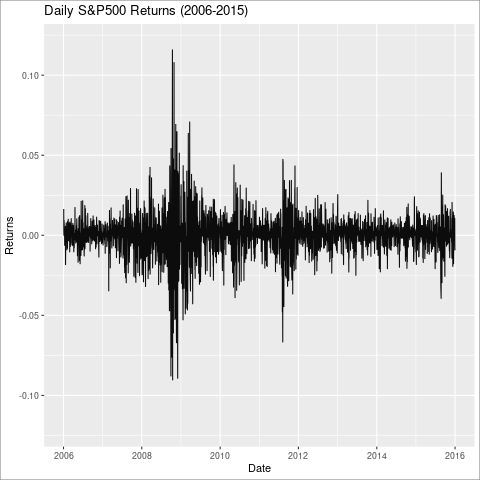
\includegraphics[scale=.45]{plot0615}
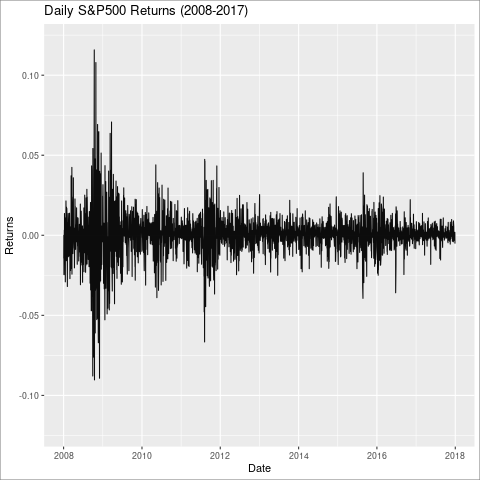
\includegraphics[scale=.45]{plot0817}
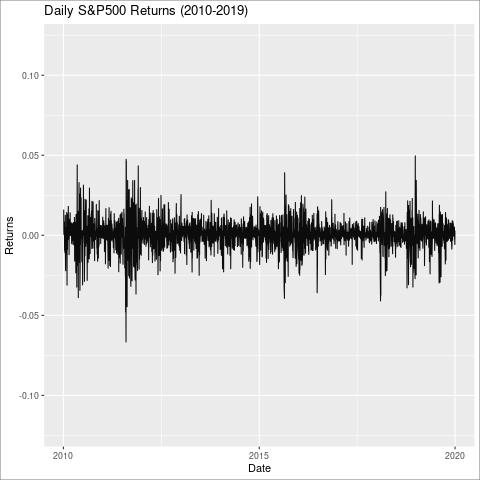
\includegraphics[scale=.45]{plot1019}
\caption{Training Data}
\end{figure}

Returns are normalized: they are calculated by taking the difference between the closing price for a day and the closing price for the previous day, and dividing it by the closing price of the previous day. The code for the data manipulation and setup is available in Appendix A.1. 
\begin{align}
Return_{t} = \frac{ClosingPrice_{t} - ClosingPrice_{t-1}}{ClosingPrice_{t-1}} \nonumber
\end{align}

The models are tested against data from the year immediately following the training period, that is, years 2016, 2018, and 2020. The 2016 test set has 252 observations with minimum -0.0359, maximum 0.0247, mean 0.0003, and standard deviation 0.0082. The 2018 test set has 251 observations with minimum -0.0409, maximum 0.0495, mean -0.0001, and standard deviation 0.0107. The 2020 test set has 253 observations with minimum -0.1198, maximum 0.0938, mean 0.0008, and standard deviation 0.0216. 

\begin{figure}
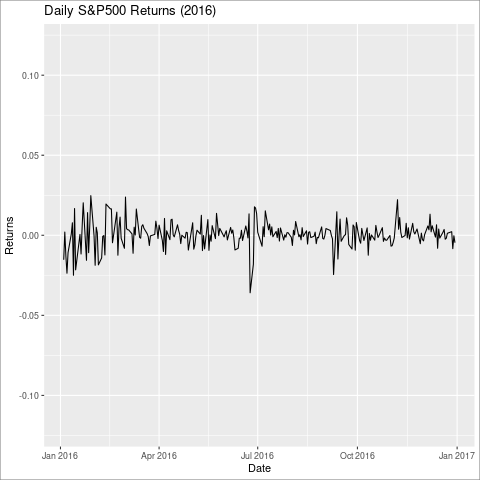
\includegraphics[scale=.5]{plot16}
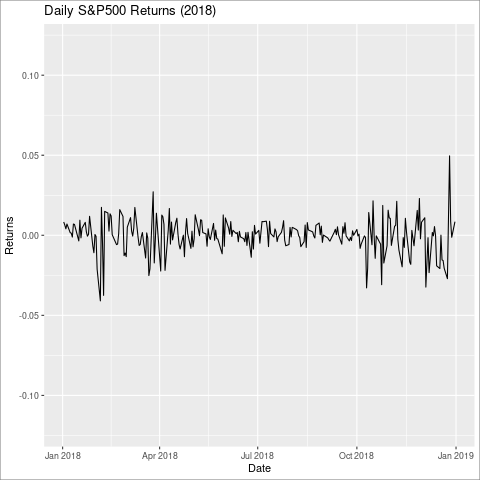
\includegraphics[scale=.5]{plot18}
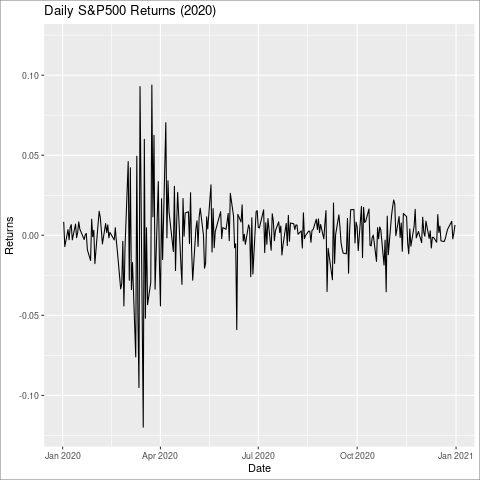
\includegraphics[scale=.5]{plot20}
\caption{Testing Data}
\end{figure}

\subsection{Models}
The two models are specified below. The Stan model codes are available in Appendix A.2. Both contain a log of volatility term, which is simply a transformation of variance.
\begin{align}
\lambda_t & = \ln(\sigma^2_t)
\implies \sigma_t = \exp(\lambda_t/2) 
\end{align}

\subsubsection{GARCH(1,1)}
The Generalized Autoregressive Conditional Heteroskedasticity model used here is specified below. This is a GARCH(1,1) model: it uses the return and volatility from one period prior to compute the volatility for the current period. Let $r_t$ denote the return at time $t$, which depends on $\mu$, the mean return, and $\lambda_t$, the log of volatility (variance) at time $t$. Furthermore, $\alpha_0$, $\alpha_1$, and $\beta_1$ are all positive, and $\alpha_1 + \beta_1 < 1$.  
\begin{align}
r_t &\sim Normal\bigl(\mu, \exp(\lambda_t/2)\bigr) \\
\mu &\sim Cauchy(0, 10) \\
\lambda_1 &\sim Cauchy(0,10) \\
\lambda_t &= \ln\bigl[\alpha_0 + \alpha_1 r_{t-1}^2 + \beta_1 \exp(\lambda_{t-1})\bigr] \\
\alpha_0  &\sim LogNormal(0,1) \\
\alpha_1 &\sim Uniform(0,1) \\
\beta_1 &\sim Uniform(0, 1 - \alpha_1)
\end{align}

The key parameters of the model are $\mu$, $\alpha_0$, $\alpha_1$, and $\beta_1$. These are used to predict $\lambda_t$, which is then used to estimate $r_t$. 

\subsubsection{Stochastic Volatility}
The Stochastic Volatility model is specified below. The return, $r_t$, depends on the mean, $\mu$, and log volatility, $\lambda_t = \ln(\sigma^2_t)$. Persistence of volatility is given by $\phi$, which is between -1 to 1, and the white noise scaling factor is given by $\tau$.

\begin{align}
r_t &\sim Normal\bigl(\mu, \exp({\lambda_t/2})\bigr) \\
\mu &\sim Cauchy(0, 10) \\
\lambda_1 &\sim Normal(\eta, \tau) \\
\lambda_t &\sim Normal\bigl(\eta + \phi(\lambda_{t-1} - \eta), \tau\bigr) \\
\eta &\sim Cauchy(0, 10) \\
\tau &\sim Cauchy(0, 10) \\
\phi &\sim Uniform(-1, 1)
\end{align}

The parameters of the model $\mu$, $\eta$, $\tau$, and $\phi$ are used to find $\lambda_t$, which is then used to estimate $r_t$. A key difference between the two approaches is that GARCH provides a deterministic representation of $\lambda_t$, whereas the Stochastic Volatility model provides, as the name suggests, a stochastic representation of $\lambda_t$.

Both models are coded in the probabilistic programming language Stan, which uses the adaptive variant of Hamiltonian Monte Carlo (HMC) called the No U-Turn Sampler (NUTS) proposed by Hoffman \& Gelman [2014]. Stan is designed to facilitate Bayesian inference for continuous-variable models using Monte Carlo methods [Carpenter et al., 2017].

\subsection{Hamiltonian Monte Carlo | Motivation}
Questions in statistics such as calculating means, medians, variance, and other higher moments involve computing expectations, which necessarily require solving some integration problem. Simple integrals have analytical solutions; but, often we need to integrate over complex distributions, and these integrals do not yield to closed forms. Markov Chain Monte Carlo (MCMC) methods are often used in these instances to derive sampling distibutions, which can then be used to approximate the required integrals.

MCMC algorithms typically use some transition operator satisfying the reversibility condition to move through the space of possible points from the target distribution. The operator specifies the transition probabilities between two points in the distribution. The algorithm is used to take a point $\theta_{previous}$ to the next point $\theta_{current}$, which is then appended to the Markov Chain. The algorithm is repeated multiple times, each time appending a point to the chain. The reversibility condition guarantees that the chain will eventually reach a stationary distribution, and beyond that, the chain, as it grows, will continue to remain within the stationary distribution. This stationary distribution is the target distribution (by design of the transition operator). Thus, as the chain grows longer, the values of the points in the chain begin to approximate the target distribution.

Different MCMC techniques exist for exploring the target distribution. Common MCMC methods include Random Walk Metropolis Sampling (RWMS) and Gibbs Sampling. These algorithms are simple to implement, however, in high dimesional parameter spaces with correlated parameters, RWMS and Gibbs Sampling prove to be inefficient as they make too many poor proposals (proposals that are accepted but too close to the current parameter value, or those that are distant from the current parameter value but from regions with low or no probability mass and hence rejected). In these cases, RWMS and Gibbs Sampling would require the Markov Chains to be inordinately long to sufficiently explore the regions of the target distribution where the probability mass is concentrated, and achieving this length would be computationally prohibitive. If, on the other hand, to make the chain computationally manageable, the algorithm is stopped before sufficient exploration, the expectations derived from the samples would be severely biased.

In high dimensional parameter spaces that are continuous and differentiable (as is the case with the two models specified above), Hamiltonian Monte Carlo (HMC) provides a solution to this exploration issue. The HMC Markov Chains are very efficient as consecutive points in each chain tend to be both far apart in the parameter space and from regions with high probability mass. The presence of high correlation between parameters does not hinder the exploration process of this MCMC algorithm. And while the generation of each new point in the sampling distribution involves more computation than in RWMS or Gibbs Sampling, many fewer points need to be generated to sufficiently cover the target space, leading to overall computational savings [Neal, 2011; Betancourt, 2017].

The general idea for HMC is as follows. We augment the $b$-dimensional parameter space with another set of $b$ auxiliary variables, one for each parameter. In this augmented $2b$-dimensional parameter space, the algorithm traverses from one point to another by following a long trajectory governed by Hamiltonian dynamics. This new point is then projected down to the original $b$-dimensional parameter space. The projected point is located in a region of high probability mass within the original parameter space, and yet is far away from the projection of the point that began the trajectory. This process is repeated and an efficient representative sample in the $b$-dimensional parameter space is derived [Neal, 2011; Betancourt, 2017]. 

\subsection{Hamiltonian Monte Carlo | Method}
For the GARCH model, $\theta = (\mu, \alpha_0, \alpha_1, \beta_1, \lambda_1, \lambda_2, ... , \lambda_T)$ where $T$ is the number of days in the training set for which we have a return value. Here, the dimension of the parameter space is $b = 4 + T$. 

Likewise, for the Stochastic Volatility model, $\theta = (\mu, \eta, \tau, \phi, \lambda_1, \lambda_2, ... , \lambda_T)$ where $T$ is the number of days in the training set for which we have a return value. Again, the dimension of the parameter space is $b = 4 + T$.

Details of the Hamiltonian Monte Carlo algorithm that follow are adaped from Neal [2011] and Betancourt [2017]. The HMC algorithm requires us to provide two functions: the natural logarithm of the joint distribution of the parameters, $\ln\pi(\theta)$, and the gradient of this function in all directions, $\frac{\partial \ln\pi(\theta)}{\partial \theta}$. This gradient (upon some modification) will guide the trajectory of the exploration. The subsequent steps in the HMC algorithm are as follows.

\begin{enumerate}
\item We augment $\theta$ with auxiliary variables $m$. Each parameter in $\theta$ has a corresponding auxiliary variable. Thus, $Dim(\theta) = Dim(m)$, say $b$. The augmented parameter space, $(\theta, m)$ is $2b$-dimensional. It is in this extended space that the algorithm will traverse.
\item Next, we define the Hamiltonian function, $H(\theta, m)$ as the negative of the natural logarithm of the joint density of the parameters and the auxiliary variables, that is, the augmented parameter space.
\begin{align}
H(\theta, m) \coloneqq - \ln \pi(\theta, m)
\end{align}
\item The Hamiltonian function decomposes as follows. 
\begin{align}
H(\theta, m) &= - \ln \pi(\theta, m) \\ \nonumber
&= - \ln [\pi(m | \theta). \pi(\theta)] \\ \nonumber
&= -\ln \pi(m | \theta) - \ln \pi(\theta)
\end{align}
Let $K(m, \theta) \coloneqq -\ln \pi(m | \theta)$ and $V(\theta) \coloneqq - \ln \pi(\theta)$. Note $V(\theta)$ follows from the specification of the target distribution. Any choice for the distribution of $\pi(m|\theta)$ would make the HMC valid. However, for simplicity and efficiency, the standard multivariate normal distribution is often chosen. Stan performs Euclidean HMC, which uses the standard multivariate normal distribution for $\pi(m|\theta)$ as well. 
\item The evolution of $\theta$ and $m$ is governed by the following Hamilton's equations.
\begin{align}
\frac{d\theta}{d\iota} &= \frac{\partial H(\theta, m)}{\partial m} \\ \nonumber
&= \frac{\partial[K(m, \theta) + V(\theta)]}{\partial m} \\ \nonumber
&= \frac{\partial K(m, \theta)}{\partial m}
\end{align}
\begin{align}
\frac{d m}{d \iota} &= - \frac{\partial H(\theta, m)}{\partial \theta} \\ \nonumber
&= - \frac{\partial[K(m, \theta) + V(\theta)]}{\partial \theta} \\ \nonumber
&= - \frac{\partial K(m, \theta)}{\partial \theta} - \frac{\partial V(\theta)}{\partial \theta}
\end{align}
Here $\iota$ is an imaginary time-step. $\frac{\partial V(\theta)}{\partial \theta}$ follows from the gradients provided to the HMC function. The differential equations in (31) and (32) together define a vector field, the contours of which align with the high mass regions in the parameter space. 
\end{enumerate}

Stan uses autodifferentiation [Carpenter et al., 2015] to construct the derivatives above. In addition to the two functions, the implementation of HMC in Stan requires two other quantities: stepsize and number of leapfrog steps. The stepsize governs the length of the imaginary time-step mentioned in step (4). The number of leapfrog steps governs how many imaginary time-steps forward the parameter is propagated in order to arrive at the new proposed parameter. 

In practice, depending on the terrain of the joint posterior, for certain values of stepsize and number of leapfrog steps, it is possible for the algorithm to generate trajectories that loop back to or near the starting point, and hence be inefficient. The right selection of stepsize and number of leapfrog steps is important for efficient exploration.

Stan uses the adaptive variant of HMC called the No U-Turn Sampler (NUTS) to avoid these inefficiencies. The NUTS algorithm uses iterations in the warmup period to automatically test various stepsizes and number of leapfrog steps and optimize these two quantitites [Carpenter et al., 2017].  

\subsection{Parameter Estimation}
For the GARCH model, 50,000 iterations are run on 4 chains each. 50\% of the iterations are used for warmup, resulting in a posterior sample of 100,000 points in total.  

For the Stochastic Volatility model, 1,000,000 iterations are run on 4 chains for 100,000 iterations each. Half of the iterations are used up in the warmup phase, and one out of 20 successive points is selected resulting again in 100,000 points from the posterior distribution. More iterations and thinning are used in this model to compensate for slower convergence and higher autocorrelation in parameters $\phi$ and $\tau$. 

The code used for fitting the models is available in Appendix A.3.

\subsection{Parameter Updates}
Updating parameters involves the Sequential Monte Carlo step of assigning weights to each of the 100,000 points from the posterior distribution and then resampling (with replacement) as many points according to these weights whenever the Effective Sample Size (ESS) drops under an acceptable threshold (set, here, at 0.9). Details of this method are listed in Capp\'{e} [2007].

The Effective Sample Size (ESS) quantifies the amount of independent information or effective data points in a sample. In Markov Chain Monte Carlo procedures (including Hamiltonian Monte Carlo, the procedure used in this paper), the goal is to generate a sequence of correlated samples from a target distribution to estimate various properties of interest. However, due to the inherent correlation between successive samples in the chains generated, the effective amount of independent information is typically lower than the actual sample size. The ESS is calculated as follows. 
\begin{align}
ESS = \frac{\text{N}}{1 + 2\sum_{t=1}^{\infty}\rho_t}
\end{align}
Where $N$ is the number of iterations, and $\rho_t$ is the autocorrelation corresponding to a lag of $t$ time units.

The weights are determined using the Gaussian density function on the predicted return at each point. That is, given the mean and standard deviation (a tansformation of lambda) corresponding to a point, the point will have a higher weight if the Gaussian density for its predicted return is higher, and vice versa. The weights are normalized by the sum of all the weights. Whenever, over the course of iterated propagation (described in section 3.8 below), the ESS falls below the specified threshold, the cloud of 100,000 points are resampled with replacement according to these normalized weights. 

Appendix A.4 provides the code for assigning weights and resampling.

\subsection{Prediction and Propagation}
Using the parameters found above, each point at time $t$ is used to predict the point at time $t+1$. Lambda at time $t+1$ is estimated first using the parameters at time $t$, and then $\lambda_{t+1}$ (along with other parameters) is used to generate return at time $t+1$. 

``Propagation" refers to moving the cloud of 100,000 points one step forward. Before each propagation, we check the effective sample size and resample if necessary. The  propagation is done for each month, each quarter, and for the whole year, for the years 2016, 2018, and 2020. 

Appendix A.4 contains the code for prediction and propagation.

\subsection{Performance Comparison}
After the predicted returns are calculated by both models for the three different time-frames, the results are tested against the returns data for 2016, 2018, and 2020 using the sum of squared errors. The empirical distributions of predictions are used to compute the fraction of the observed returns data that fall within the 2.5 percentile and the 97.5 percentile of the predicted returns.  

Appendix A.5 provides the performance comparison code. 

\newpage
\section{Results}

\subsection{GARCH Parameter Estimates}
Figures 1-3 below contain the histograms of the 100,000 point posterior samples generated from the GARCH model.

\subsubsection{2006-15}
\begin{figure}
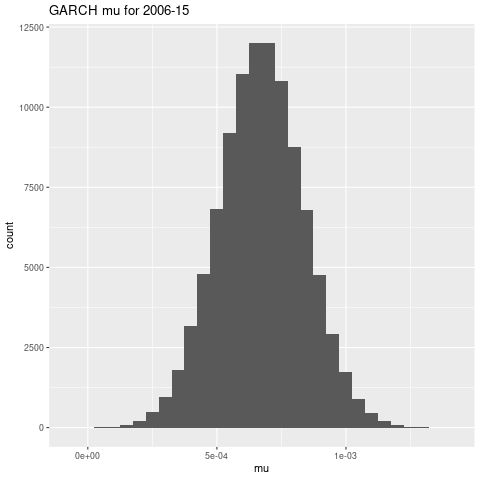
\includegraphics[scale = .4]{gmu0615}
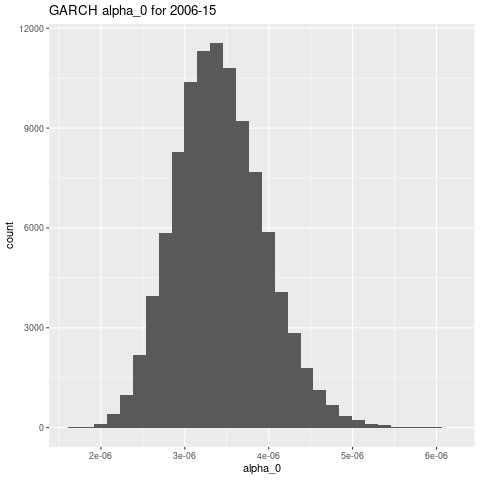
\includegraphics[scale = .4]{ga00615}
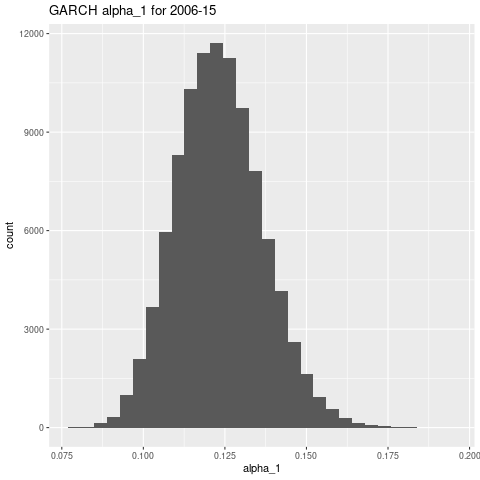
\includegraphics[scale = .4]{ga10615}
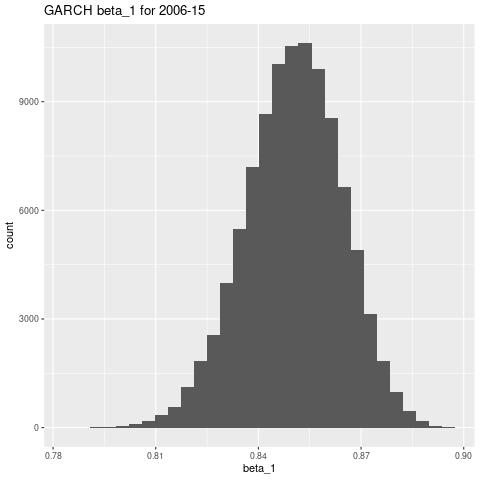
\includegraphics[scale = .4]{gb10615}
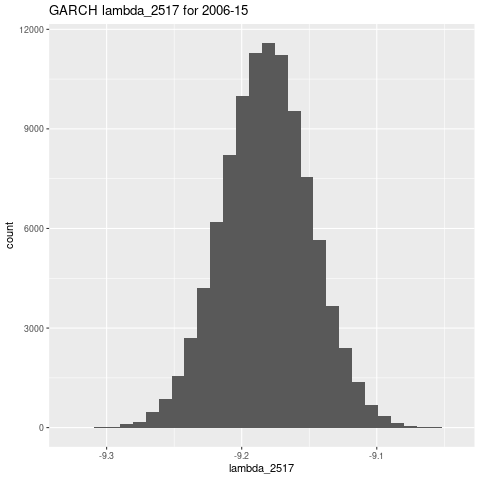
\includegraphics[scale = .4]{glT0615}
\caption{GARCH posterior samples for 2006-15 training data.}
\end{figure}

The mean estimates for the parameters are as follows.
\begin{align*}
\mu &= 0.0006 \\
\alpha_0 &= 0.0000 \\
\alpha_1 &= 0.1235 \\
\beta_1 &= 0.8502
\end{align*}

The lambda corresponding to the last time period in the training set has a mean of $-9.1817$.

\subsubsection{2008-17}
\begin{figure}
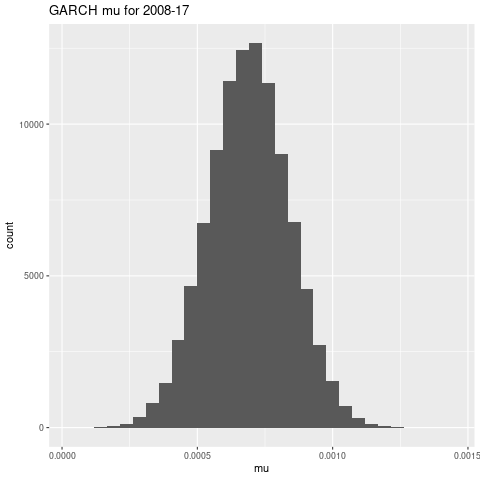
\includegraphics[scale = .4]{gmu0817}
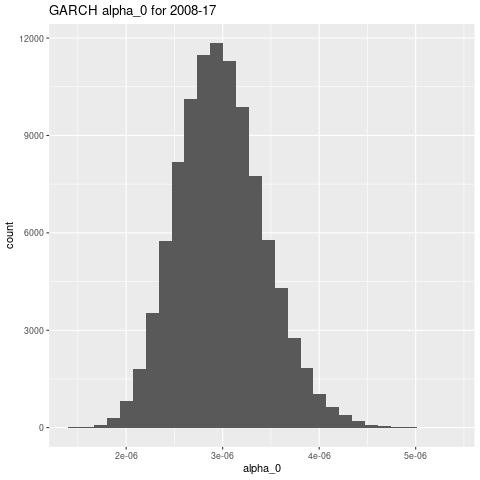
\includegraphics[scale = .4]{ga00817}
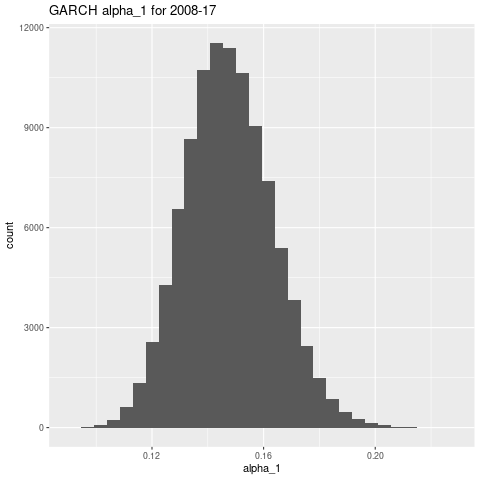
\includegraphics[scale = .4]{ga10817}
\includegraphics[scale = .4]{gb10817}
\includegraphics[scale = .4]{glT0817}
\caption{GARCH posterior samples for 2008-17 training data.}
\end{figure}

The mean estimates for the parameters are as follows.
\begin{align*}
\mu &= 0.0006 \\ 
\alpha_0 &= 0.0000 \\ 
\alpha_1 &= 0.1475 \\ 
\beta_1 &= 0.8300 
\end{align*}

The lambda corresponding to the last time period in the training set has a mean of $-10.6268$.

\subsubsection{2010-19}
\begin{figure}
\includegraphics[scale = .4]{gmu1019}
\includegraphics[scale = .4]{ga01019}
\includegraphics[scale = .4]{ga11019}
\includegraphics[scale = .4]{gb11019}
\includegraphics[scale = .4]{glT1019}
\caption{GARCH posterior samples for 2010-19 training data.}
\end{figure}

The mean estimates for the parameters are as follows.
\begin{align*}
\mu &= 0.0008 \\ 
\alpha_0 &= 0.0000 \\ 
\alpha_1 &= 0.1871 \\ 
\beta_1 &= 0.7621 
\end{align*}

The lambda corresponding to the last time period in the training set has a mean of $-10.3061$.

\subsection{Stochastic Volatility Parameter Estimates}
The histograms of the 100,000 point posterior samples generated from the Stochastic Volatility model are as follows.

\subsubsection{2006-15}
\begin{figure}
\includegraphics[scale = .4]{svmu0615}
\includegraphics[scale = .4]{sve0615}
\includegraphics[scale = .4]{svp0615}
\includegraphics[scale = .4]{svt0615}
\includegraphics[scale = .4]{svlT0615}
\caption{Stochastic Volatility posterior samples for 2006-15 training data.}
\end{figure}

The Stochastic Volatility parameter estimates using mean values are below in figures 4-6.
\begin{align*}
\mu &= 0.0008 \\
\eta &= -9.4503 \\
\phi &= 0.9798 \\
\tau &= 0.2190 
\end{align*}

The lambda corresponding to the last time period in the training set has a mean of $-9.2065$.

\subsubsection{2008-17}
\begin{figure}
\includegraphics[scale = .4]{svmu0817}
\includegraphics[scale = .4]{sve0817}
\includegraphics[scale = .4]{svp0817}
\includegraphics[scale = .4]{svt0817}
\includegraphics[scale = .4]{svlT0817}
\caption{Stochastic Volatility posterior samples for 2008-17 training data.}
\end{figure}

The Stochastic Volatility parameter estimates using mean values are below in figures 4-6.
\begin{align*}
\mu &= 0.0008 \\
\eta &= -9.3779 \\
\phi &= 0.9785 \\
\tau &= 0.2560
\end{align*}

The lambda corresponding to the last time period in the training set has a mean of $-11.0425$.

\subsubsection{2010-19}
\begin{figure}
\includegraphics[scale = .4]{svmu1019}
\includegraphics[scale = .4]{sve1019}
\includegraphics[scale = .4]{svp1019}
\includegraphics[scale = .4]{svt1019}
\includegraphics[scale = .4]{svlT1019}
\caption{Stochastic Volatility posterior samples for 2010-19 training data.}
\end{figure}

The Stochastic Volatility parameter estimates using mean values are below in figures 4-6.
\begin{align*}
\mu &= 0.0009 \\
\eta &= -9.8949 \\
\phi &= 0.9469 \\
\tau &= 0.3366
\end{align*}

The lambda corresponding to the last time period in the training set has a mean of $-10.8228$.

\subsection{Comparing Sum of Squared Errors of Estimated Returns}
The parameter estimates obtained above for the GARCH and the Stochastic Volatility models are used to (a) estimate the hidden variable, lambda, and (b) predict the return, for the next time step. This is done for the entire cloud of 100,000 points. Then, the parameters are updated using the parameter update step described above. Next, the estimation of lambda and prediction of return for the subsequent time step are done. The execution details are in Appendix A.4.

The code in Appendix A.4 generates predictions for the years 2016 (a low volatility year), 2018 (medium volatility year) and 2020 (a high volatility year). These predictions are compared against the test data from 2016, 2018 and 2020 using sum of squared errors. Appendix A.5 contains the corresponding comparison code. Tables 1-3 present the SSE for the two models for the three years along with an indicator for which model has the lower SSE.

\begin{table}[!ht]
    \centering
    \begin{tabular}{|l|l|l|l|}
    \hline
        ~ & \textbf{GARCH} & \textbf{SV} & \textbf{Result} \\ \hline
        \textbf{Month 1 }& 0.0047 & 0.0047 & Equal \\ \hline
        \textbf{Month 2} & 0.0027 & 0.0027 & Equal \\ \hline
        \textbf{Month 3} & 0.0006 & 0.0006 & Equal \\ \hline
        \textbf{Month 4} & 0.0009 & 0.0009 & Equal \\ \hline
       \textbf{Month 5} & 0.0008 & 0.0008 & Equal \\ \hline
       \textbf{Month 6} & 0.0028 & 0.0028 & Equal \\ \hline
        \textbf{Month 7} & 0.0004 & 0.0004 & Equal \\ \hline
        \textbf{Month 8} & 0.0002 & 0.0002 & Equal \\ \hline
        \textbf{Month 9} & 0.0016 & 0.0016 & Equal \\ \hline
        \textbf{Month 10} & 0.0003 & 0.0003 & Equal \\ \hline
        \textbf{Month 11} & 0.0009 & 0.0009 & Equal \\ \hline
        \textbf{Month 12} & 0.0005 & 0.0005 & Equal \\ \hline
        \textbf{Quarter 1} & 0.0082 & 0.0082 & Equal \\ \hline
        \textbf{Quarter 2} & 0.0046 & 0.0046 & Equal \\ \hline
        \textbf{Quarter 3} & 0.0024 & 0.0024 & Equal \\ \hline
        \textbf{Quarter 4} & 0.0018 & 0.0018 & Equal \\ \hline
        \textbf{Full Year} & 0.0171 & 0.0171 & Equal \\ \hline
    \end{tabular}
\caption{Sum of Squared Errors for 2016}
\end{table}

\begin{table}[!ht]
    \centering
    \begin{tabular}{|l|l|l|l|}
    \hline
        ~ & \textbf{GARCH} & \textbf{SV} & \textbf{Result} \\ \hline
        \textbf{Month 1} & 0.0007 & 0.0007 & Equal \\ \hline
        \textbf{Month 2} & 0.0056 & 0.0056 & Equal \\ \hline
        \textbf{Month 3} & 0.0037 & 0.0037 & Equal \\ \hline
        \textbf{Month 4} & 0.0017 & 0.0017 & Equal \\ \hline
        \textbf{Month 5} & 0.0009 & 0.0009 & Equal \\ \hline
        \textbf{Month 6} & 0.0005 & 0.0005 & Equal \\ \hline
        \textbf{Month 7} & 0.0006 & 0.0006 & Equal \\ \hline
        \textbf{Month 8} & 0.0004 & 0.0004 & Equal \\ \hline
        \textbf{Month 9} & 0.0002 & 0.0002 & Equal \\ \hline
        \textbf{Month 10} & 0.0045 & 0.0045 & Equal \\ \hline
        \textbf{Month 11} & 0.0028 & 0.0028 & Equal \\ \hline
        \textbf{Month 12} & 0.0069 & 0.0069 & Equal \\ \hline
        \textbf{Quarter 1} & 0.0100 & 0.0100 & Equal \\ \hline
        \textbf{Quarter 2} & 0.0032 & 0.0032 & Equal \\ \hline
        \textbf{Quarter 3} & 0.0012 & 0.0012 & Equal \\ \hline
        \textbf{Quarter 4} & 0.0144 & 0.0144 & Equal \\ \hline
        \textbf{Full Year} & 0.0290 & 0.0290 & Equal \\ \hline
    \end{tabular}
\caption{Sum of Squared Errors for 2018}
\end{table}

\begin{table}[!ht]
    \centering
    \begin{tabular}{|l|l|l|l|}
    \hline
        ~ & \textbf{GARCH} & \textbf{SV} & \textbf{Result} \\ \hline
        \textbf{Month 1} & 0.0011 & 0.0011 & Equal \\ \hline
        \textbf{Month 2} & 0.0078 & 0.0078 & Equal \\ \hline
        \textbf{Month 3} & 0.0724 & 0.0724 & Equal \\ \hline
        \textbf{Month 4} & 0.0129 & 0.0129 & Equal \\ \hline
        \textbf{Month 5} & 0.0032 & 0.0032 & Equal \\ \hline
        \textbf{Month 6} & 0.0071 & 0.0071 & Equal \\ \hline
        \textbf{Month 7} & 0.0015 & 0.0015 & Equal \\ \hline
        \textbf{Month 8} & 0.0006 & 0.0006 & Equal \\ \hline
        \textbf{Month 9} & 0.0049 & 0.0049 & Equal \\ \hline
        \textbf{Month 10} & 0.0035 & 0.0035 & Equal \\ \hline
        \textbf{Month 11} & 0.0025 & 0.0025 & Equal \\ \hline
        \textbf{Month 12} & 0.0006 & 0.0005 & SV is lower \\ \hline
        \textbf{Quarter 1} & 0.0814 & 0.0813 & SV is lower \\ \hline
        \textbf{Quarter 2} & 0.0233 & 0.0233 & Equal \\ \hline
        \textbf{Quarter 3} & 0.0071 & 0.0071 & Equal \\ \hline
        \textbf{Quarter 4} & 0.0066 & 0.0066 & Equal \\ \hline
        \textbf{Full Year} & 0.1185 & 0.1185 & Equal \\ \hline
    \end{tabular}
\caption{Sum of Squared Errors for 2020}
\end{table}

\newpage
\subsection{Comparing Capture in 95 Percent Band}
The empirical distributions of the predicted returns for 2016, 2018, and 2020 are used to find the predictions at the 2.5 percentile and the 97.5 percentile for both models in each day of the three years. For the GARCH model, the 95 percent prediction band captured 238 out of 252 observations in 2016; 243 out of 251 observations in 2018; and 206 out of 253 observations in 2020. 
For the Stochastic Volatility model, the 95 percent prediction band captured 237 out of 252 observations in 2016; 242 out of 251 observations in 2018; and 203 out of 253 observations in 2020. The corresponding code is in Appendix A.5.

\newpage
\section{Discussion}
In terms of SSE, both models perform nearly identically across all time-frames and in all three time periods. Small differences in the sum of squared errors arise, usually, in the ten-thousandths place or later. These small differences can be attributed to the monte carlo errors associated with the computations. 

Out of the twelve month long time-frames assessed for 2016, the GARCH and the Stochastic Volatility results are indistinguishable in every month. These SSEs range from a low of 0.0002 to a high of 0.0047 for both estimates. The highs and the lows occur on the same months for both the models.

Out of the twelve month long time-frames assessed for 2018, the GARCH and the Stochastic Volatility results are indistinguishable in every month. These SSEs range from a low of 0.0002 to a high of 0.0069 for the both estimates. The highs and the lows occur on the same months for both the models.

Out of the twelve month long time-frames assessed for 2020, the GARCH results are indistinguishable from the Stochastic Volatility results on 11 occasions. The only small noticeable difference occur in month 12, for which the Stochastic Volatility estimate shows a lower sum. These SSEs range from a low of 0.0006 to a high of 0.0724 for the GARCH estimates, while for the Stochastic Volatility estimates, they range from a low of 0.0005 to a high of 0.0724. The highs and the lows occur on the same months for both the models.

Out of the four quarters assessed for 2016, GARCH and Stochastic Volatility perform equally well in every quarter. These SSEs range from a low of 0.0018 to a high of 0.0082 for both estimates. The highs and the lows for both models occur in the same quarters.  

Out of the four quarters assessed for 2018, GARCH and Stochastic Volatility perform equally well in every quarter. These SSEs range from a low of 0.0012 to a high of 0.0144 for both estimates. The highs and the lows for both models occur in the same quarters.

Out of the four quarters assessed for 2020, GARCH and Stochastic Volatility are indistinguishable in every quarter except the first. In quarter 1, the sum for Stochastic Volatility is slightly lower. The SSEs range from a low of 0.0066 to a high of 0.0814 for the GARCH estimates, while for the Stochastic Volatility estimates, they range from a low of 0.0066 to a high of 0.0813. The highs and the lows for both models occur in the same quarters.  

For every full year assessed, the GARCH and the Stochastic Volatility models deliver identical results. For 2016, the full-year SSE is 0.0171. For 2018, the full-year SSE is 0.0290. For 2020, despite small differences in monthly or quarterly results, the full-year SSE is 0.1185 for both models. 

In general, we notice that the models have the least SSE in the low volatility year (2016) and the highest SSE in the high volatility year (2020).
The differences in the predictive performance between the two models are not practically significant. When one model has low SSE, the other model has low SSE too, and when one has high SSE, the other shows similar effect. The small differences that arise can be attributed to the randomness involved in the prediction process. 

The 95 percent prediction bands perform similarly for both models as well. In 2016, the prediction bands for the GARCH model capture 238 out of 252 observations (94.44\% accuracy) while those for the Stochastic Volatility model capture 237 out of 252 observations (94.04\% accuracy). In 2018, they capture 243 out of 251 observations (96.81\% accuracy) for GARCH, and 242 out of 251 observations for Stochastic Volatility (96.41\% accuracy). Finally, in 2020, they capture 206 out of 253 observations for GARCH (81.42\% accuracy), and 203 out of 253 observations for Stochastic Volatility (80.23\% accuracy). While the GARCH model is slightly more predictive in each year above, they differ by only one day. Also, in the high-volatility year of 2020, the predictive accuracy of both models reduce significantly. Hence, in practical terms, both models are indistinguishable. 


\newpage
\section{Further Studies}
This paper uses various ten-year daily returns of the S\&P-500 Index from 2006 to 2020 to make parameter estimates and predictions. Sections 4.1 and 4.2 provide the distributions of the parameter estimates for the GARCH and Stochastic Volatility models, but immediately reduce the results to point estimates for subsequent analysis. The distributions themselves remain under-explored. Further studies might take into account the full distributions of these parameters for generating predictions. 

The compression of distribution-based outputs to single points can be seen again in section 4.3 where the computation of SSE necessitates the use of the mean of the daily predicted return values. This has the effect of producing results nearly identical to those obtained simply by computing SSEs with the fixed $\mu$s generated by each HMC simulation but at significantly higher computational costs. While section 4.4 makes use of the empirical distribution of the predictions to ascertain whether the observations fall within the 2.5 percentile and the 97.5 percentile of predicted returns for each day of the test years, the distribution properties of the predictions remain under-utilized. 

Further study could include an analysis of distribution-based properties such as the width of the prediction bands and the thickness of the tails. For instance, the outputs of the Stochastic Volatility models generally result in greater kurtosis in all three test years. (In 2016, the skewness of the distribution of kurtosis of the daily predicted returns for the GARCH model is 0.1964 as opposed to 1.0573 for the Stochastic Volatility model. This implies that the kurtosis of daily returns is more right-skewed for the Stochastic Volatility model, further implying that the distribution of predicted returns from the Stochastic Volatility model is thicker-tailed. This result holds for 2018 with the skewness of the kurtosis at 1.0021 for GARCH and 4.8058 for Stochastic Volatility; and for 2020 with the skewness of kurtosis at 1.9687 and 4.4532 for GARCH and Stochastic Volatility respectively. Appendix A.5 contains the corresponding code to generate these results.) An exploration of  the process resulting in these differences and their implications might be of interest, especially when the analysis is done from a risk-management/ruin-avoidance framework (as in Taleb [2020]) rather than a prediction-oriented framework.

Probabilistic forecasting is another approach that may be taken to make claims about the returns predictions. In this case, probabilistic forecasting would generate various ranges of returns and the associated probabilities for observing returns in those ranges. Gneiting \& Katzfuss [2014] describes the method of probabilistic forecasting in further details.

Certain parameters of the models, namely, $\mu$ and $\lambda_1$ for GARCH, and $\mu$, $\eta$, and $\tau$ for Stochastic Volatility begin with noninformative $Cauchy(0,10)$ priors. While this lack of previous information allows for a derivation of the distributions solely based on the training data, the convergence can be vastly sped up by the use of informative priors. The posterior sampling distributions generated in this paper may be used to generate priors in future studies.

Moreover, the methodology used in this paper may also be used on assets other than the S\&P-500 Index. It would be interesting to see how different the results are and whether the prediction accuracy holds for the other assets.

Finally, an aspect of modeling this paper does not cover is computation time. In this study, the parameter estimation for Stochastic Volatility took several times as long as the parameter estimation for GARCH, and yet resulted in similar outputs. Further studies could involve more optimization of the code, closer monitoring of the estimation and prediction times, and use of other software.   

\newpage

\appendix
\section{Codes}

\subsection{Data Preparation and Exploration}
\begin{verbatim}

library(here)
library(tidyverse)
library(vroom) 
library(lubridate)
library(ggplot2)
library(ggthemes)

data = vroom(here("SPX_from_2000_to_2022.csv"))

data = data %>%
  mutate(Date = mdy(Date)) %>%
  arrange(Date) %>%
  mutate(Returns = (Close - lag(Close))/lag(Close)) %>%
  select(c(Date, Returns)) 

data0615 = data %>% filter(Date > "2005-12-31" & Date < "2016-01-01")
data16 = data %>% filter(Date > "2015-12-31" & Date < "2017-01-01")

data0817 = data %>% filter(Date > "2007-12-31" & Date < "2018-01-01")
data18 = data %>% filter(Date > "2017-12-31" & Date < "2019-01-01")

data1019 = data %>% filter(Date > "2009-12-31" & Date < "2020-01-01")
data20 = data %>% filter(Date > "2019-12-31" & Date < "2021-01-01")


png("plot0615.png")
ggplot(data0615, aes(x=Date, y=Returns)) +
  geom_point(alpha=0.25, color = "black") +
  scale_x_date() +
  ylim(-0.12, 0.12) +
  theme(plot.background = element_rect(colour = "grey50")) +
  ggtitle("Daily S&P500 Returns (2006-2015)")
dev.off

png("plot16.png")
ggplot(data16, aes(x=Date, y=Returns)) +
  geom_line(color = "black") +
  scale_x_date() +
  ylim(-0.12, 0.12) +
  theme(plot.background = element_rect(colour = "grey50")) +
  ggtitle("Daily S&P500 Returns (2016)")
dev.off

#repeat for other years

\end{verbatim}

\subsection{Stan Models}
\begin{verbatim}

# install.packages("rstan", 
# repos = "https://cloud.r-project.org", dependencies=TRUE)
library(rstan)

# Stan Models

# GARCH Model:
model_G <- "data {
  int<lower=0> T;
  real r[T];
}
parameters {
  real mu;
  real<lower=0> alpha0;
  real<lower=0, upper=1> alpha1;
  real<lower=0, upper=(1-alpha1)> beta1;
  real lambda1;
}
transformed parameters {
  real lambda[T];
  lambda[1] = lambda1;
  for (t in 2:T) {
    lambda[t] = log(alpha0
                     + alpha1 * pow((r[t - 1] - mu), 2)
                     + beta1 * exp(lambda[t - 1]));
  }
}
model {
  for (t in 1:T) {
    r[t] ~ normal(mu, exp(lambda[t]/2));
  }
  lambda1 ~ cauchy(0,10); 
  alpha0 ~ lognormal(0,1);
  alpha1 ~ uniform(0,1);
  beta1 ~ uniform(0, 1 - alpha1);
  mu ~ cauchy(0, 10);
}"

# Stochastic Volatility Model:
model_SV <- "data {
  int<lower=0> T;   
  real r[T];      
}
parameters {
  real mu;                     
  real eta;
  real<lower=-1, upper=1> phi; 
  real<lower=0> tau;         
  real lambda[T];                
}
model {
  phi ~ cauchy(0, 10);
  tau ~ cauchy(0, 10);
  mu ~ cauchy(0, 10);
  eta ~ cauchy(0, 10);
  lambda[1] ~ normal(eta, tau);
  for (t in 2:T) {
    lambda[t] ~ normal(eta + phi * (lambda[t - 1] -  eta), tau);
  }
  for (t in 1:T) {
    r[t] ~ normal(mu, exp(lambda[t] / 2));
  }
}
"

\end{verbatim}

\subsection{Fitting}
\begin{verbatim}
set.seed(2023)

#libraries
# install.packages("rstan", repos = "https://cloud.r-project.org", 
# dependencies=TRUE)
library(rstan)

data = data0615 # or data0817,1019 as appropriate
len = nrow(data)

# Model Fitting
# The following will generate 100,000 points each.

# GARCH
st_G = Sys.time()
fit_G <- stan(model_code = model_G, data = list(T = len, r = data$Returns), 
iter = 50000, chains = 4, cores = 4)
ed_G = Sys.time()
tt_G = ed_G - st_G

# Stochastic Volatility
st_SV = Sys.time()
fit_SV <- stan(model_code = model_SV, data = list(T = len, r = data$Returns), 
iter = 1000000, chains = 4, cores = 4, thin = 20)
ed_SV = Sys.time()
tt_SV = ed_SV - st_SV

# Saving results (Rename accordingly with 0615, 0817, or 1019)
saveRDS(fit_G, file='fit_G0615.rds')
saveRDS(fit_SV, file='fit_SV0615.rds') 

# Extracting Parameters
parameters_G = extract(fit_G)   # contains mu, alpha0, alpha1, beta1, lambdas
parameters_SV = extract(fit_SV) # contains mu, eta, tau, phi, lambdas

\end{verbatim}

\subsection{Prediction}
\begin{verbatim}

set.seed(2023)

#libraries
library(here)
library(tidyverse)
library(lubridate)
library(ggplot2)
library(ggthemes)
# install.packages("rstan", repos = "https://cloud.r-project.org", 
# dependencies=TRUE)
library(rstan)


# Select appropriate dataset
data = data18

# Read appropriate fit file, 0615, 0817, or 1019
fit_G = readRDS(file = "fit_G0817.rds")
fit_SV = readRDS(file = "fit_SV0817.rds")

# Parameter extraction
parameters_G = extract(fit_G)   # contains mu, alpha0, alpha1, beta1, lambdas
parameters_SV = extract(fit_SV) # contains mu, eta, phi, tau, lambdas



# Creating initial dataframe

df_G = data.frame("mu" = parameters_G$mu, "alpha0" = parameters_G$alpha0,
"alpha1" = parameters_G$alpha1,"beta1"=parameters_G$beta1, 
"lambda_t" = parameters_G$lambda[,nrow(data)])

df_SV = data.frame("mu" = parameters_SV$mu, "eta" = parameters_SV$eta,
"phi" = parameters_SV$phi, "tau"= parameters_SV$tau, 
"lambda_t" = parameters_SV$lambda[,nrow(data)])

pred_returns_G = mapply(function(mean, sd) {rnorm(1, mean, sd)}, df_G$mu,
exp(df_G$lambda_t/2))

pred_returns_SV = mapply(function(mean, sd) {rnorm(1, mean, sd)},
df_SV$mu, exp(df_SV$lambda_t/2))
### this has the same effect as
###for (i in 1:nrow(df_G)) {
###  pred_returns[i] = rnorm(1, mean=df_G$mu[i], sd=exp(df_G$lambda_t[i] / 2))
###}

df_G = cbind(df_G, "pred_returns" = pred_returns_G)
df_SV = cbind(df_SV, "pred_returns" = pred_returns_SV)



# Assigning Weights

Weights_G = function(df_G){
  # takes df with garch parameters and pred_returns, outputs normalized weights
  weights = mapply(function(return, mean, sd) {dnorm(return, mean, sd)}, 
                   df_G$pred_returns, df_G$mu, exp(df_G$lambda_t / 2))
  weights = weights / sum(weights)
  return(weights)
}

Weights_SV = function(df_SV){
  # takes df with SV parameters and pred_returns, outputs normalized weights
  weights = mapply(function(return, mean, sd) {dnorm(return, mean, sd)}, 
                   df_SV$pred_returns, df_SV$mu, exp(df_SV$lambda_t / 2))
  weights = weights / sum(weights)
  return(weights)
}


# Effective Sample Size
# = Number of Iterations / (1 + sum of Autocorrelations from lag 1 to infinity)
#ess = nrow(df) / (1 + 2*(sum(acf(df$lambda_t, plot = FALSE)$acf)-1))

# Resampling

Resample = function(df, weights) {
  ess = nrow(df) / (1 + 2*(sum(acf(df$lambda_t, plot = FALSE)$acf)-1))
  threshold = .9
  if (ess < threshold*nrow(df)) {
    new_df = df[sample(seq_len(nrow(df)), nrow(df), 
    replace = TRUE, prob = weights), ]
    print("resampled")
    return(new_df)    
  } else {
    print("same sample")
    return(df)
  }
}


# Point parameter estimates for the GARCH model
mu_G = mean(parameters_G$mu)
alpha0 = mean(parameters_G$alpha0)
alpha1 = mean(parameters_G$alpha1)
beta1 = mean(parameters_G$beta1)
lambdaT_G = mean(parameters_G$lambda[,ncol(parameters_G$lambda)])

# Point parameter estimates for the Stochastic Volatility model
mu_SV = mean(parameters_SV$mu)
eta = mean(parameters_SV$eta)
phi = mean(parameters_SV$phi)
tau = mean(parameters_SV$tau)
lambdaT_SV = parameters_SV$lambda[,ncol(parameters_G$lambda)]


# Prediction and Propagation
# (prediction: single point 1 step forward,
#  propagation: n points 1 step forward    )

Predict_G = function(prev_lambda, prev_return){
  pred_lambda = log(alpha0
                     + alpha1 * ((prev_return - mu_G)^2)
                     + beta1 * exp(prev_lambda))
  pred_return = rnorm(1, mean=mu_G, sd=exp(pred_lambda / 2))
  return(c("pred_lambda" = pred_lambda, "pred_return" = pred_return))
}

Predict_SV = function(prev_lambda){
  pred_lambda = rnorm(1, eta + phi * (prev_lambda - eta), tau)
  pred_return = rnorm(1, mean = mu_SV, exp(pred_lambda/2))
  return(c("pred_lambda" = pred_lambda, "pred_return" = pred_return))
}

Propagate_G = function(df) {
  new_df = df
  for (i in 1:nrow(new_df)){
    result = Predict_G(df$lambda_t[i], df$pred_returns[i])
    new_df$lambda_t[i] = result[1]
    new_df$pred_returns[i] = result[2]
  }
  return(new_df)
}

Propagate_SV = function(df) {
  new_df = df
  for (i in 1:nrow(new_df)){
    result = Predict_SV(df$lambda_t[i])
    new_df$lambda_t[i] = result[1]
    new_df$pred_returns[i] = result[2]
  }
  return(new_df)
}


# Execution

T = nrow(data) # time steps (select appropriate year)

# SMC Propagation with Resampling
# df_G and df_SV are the initial inputs

list_G = list(df_G)
df = df_G
st_G = Sys.time()
for (t in 1:T) {
  df = Resample(df, weights = Weights_G(df))
  
  mu_G <<- mean(df$mu)
  alpha0 <<- mean(df$alpha0)
  alpha1 <<- mean(df$alpha1)
  beta1 <<- mean(df$beta1)
  lambdaT_G <<- mean(df$lambda_t)

  df = Propagate_G(df)
  list_G = append(list_G, list(df))
}
ed_G = Sys.time()
tt_G = ed_G - st_G

list_SV = list(df_SV)
df = df_SV
st_SV = Sys.time()
for (t in 1:T) {
  df = Resample(df, weights = Weights_SV(df))
  
  mu_SV <<- mean(df$mu)
  eta <<- mean(df$eta)
  phi <<- mean(df$phi)
  tau <<- mean(df$tau)
  lambdaT_SV <<- mean(df$lambda_t)

  df = Propagate_G(df)
  list_SV = append(list_SV, list(df))
}
ed_SV = Sys.time()
tt_SV = ed_SV - st_SV

saveRDS(list_G, file='list_G18.rds') 
saveRDS(list_SV, file='list_SV18.rds')

#list_G and list_SV will contain the predicted returns (inter alia)
#for each time step. These lists contain one too many elements. 
#The prediction begins from the second element on.

# Save lists with predictions, change name number as necessary.
saveRDS(list_G, file='list_G18.rds') 
saveRDS(list_SV, file='list_SV18.rds')

\end{verbatim}

\subsection{Performance Comparison}
\begin{verbatim}

set.seed(2023)

library(here)
library(tidyverse)
library(lubridate)
library(ggplot2)
library(ggthemes)
# install.packages("rstan", repos = "https://cloud.r-project.org",
# dependencies=TRUE)
library(rstan)
library(reshape2)
library(moments)

# Select appropriate dataset
data = data20

# Read appropriate list, 16, 18, or 20
list_G = readRDS(file = "list_G20.rds")
list_SV = readRDS(file = "list_SV20.rds")

# Performance comparison

T = nrow(data)

# GARCH returns
pred_returns_G = rep(0, T)
for (t in 1:T) {
  pred_returns_G[t] = mean(list_G[[t+1]]$pred_returns)
}

# SV returns
pred_returns_SV = rep(0, T)
for (t in 1:T) {
  pred_returns_SV[t] = mean(list_SV[[t+1]]$pred_returns)
}

# Squared Errors
se_G20 = ((pred_returns_G - data$Returns)^2)
se_SV20 = ((pred_returns_SV - data$Returns)^2)

# Sum of Squared Errors
per = 4 #number of periods 12, 4, 1, for months, ...
perlen = 252/per
for (b in (1:per)) {
  begin = 1 + (b-1)*perlen
  #print(begin)
  end = begin + perlen -1 
  #print(end)
  print(sum(se_SV16[begin:end])) #choose appropriate se
}

data = cbind(data, "pred_returns_G" = pred_returns_G, 
"pred_returns_SV" = pred_returns_SV)

data = melt(data, id.vars = "Date")

ggplot(data, aes(Date, value, col=variable)) +
  geom_line()

g = data.frame("pred" = list_G[[200]][["pred_returns"]])
s = data.frame("pred" = list_SV[[200]][["pred_returns"]])

plot_G = ggplot(g, aes(x = pred)) + geom_histogram()
plot_SV = ggplot(s, aes(x = pred)) + geom_histogram()



# results in 95% band

inrange = rep(0, length(data16$Returns))
for (i in (1:length(data16$Returns))) {
  inrange[i] = 
  (quantile(list_G16[[i+1]]$pred_returns, .025, 
  names=F) < data16$Returns[i]) *      
  (quantile(list_G16[[i+1]]$pred_returns, .975, 
  names=F) > data16$Returns[i])
}
sum(inrange)/length(data16$Returns)
# 0.9444444

for (i in (1:length(data16$Returns))) {
  inrange[i] = 
  (quantile(list_SV16[[i+1]]$pred_returns, .025, 
  names=F) < data16$Returns[i]) *      
  (quantile(list_SV16[[i+1]]$pred_returns, .975, 
  names=F) > data16$Returns[i])
}
sum(inrange)/length(data16$Returns)
# 0.9404762

inrange = rep(0, length(data18$Returns))
for (i in (1:length(data18$Returns))) {
  inrange[i] = 
  (quantile(list_G18[[i+1]]$pred_returns, .025, 
  names=F) < data18$Returns[i]) *      
  (quantile(list_G18[[i+1]]$pred_returns, .975, 
  names=F) > data18$Returns[i])
}
sum(inrange)/length(data18$Returns)
# 0.9681275

for (i in (1:length(data18$Returns))) {
  inrange[i] = 
  (quantile(list_SV18[[i+1]]$pred_returns, .025, 
  names=F) < data18$Returns[i]) *      
  (quantile(list_SV18[[i+1]]$pred_returns, .975, 
  names=F) > data18$Returns[i])
}
sum(inrange)/length(data18$Returns)
# 0.9641434

inrange = rep(0, length(data20$Returns))
for (i in (1:length(data20$Returns))) {
  inrange[i] = 
  (quantile(list_G20[[i+1]]$pred_returns, .025, 
  names=F) < data20$Returns[i]) *      
  (quantile(list_G20[[i+1]]$pred_returns, .975, 
  names=F) > data20$Returns[i])
}
sum(inrange)/length(data20$Returns)
# 0.8142292

for (i in (1:length(data20$Returns))) {
  inrange[i] = 
  (quantile(list_SV20[[i+1]]$pred_returns, .025, 
  names=F) < data20$Returns[i]) *      
  (quantile(list_SV20[[i+1]]$pred_returns, .975, 
  names=F) > data20$Returns[i])
}
sum(inrange)/length(data20$Returns)
# 0.8023715


# kurtosis
kurtlist = rep(0, length(data16$Returns))

for (i in (1:length(data16$Returns))) {
  kurtlist[i] = kurtosis(list_G16[[i+1]]$pred_returns)
}
hist(kurtlist, breaks=100)
skewness(kurtlist)
# 0.1964309

for (i in (1:length(data16$Returns))) {
  kurtlist[i] = kurtosis(list_SV16[[i+1]]$pred_returns)
}
hist(kurtlist, breaks=100)
skewness(kurtlist)
# 1.057357

kurtlist = rep(0, length(data18$Returns))

for (i in (1:length(data18$Returns))) {
  kurtlist[i] = kurtosis(list_G18[[i+1]]$pred_returns)
}
hist(kurtlist, breaks=100)
skewness(kurtlist)
# 1.002122

for (i in (1:length(data18$Returns))) {
  kurtlist[i] = kurtosis(list_SV18[[i+1]]$pred_returns)
}
hist(kurtlist, breaks=100)
skewness(kurtlist)
# 4.805871

kurtlist = rep(0, length(data20$Returns))

for (i in (1:length(data20$Returns))) {
  kurtlist[i] = kurtosis(list_G20[[i+1]]$pred_returns)
}
hist(kurtlist, breaks=100)
skewness(kurtlist)
# 1.698721

for (i in (1:length(data20$Returns))) {
  kurtlist[i] = kurtosis(list_SV20[[i+1]]$pred_returns)
}
hist(kurtlist, breaks=100)
skewness(kurtlist)
# 4.453255
\end{verbatim}

\section*{References}

\subsection*{Papers}

\flushleft Bergomi, L. (2015). Stochastic volatility modeling. CRC press.
\flushleft Betancourt, M. (2017). A conceptual introduction to Hamiltonian Monte Carlo. arXiv preprint arXiv:1701.02434.
\flushleft Bollerslev, T. (1986). Generalized autoregressive conditional heteroskedasticity. Journal of econometrics, 31(3), 307-327.
\flushleft Box, G. E., Jenkins, G. M., Reinsel, G. C., \& Ljung, G. M. (2015). Time series analysis: forecasting and control. John Wiley \& Sons.
\flushleft Cappé, O., Godsill, S. J., \& Moulines, E. (2007). An overview of existing methods and recent advances in sequential Monte Carlo. Proceedings of the IEEE, 95(5), 899-924.
\flushleft Carpenter, B., Hoffman, M. D., Brubaker, M., Lee, D., Li, P., \& Betancourt, M. (2015). The Stan math library: Reverse-mode automatic differentiation in C++. arXiv preprint arXiv:1509.07164.
\flushleft Carpenter, B., Gelman, A., Hoffman, M. D., Lee, D., Goodrich, B., Betancourt, M., ... \& Riddell, A. (2017). Stan: A probabilistic programming language. Journal of statistical software, 76(1).
\flushleft Engle, R. F. (1982). Autoregressive conditional heteroscedasticity with estimates of the variance of United Kingdom inflation. Econometrica: Journal of the econometric society, 987-1007.
\flushleft Gneiting, T., \& Katzfuss, M. (2014). Probabilistic forecasting. Annual Review of Statistics and Its Application, 1, 125-151.
\flushleft Hagan, P., Lesniewski, A., \& Woodward, D. (2015). Probability distribution in the SABR model of stochastic volatility. Large deviations and asymptotic methods in finance (pp. 1-35). Springer International Publishing.
\flushleft Hansen, P. R., \& Huang, Z. (2016). Exponential GARCH modeling with realized measures of volatility. Journal of Business \& Economic Statistics, 34(2), 269-287.
\flushleft Heston, S. L. (1993). A closed-form solution for options with stochastic volatility with applications to bond and currency options. The review of financial studies, 6(2), 327-343.
\flushleft Hoffman, M. D., \& Gelman, A. (2014). The No-U-Turn sampler: adaptively setting path lengths in Hamiltonian Monte Carlo. J. Mach. Learn. Res., 15(1), 1593-1623.
\flushleft Hull, J., \& White, A. (1987). The pricing of options on assets with stochastic volatilities. The Journal of Finance, 42(2), 281-300.
\flushleft Kim, S., Shephard, N., \& Chib, S. (1998). Stochastic volatility: likelihood inference and comparison with ARCH models. The review of economic studies, 65(3), 361-393.
\flushleft Lanne, M., \& Saikkonen, P. (2005). Non‐linear GARCH models for highly persistent volatility. The Econometrics Journal, 8(2), 251-276.
\flushleft Neal, R. M. (2011). MCMC using Hamiltonian dynamics. Handbook of markov chain monte carlo, 2(11), 2.
\flushleft Paolella, M. S. (2018). Linear models and time series analysis: regression, ANOVA, ARMA and GARCH. John Wiley \& Sons.
\flushleft Taleb, N. N. (2020). Statistical consequences of fat tails: Real world preasymptotics, epistemology, and applications. arXiv preprint arXiv:2001.10488.
\flushleft The Wall Street Journal (n.d.). S\&P 500 Index Historical Prices. \href{https://www.wsj.com/market-data/quotes/index/SPX/historical-prices}{https://www.wsj.com/market-data/quotes/index/SPX/historical-prices}
\flushleft Wu, J. (2010). Threshold GARCH model: Theory and application. The University of Western Ontario, 1-42.

\subsection*{Systems}

\flushleft This document has been created using \LaTeX   [\href{https://www.latex-project.org/}{https://www.latex-project.org/}]. 

The code is written in R [\href{https://www.r-project.org/}{https://www.r-project.org/}].

The GARCH and Stochastic Volatility models are written in Stan [\href{https://mc-stan.org/}{https://mc-stan.org/}].

The models have been run on Arkansas High Performance Computing Center (AHPCC) nodes. AHPCC is funded through multiple National Science Foundation grants and the Arkansas Economic Development Commission. \href{https://hpc.uark.edu/hpc-about/index.php}{https://hpc.uark.edu/hpc-about/index.php}


\end{document}



\thispagestyle{empty}
\newpage

\setcounter{page}{1}
\pagenumbering{arabic}

\section{Introduction}
The aim of the paper is to implement two time series models, namely, the Generalized Auto-Regressive Conditional Heteroskedasticity (GARCH) and the Stochastic Volatility models, and compare their predictive performances. The models are trained on S\&P-500 Index (SPX) returns data from 2006-15, 2008-17, and 2010-19 and tested on observations from the year immediately succeeding the training years: 2016, 2018, and 2020. 

Section 2 provides a brief overview of some of the time series models discussed in the finance literature. Section 3 discusses the research questions, data, and the model specifications. Theoretical and implementation details with regards to the models are also discussed here. In particular, sections 3.4 and 3.5 elaborate on Hamiltonian Monte Carlo (HMC), the MCMC technique used to estimate the parameters of the two time series models. Section 3.6 discusses additional implementation details associated with the initial estimation of parameters. This is followed by a discussion of sequential updates to the estimates in section 3.7. Sections 3.8 and 3.9 respectively delineate the method deployed to generate distributions of predictions and the criteria used to evaluate the performance of the models.

Section 4 presents the results of running the abovementioned procedures. Sections 4.1 and 4.2 detail the HMC parameter estimates for the GARCH and the Stochastic Volatility models respectively. Section 4.3 compares the outputs using the criterion of sum of squared errors (SSE) while section 4.4 compares the outputs based on the predictive accuracy of the 95\% prediction bands. 

Section 5 disserts upon the figures stated in the previous section and their implications. Finally, suggestions for future studies are listed in section 6. The codes for the implementation of the techniques described in this paper are in Appendix A.

\newpage

\section{Time Series Models} 
Complex systems (such as the markets) produce observations that stem from a myriad of (often hidden and interacting) underlying phenomena, complex in and of themselves, and changing over time. Various nonlinear time series models have been developed to capture the essence of these systems and represent them concisely.  

A feature noted in many time series data is the presence of autocorrelation: observations are correlated to other observations that have occured in the previous (recent) time periods. Autoregressive models have been proposed to model these data. The simplest of these models is the first-order autoregressive model, or the AR(1) model, wherein the observation at time $t$ is influenced by the observation from the immediately prior time period [Paolella, 2018].
\begin{align}
y_t &= \alpha + \beta y_{t-1} + z 
\end{align}
Here, $\alpha$ and $\beta$ are constants. The noise term $z$ in the AR(1) process is independent and identically distributed, but does not need to be Gaussian. For a Gaussian AR(1) model, $z$ would be normally distributed with a mean of zero and standard deviation $\sigma$.
\begin{align}
z &\sim Normal(0, \sigma)
\end{align}
Equations (1-2) can be compressed into the following form.
\begin{align}
y_t \sim Normal(\alpha + \beta y_{t-1}, \sigma)
\end{align}
The first-order autoregressive model can be generalized to the autoregressive model of order $p$ in the following manner. Now, $y_t$ draws information from $p$ prior observations. Assuming Gaussian noise, we get the following characterization for the AR(p) model.
\begin{align}
y_t \sim Normal \big(\alpha + \sum_{i=1}^p \beta_i y_{t-i}, \sigma \big)
\end{align}
\hspace{.5cm} While the AR(p) model uses previous observations to predict the current observation, the moving average model uses previous errors for this prediction. Observation at time $t$ in moving average model of order $q$, MA(q) model, depends on errors, $z_i$ from the previous $q$ observations and is given by the following, with a suitable distribution for $z_t$ [Bergomi, 2015; Box et al., 2015].
\begin{align}
y_t = \alpha + z_t + \sum_{i=1}^q \gamma_i z_{t-i}
\end{align}
Equation (5), under the assumption of normality, can be rewritten as follows.
\begin{align}
y_t \sim Normal \big( \alpha + \sum_{j=1}^q \gamma_j z_{t-j}, \sigma \big)
\end{align}
\hspace{.5cm} The two models above can be combined into the autoregressive moving average model for greater flexibility. Observation at time $t$ in the Gaussian ARMA(p,q) model is given thus.
\begin{align}
y_t \sim Normal \big(\alpha + \sum_{i=1}^p \beta_i y_{t-i} + \sum_{j=1}^q \gamma_j z_{t-j}, \sigma \big)
\end{align}
\hspace{.5cm} The assumption of homoskedasticity, or constant variance, is built into the models described so far. However, this assumption is violated by many real-world processes. Variance in a particular time period often depends on variance in previous time periods. To account for temporal movements in variance, autoregressive conditional heteroskedastic (ARCH) models have been developed [Engle, 1982].
The ARCH(q) model, where the variance at time $t$ depends on the variances at $q$ prior times, is given as follows. Here, we assume that the observations are normal.
\begin{align}
\sigma^2_t = \delta_0 + \sum_{j=1}^q \delta_j z_{t-j}^2 \\
y_t \sim Normal(\alpha, \sigma_t) 
\end{align}
\hspace{.5cm} The Generalized Autoregressive Conditional Heteroskedasticity (GARCH) model expands the ARCH model by making the current variance depend on previous errors and their variance [Bergomi, 2015; Bollerslev, 1986]. In the GARCH(p,q) model, we have the following characterization for variance.
\begin{align}
\sigma^2_t = \delta_0 + \sum_{j=1}^q \delta_j z_{t-j}^2  + \sum_{i=1}^p \epsilon_i \sigma^2_{t-i}
\end{align}
The observations in GARCH(p,q) are governed by (9), under assumption of normality. The GARCH(1,1) model will be deployed later in this paper. 

Various extensions of the GARCH models exist in the time series literature. These include Threshold GARCH [Wu, 2010], Exponential GARCH [Hansen \& Huang, 2016], and Persistent GARCH [Lanne \& Saikkonen, 2005], among various others.

In the models described above, the variance in a given time period is perfectly determined by observations in previous periods. There also exist a class of models called stochastic volatility models in which the variance is nondeterministic [Hull \& White, 1987; Bergomi, 2015].
Kim et al. [1998] presents a Stochastic Volatility model in which the observations are given by the following.
\begin{align}
y_t &= \xi e^{\lambda_t/2} \epsilon_t \\
\lambda_t &= \eta + \phi(\lambda_{t-1} - \eta) + \zeta_t \tau & t>1 \\
\lambda_1 &\sim Normal \big( \eta, \frac{\tau}{\sqrt{1 - \phi^2}} \big)
\end{align}

The model uses log of variance, $\lambda_t$, instead of variance. Parameters $\epsilon_t$ and $\zeta_t$ are normally distributed. A modified version of this model will also be tested later. Variants of the Stochastic Volatility model include the Heston [1993] model and the Stochastic Alpha, Beta, Rho (SABR) model [Hagan et al., 2015], among others.

\newpage
\section{Methodology}

\subsection{Research Questions}
This paper asks the following question: which of the two models, GARCH or Stochastic Volatility, performs better? Do the results hold at different periods and for different time-frames? The performance is measured in terms of the sum of squared errors (SSE), which is calculated by taking the cumulative squared difference between the observation at time $t$ and the prediction at time $t$ over $T$ time periods.
\begin{align}
SSE = \sum_{t=1}^T \big[ Observation_t - Prediction_t \big] ^2 \nonumber
\end{align}
Lower SSE is preferred as it implies that the predicted values were generally closer to the observed values. SSE is compared across three different time frames: one month, one quarter, and one year. 

Additionally, the paper compares how the two models perform when prediction bands (instead of point estimates) are used to predict returns. The prediction bands used below check if the observed returns fall within the 2.5 percentile and the 97.5 percentile of the predictions. 

The performance is also compared for three different time periods: 2016, 2018, and 2020. 2016 had the lowest volatility while 2020 had the highest.

\subsection{Data}
The models below are trained on the S\&P-500 Index (SPX) returns data from the following three 10-year periods. The SPX historical data from 2000 to 2022 are retrieved from the Wall Street Journal [n.d.].

\begin{enumerate}
\item \textbf{2006-15} containing 2517 observations with minimum -0.0934, maximum 0.1158, mean 0.0002, and standard deviation 0.0130.

\item \textbf{2008-17} containing 2518 observations with minimum -0.0903, maximum 0.1158, mean 0.0003, and standard deviation 0.0128.

\item \textbf{2010-19} containing 2516 observations with minimum -0.0666, maximum 0.0495, mean 0.0004, and standard deviation 0.0093.
\end{enumerate}

\begin{figure}
\includegraphics[scale=.45]{plot0615}
\includegraphics[scale=.45]{plot0817}
\includegraphics[scale=.45]{plot1019}
\caption{Training Data}
\end{figure}

Returns are normalized: they are calculated by taking the difference between the closing price for a day and the closing price for the previous day, and dividing it by the closing price of the previous day. The code for the data manipulation and setup is available in Appendix A.1. 
\begin{align}
Return_{t} = \frac{ClosingPrice_{t} - ClosingPrice_{t-1}}{ClosingPrice_{t-1}} \nonumber
\end{align}

The models are tested against data from the year immediately following the training period, that is, years 2016, 2018, and 2020. The 2016 test set has 252 observations with minimum -0.0359, maximum 0.0247, mean 0.0003, and standard deviation 0.0082. The 2018 test set has 251 observations with minimum -0.0409, maximum 0.0495, mean -0.0001, and standard deviation 0.0107. The 2020 test set has 253 observations with minimum -0.1198, maximum 0.0938, mean 0.0008, and standard deviation 0.0216. 

\begin{figure}
\includegraphics[scale=.5]{plot16}
\includegraphics[scale=.5]{plot18}
\includegraphics[scale=.5]{plot20}
\caption{Testing Data}
\end{figure}

\subsection{Models}
The two models are specified below. The Stan model codes are available in Appendix A.2. Both contain a log of volatility term, which is simply a transformation of variance.
\begin{align}
\lambda_t & = \ln(\sigma^2_t)
\implies \sigma_t = \exp(\lambda_t/2) 
\end{align}

\subsubsection{GARCH(1,1)}
The Generalized Autoregressive Conditional Heteroskedasticity model used here is specified below. This is a GARCH(1,1) model: it uses the return and volatility from one period prior to compute the volatility for the current period. Let $r_t$ denote the return at time $t$, which depends on $\mu$, the mean return, and $\lambda_t$, the log of volatility (variance) at time $t$. Furthermore, $\alpha_0$, $\alpha_1$, and $\beta_1$ are all positive, and $\alpha_1 + \beta_1 < 1$.  
\begin{align}
r_t &\sim Normal\bigl(\mu, \exp(\lambda_t/2)\bigr) \\
\mu &\sim Cauchy(0, 10) \\
\lambda_1 &\sim Cauchy(0,10) \\
\lambda_t &= \ln\bigl[\alpha_0 + \alpha_1 r_{t-1}^2 + \beta_1 \exp(\lambda_{t-1})\bigr] \\
\alpha_0  &\sim LogNormal(0,1) \\
\alpha_1 &\sim Uniform(0,1) \\
\beta_1 &\sim Uniform(0, 1 - \alpha_1)
\end{align}

The key parameters of the model are $\mu$, $\alpha_0$, $\alpha_1$, and $\beta_1$. These are used to predict $\lambda_t$, which is then used to estimate $r_t$. 

\subsubsection{Stochastic Volatility}
The Stochastic Volatility model is specified below. The return, $r_t$, depends on the mean, $\mu$, and log volatility, $\lambda_t = \ln(\sigma^2_t)$. Persistence of volatility is given by $\phi$, which is between -1 to 1, and the white noise scaling factor is given by $\tau$.

\begin{align}
r_t &\sim Normal\bigl(\mu, \exp({\lambda_t/2})\bigr) \\
\mu &\sim Cauchy(0, 10) \\
\lambda_1 &\sim Normal(\eta, \tau) \\
\lambda_t &\sim Normal\bigl(\eta + \phi(\lambda_{t-1} - \eta), \tau\bigr) \\
\eta &\sim Cauchy(0, 10) \\
\tau &\sim Cauchy(0, 10) \\
\phi &\sim Uniform(-1, 1)
\end{align}

The parameters of the model $\mu$, $\eta$, $\tau$, and $\phi$ are used to find $\lambda_t$, which is then used to estimate $r_t$. A key difference between the two approaches is that GARCH provides a deterministic representation of $\lambda_t$, whereas the Stochastic Volatility model provides, as the name suggests, a stochastic representation of $\lambda_t$.

Both models are coded in the probabilistic programming language Stan, which uses the adaptive variant of Hamiltonian Monte Carlo (HMC) called the No U-Turn Sampler (NUTS) proposed by Hoffman \& Gelman [2014]. Stan is designed to facilitate Bayesian inference for continuous-variable models using Monte Carlo methods [Carpenter et al., 2017].

\subsection{Hamiltonian Monte Carlo | Motivation}
Questions in statistics such as calculating means, medians, variance, and other higher moments involve computing expectations, which necessarily require solving some integration problem. Simple integrals have analytical solutions; but, often we need to integrate over complex distributions, and these integrals do not yield to closed forms. Markov Chain Monte Carlo (MCMC) methods are often used in these instances to derive sampling distibutions, which can then be used to approximate the required integrals.

MCMC algorithms typically use some transition operator satisfying the reversibility condition to move through the space of possible points from the target distribution. The operator specifies the transition probabilities between two points in the distribution. The algorithm is used to take a point $\theta_{previous}$ to the next point $\theta_{current}$, which is then appended to the Markov Chain. The algorithm is repeated multiple times, each time appending a point to the chain. The reversibility condition guarantees that the chain will eventually reach a stationary distribution, and beyond that, the chain, as it grows, will continue to remain within the stationary distribution. This stationary distribution is the target distribution (by design of the transition operator). Thus, as the chain grows longer, the values of the points in the chain begin to approximate the target distribution.

Different MCMC techniques exist for exploring the target distribution. Common MCMC methods include Random Walk Metropolis Sampling (RWMS) and Gibbs Sampling. These algorithms are simple to implement, however, in high dimesional parameter spaces with correlated parameters, RWMS and Gibbs Sampling prove to be inefficient as they make too many poor proposals (proposals that are accepted but too close to the current parameter value, or those that are distant from the current parameter value but from regions with low or no probability mass and hence rejected). In these cases, RWMS and Gibbs Sampling would require the Markov Chains to be inordinately long to sufficiently explore the regions of the target distribution where the probability mass is concentrated, and achieving this length would be computationally prohibitive. If, on the other hand, to make the chain computationally manageable, the algorithm is stopped before sufficient exploration, the expectations derived from the samples would be severely biased.

In high dimensional parameter spaces that are continuous and differentiable (as is the case with the two models specified above), Hamiltonian Monte Carlo (HMC) provides a solution to this exploration issue. The HMC Markov Chains are very efficient as consecutive points in each chain tend to be both far apart in the parameter space and from regions with high probability mass. The presence of high correlation between parameters does not hinder the exploration process of this MCMC algorithm. And while the generation of each new point in the sampling distribution involves more computation than in RWMS or Gibbs Sampling, many fewer points need to be generated to sufficiently cover the target space, leading to overall computational savings [Neal, 2011; Betancourt, 2017].

The general idea for HMC is as follows. We augment the $b$-dimensional parameter space with another set of $b$ auxiliary variables, one for each parameter. In this augmented $2b$-dimensional parameter space, the algorithm traverses from one point to another by following a long trajectory governed by Hamiltonian dynamics. This new point is then projected down to the original $b$-dimensional parameter space. The projected point is located in a region of high probability mass within the original parameter space, and yet is far away from the projection of the point that began the trajectory. This process is repeated and an efficient representative sample in the $b$-dimensional parameter space is derived [Neal, 2011; Betancourt, 2017]. 

\subsection{Hamiltonian Monte Carlo | Method}
For the GARCH model, $\theta = (\mu, \alpha_0, \alpha_1, \beta_1, \lambda_1, \lambda_2, ... , \lambda_T)$ where $T$ is the number of days in the training set for which we have a return value. Here, the dimension of the parameter space is $b = 4 + T$. 

Likewise, for the Stochastic Volatility model, $\theta = (\mu, \eta, \tau, \phi, \lambda_1, \lambda_2, ... , \lambda_T)$ where $T$ is the number of days in the training set for which we have a return value. Again, the dimension of the parameter space is $b = 4 + T$.

Details of the Hamiltonian Monte Carlo algorithm that follow are adaped from Neal [2011] and Betancourt [2017]. The HMC algorithm requires us to provide two functions: the natural logarithm of the joint distribution of the parameters, $\ln\pi(\theta)$, and the gradient of this function in all directions, $\frac{\partial \ln\pi(\theta)}{\partial \theta}$. This gradient (upon some modification) will guide the trajectory of the exploration. The subsequent steps in the HMC algorithm are as follows.

\begin{enumerate}
\item We augment $\theta$ with auxiliary variables $m$. Each parameter in $\theta$ has a corresponding auxiliary variable. Thus, $Dim(\theta) = Dim(m)$, say $b$. The augmented parameter space, $(\theta, m)$ is $2b$-dimensional. It is in this extended space that the algorithm will traverse.
\item Next, we define the Hamiltonian function, $H(\theta, m)$ as the negative of the natural logarithm of the joint density of the parameters and the auxiliary variables, that is, the augmented parameter space.
\begin{align}
H(\theta, m) \coloneqq - \ln \pi(\theta, m)
\end{align}
\item The Hamiltonian function decomposes as follows. 
\begin{align}
H(\theta, m) &= - \ln \pi(\theta, m) \\ \nonumber
&= - \ln [\pi(m | \theta). \pi(\theta)] \\ \nonumber
&= -\ln \pi(m | \theta) - \ln \pi(\theta)
\end{align}
Let $K(m, \theta) \coloneqq -\ln \pi(m | \theta)$ and $V(\theta) \coloneqq - \ln \pi(\theta)$. Note $V(\theta)$ follows from the specification of the target distribution. Any choice for the distribution of $\pi(m|\theta)$ would make the HMC valid. However, for simplicity and efficiency, the standard multivariate normal distribution is often chosen. Stan performs Euclidean HMC, which uses the standard multivariate normal distribution for $\pi(m|\theta)$ as well. 
\item The evolution of $\theta$ and $m$ is governed by the following Hamilton's equations.
\begin{align}
\frac{d\theta}{d\iota} &= \frac{\partial H(\theta, m)}{\partial m} \\ \nonumber
&= \frac{\partial[K(m, \theta) + V(\theta)]}{\partial m} \\ \nonumber
&= \frac{\partial K(m, \theta)}{\partial m}
\end{align}
\begin{align}
\frac{d m}{d \iota} &= - \frac{\partial H(\theta, m)}{\partial \theta} \\ \nonumber
&= - \frac{\partial[K(m, \theta) + V(\theta)]}{\partial \theta} \\ \nonumber
&= - \frac{\partial K(m, \theta)}{\partial \theta} - \frac{\partial V(\theta)}{\partial \theta}
\end{align}
Here $\iota$ is an imaginary time-step. $\frac{\partial V(\theta)}{\partial \theta}$ follows from the gradients provided to the HMC function. The differential equations in (31) and (32) together define a vector field, the contours of which align with the high mass regions in the parameter space. 
\end{enumerate}

Stan uses autodifferentiation [Carpenter et al., 2015] to construct the derivatives above. In addition to the two functions, the implementation of HMC in Stan requires two other quantities: stepsize and number of leapfrog steps. The stepsize governs the length of the imaginary time-step mentioned in step (4). The number of leapfrog steps governs how many imaginary time-steps forward the parameter is propagated in order to arrive at the new proposed parameter. 

In practice, depending on the terrain of the joint posterior, for certain values of stepsize and number of leapfrog steps, it is possible for the algorithm to generate trajectories that loop back to or near the starting point, and hence be inefficient. The right selection of stepsize and number of leapfrog steps is important for efficient exploration.

Stan uses the adaptive variant of HMC called the No U-Turn Sampler (NUTS) to avoid these inefficiencies. The NUTS algorithm uses iterations in the warmup period to automatically test various stepsizes and number of leapfrog steps and optimize these two quantitites [Carpenter et al., 2017].  

\subsection{Parameter Estimation}
For the GARCH model, 50,000 iterations are run on 4 chains each. 50\% of the iterations are used for warmup, resulting in a posterior sample of 100,000 points in total.  

For the Stochastic Volatility model, 1,000,000 iterations are run on 4 chains for 100,000 iterations each. Half of the iterations are used up in the warmup phase, and one out of 20 successive points is selected resulting again in 100,000 points from the posterior distribution. More iterations and thinning are used in this model to compensate for slower convergence and higher autocorrelation in parameters $\phi$ and $\tau$. 

The code used for fitting the models is available in Appendix A.3.

\subsection{Parameter Updates}
Updating parameters involves the Sequential Monte Carlo step of assigning weights to each of the 100,000 points from the posterior distribution and then resampling (with replacement) as many points according to these weights whenever the Effective Sample Size (ESS) drops under an acceptable threshold (set, here, at 0.9). Details of this method are listed in Capp\'{e} [2007].

The Effective Sample Size (ESS) quantifies the amount of independent information or effective data points in a sample. In Markov Chain Monte Carlo procedures (including Hamiltonian Monte Carlo, the procedure used in this paper), the goal is to generate a sequence of correlated samples from a target distribution to estimate various properties of interest. However, due to the inherent correlation between successive samples in the chains generated, the effective amount of independent information is typically lower than the actual sample size. The ESS is calculated as follows. 
\begin{align}
ESS = \frac{\text{N}}{1 + 2\sum_{t=1}^{\infty}\rho_t}
\end{align}
Where $N$ is the number of iterations, and $\rho_t$ is the autocorrelation corresponding to a lag of $t$ time units.

The weights are determined using the Gaussian density function on the predicted return at each point. That is, given the mean and standard deviation (a tansformation of lambda) corresponding to a point, the point will have a higher weight if the Gaussian density for its predicted return is higher, and vice versa. The weights are normalized by the sum of all the weights. Whenever, over the course of iterated propagation (described in section 3.8 below), the ESS falls below the specified threshold, the cloud of 100,000 points are resampled with replacement according to these normalized weights. 

Appendix A.4 provides the code for assigning weights and resampling.

\subsection{Prediction and Propagation}
Using the parameters found above, each point at time $t$ is used to predict the point at time $t+1$. Lambda at time $t+1$ is estimated first using the parameters at time $t$, and then $\lambda_{t+1}$ (along with other parameters) is used to generate return at time $t+1$. 

``Propagation" refers to moving the cloud of 100,000 points one step forward. Before each propagation, we check the effective sample size and resample if necessary. The  propagation is done for each month, each quarter, and for the whole year, for the years 2016, 2018, and 2020. 

Appendix A.4 contains the code for prediction and propagation.

\subsection{Performance Comparison}
After the predicted returns are calculated by both models for the three different time-frames, the results are tested against the returns data for 2016, 2018, and 2020 using the sum of squared errors. The empirical distributions of predictions are used to compute the fraction of the observed returns data that fall within the 2.5 percentile and the 97.5 percentile of the predicted returns.  

Appendix A.5 provides the performance comparison code. 

\newpage
\section{Results}

\subsection{GARCH Parameter Estimates}
Figures 1-3 below contain the histograms of the 100,000 point posterior samples generated from the GARCH model.

\subsubsection{2006-15}
\begin{figure}
\includegraphics[scale = .4]{gmu0615}
\includegraphics[scale = .4]{ga00615}
\includegraphics[scale = .4]{ga10615}
\includegraphics[scale = .4]{gb10615}
\includegraphics[scale = .4]{glT0615}
\caption{GARCH posterior samples for 2006-15 training data.}
\end{figure}

The mean estimates for the parameters are as follows.
\begin{align*}
\mu &= 0.0006 \\
\alpha_0 &= 0.0000 \\
\alpha_1 &= 0.1235 \\
\beta_1 &= 0.8502
\end{align*}

The lambda corresponding to the last time period in the training set has a mean of $-9.1817$.

\subsubsection{2008-17}
\begin{figure}
\includegraphics[scale = .4]{gmu0817}
\includegraphics[scale = .4]{ga00817}
\includegraphics[scale = .4]{ga10817}
\includegraphics[scale = .4]{gb10817}
\includegraphics[scale = .4]{glT0817}
\caption{GARCH posterior samples for 2008-17 training data.}
\end{figure}

The mean estimates for the parameters are as follows.
\begin{align*}
\mu &= 0.0006 \\ 
\alpha_0 &= 0.0000 \\ 
\alpha_1 &= 0.1475 \\ 
\beta_1 &= 0.8300 
\end{align*}

The lambda corresponding to the last time period in the training set has a mean of $-10.6268$.

\subsubsection{2010-19}
\begin{figure}
\includegraphics[scale = .4]{gmu1019}
\includegraphics[scale = .4]{ga01019}
\includegraphics[scale = .4]{ga11019}
\includegraphics[scale = .4]{gb11019}
\includegraphics[scale = .4]{glT1019}
\caption{GARCH posterior samples for 2010-19 training data.}
\end{figure}

The mean estimates for the parameters are as follows.
\begin{align*}
\mu &= 0.0008 \\ 
\alpha_0 &= 0.0000 \\ 
\alpha_1 &= 0.1871 \\ 
\beta_1 &= 0.7621 
\end{align*}

The lambda corresponding to the last time period in the training set has a mean of $-10.3061$.

\subsection{Stochastic Volatility Parameter Estimates}
The histograms of the 100,000 point posterior samples generated from the Stochastic Volatility model are as follows.

\subsubsection{2006-15}
\begin{figure}
\includegraphics[scale = .4]{svmu0615}
\includegraphics[scale = .4]{sve0615}
\includegraphics[scale = .4]{svp0615}
\includegraphics[scale = .4]{svt0615}
\includegraphics[scale = .4]{svlT0615}
\caption{Stochastic Volatility posterior samples for 2006-15 training data.}
\end{figure}

The Stochastic Volatility parameter estimates using mean values are below in figures 4-6.
\begin{align*}
\mu &= 0.0008 \\
\eta &= -9.4503 \\
\phi &= 0.9798 \\
\tau &= 0.2190 
\end{align*}

The lambda corresponding to the last time period in the training set has a mean of $-9.2065$.

\subsubsection{2008-17}
\begin{figure}
\includegraphics[scale = .4]{svmu0817}
\includegraphics[scale = .4]{sve0817}
\includegraphics[scale = .4]{svp0817}
\includegraphics[scale = .4]{svt0817}
\includegraphics[scale = .4]{svlT0817}
\caption{Stochastic Volatility posterior samples for 2008-17 training data.}
\end{figure}

The Stochastic Volatility parameter estimates using mean values are below in figures 4-6.
\begin{align*}
\mu &= 0.0008 \\
\eta &= -9.3779 \\
\phi &= 0.9785 \\
\tau &= 0.2560
\end{align*}

The lambda corresponding to the last time period in the training set has a mean of $-11.0425$.

\subsubsection{2010-19}
\begin{figure}
\includegraphics[scale = .4]{svmu1019}
\includegraphics[scale = .4]{sve1019}
\includegraphics[scale = .4]{svp1019}
\includegraphics[scale = .4]{svt1019}
\includegraphics[scale = .4]{svlT1019}
\caption{Stochastic Volatility posterior samples for 2010-19 training data.}
\end{figure}

The Stochastic Volatility parameter estimates using mean values are below in figures 4-6.
\begin{align*}
\mu &= 0.0009 \\
\eta &= -9.8949 \\
\phi &= 0.9469 \\
\tau &= 0.3366
\end{align*}

The lambda corresponding to the last time period in the training set has a mean of $-10.8228$.

\subsection{Comparing Sum of Squared Errors of Estimated Returns}
The parameter estimates obtained above for the GARCH and the Stochastic Volatility models are used to (a) estimate the hidden variable, lambda, and (b) predict the return, for the next time step. This is done for the entire cloud of 100,000 points. Then, the parameters are updated using the parameter update step described above. Next, the estimation of lambda and prediction of return for the subsequent time step are done. The execution details are in Appendix A.4.

The code in Appendix A.4 generates predictions for the years 2016 (a low volatility year), 2018 (medium volatility year) and 2020 (a high volatility year). These predictions are compared against the test data from 2016, 2018 and 2020 using sum of squared errors. Appendix A.5 contains the corresponding comparison code. Tables 1-3 present the SSE for the two models for the three years along with an indicator for which model has the lower SSE.

\begin{table}[!ht]
    \centering
    \begin{tabular}{|l|l|l|l|}
    \hline
        ~ & \textbf{GARCH} & \textbf{SV} & \textbf{Result} \\ \hline
        \textbf{Month 1 }& 0.0047 & 0.0047 & Equal \\ \hline
        \textbf{Month 2} & 0.0027 & 0.0027 & Equal \\ \hline
        \textbf{Month 3} & 0.0006 & 0.0006 & Equal \\ \hline
        \textbf{Month 4} & 0.0009 & 0.0009 & Equal \\ \hline
       \textbf{Month 5} & 0.0008 & 0.0008 & Equal \\ \hline
       \textbf{Month 6} & 0.0028 & 0.0028 & Equal \\ \hline
        \textbf{Month 7} & 0.0004 & 0.0004 & Equal \\ \hline
        \textbf{Month 8} & 0.0002 & 0.0002 & Equal \\ \hline
        \textbf{Month 9} & 0.0016 & 0.0016 & Equal \\ \hline
        \textbf{Month 10} & 0.0003 & 0.0003 & Equal \\ \hline
        \textbf{Month 11} & 0.0009 & 0.0009 & Equal \\ \hline
        \textbf{Month 12} & 0.0005 & 0.0005 & Equal \\ \hline
        \textbf{Quarter 1} & 0.0082 & 0.0082 & Equal \\ \hline
        \textbf{Quarter 2} & 0.0046 & 0.0046 & Equal \\ \hline
        \textbf{Quarter 3} & 0.0024 & 0.0024 & Equal \\ \hline
        \textbf{Quarter 4} & 0.0018 & 0.0018 & Equal \\ \hline
        \textbf{Full Year} & 0.0171 & 0.0171 & Equal \\ \hline
    \end{tabular}
\caption{Sum of Squared Errors for 2016}
\end{table}

\begin{table}[!ht]
    \centering
    \begin{tabular}{|l|l|l|l|}
    \hline
        ~ & \textbf{GARCH} & \textbf{SV} & \textbf{Result} \\ \hline
        \textbf{Month 1} & 0.0007 & 0.0007 & Equal \\ \hline
        \textbf{Month 2} & 0.0056 & 0.0056 & Equal \\ \hline
        \textbf{Month 3} & 0.0037 & 0.0037 & Equal \\ \hline
        \textbf{Month 4} & 0.0017 & 0.0017 & Equal \\ \hline
        \textbf{Month 5} & 0.0009 & 0.0009 & Equal \\ \hline
        \textbf{Month 6} & 0.0005 & 0.0005 & Equal \\ \hline
        \textbf{Month 7} & 0.0006 & 0.0006 & Equal \\ \hline
        \textbf{Month 8} & 0.0004 & 0.0004 & Equal \\ \hline
        \textbf{Month 9} & 0.0002 & 0.0002 & Equal \\ \hline
        \textbf{Month 10} & 0.0045 & 0.0045 & Equal \\ \hline
        \textbf{Month 11} & 0.0028 & 0.0028 & Equal \\ \hline
        \textbf{Month 12} & 0.0069 & 0.0069 & Equal \\ \hline
        \textbf{Quarter 1} & 0.0100 & 0.0100 & Equal \\ \hline
        \textbf{Quarter 2} & 0.0032 & 0.0032 & Equal \\ \hline
        \textbf{Quarter 3} & 0.0012 & 0.0012 & Equal \\ \hline
        \textbf{Quarter 4} & 0.0144 & 0.0144 & Equal \\ \hline
        \textbf{Full Year} & 0.0290 & 0.0290 & Equal \\ \hline
    \end{tabular}
\caption{Sum of Squared Errors for 2018}
\end{table}

\begin{table}[!ht]
    \centering
    \begin{tabular}{|l|l|l|l|}
    \hline
        ~ & \textbf{GARCH} & \textbf{SV} & \textbf{Result} \\ \hline
        \textbf{Month 1} & 0.0011 & 0.0011 & Equal \\ \hline
        \textbf{Month 2} & 0.0078 & 0.0078 & Equal \\ \hline
        \textbf{Month 3} & 0.0724 & 0.0724 & Equal \\ \hline
        \textbf{Month 4} & 0.0129 & 0.0129 & Equal \\ \hline
        \textbf{Month 5} & 0.0032 & 0.0032 & Equal \\ \hline
        \textbf{Month 6} & 0.0071 & 0.0071 & Equal \\ \hline
        \textbf{Month 7} & 0.0015 & 0.0015 & Equal \\ \hline
        \textbf{Month 8} & 0.0006 & 0.0006 & Equal \\ \hline
        \textbf{Month 9} & 0.0049 & 0.0049 & Equal \\ \hline
        \textbf{Month 10} & 0.0035 & 0.0035 & Equal \\ \hline
        \textbf{Month 11} & 0.0025 & 0.0025 & Equal \\ \hline
        \textbf{Month 12} & 0.0006 & 0.0005 & SV is lower \\ \hline
        \textbf{Quarter 1} & 0.0814 & 0.0813 & SV is lower \\ \hline
        \textbf{Quarter 2} & 0.0233 & 0.0233 & Equal \\ \hline
        \textbf{Quarter 3} & 0.0071 & 0.0071 & Equal \\ \hline
        \textbf{Quarter 4} & 0.0066 & 0.0066 & Equal \\ \hline
        \textbf{Full Year} & 0.1185 & 0.1185 & Equal \\ \hline
    \end{tabular}
\caption{Sum of Squared Errors for 2020}
\end{table}

\newpage
\subsection{Comparing Capture in 95 Percent Band}
The empirical distributions of the predicted returns for 2016, 2018, and 2020 are used to find the predictions at the 2.5 percentile and the 97.5 percentile for both models in each day of the three years. For the GARCH model, the 95 percent prediction band captured 238 out of 252 observations in 2016; 243 out of 251 observations in 2018; and 206 out of 253 observations in 2020. 
For the Stochastic Volatility model, the 95 percent prediction band captured 237 out of 252 observations in 2016; 242 out of 251 observations in 2018; and 203 out of 253 observations in 2020. The corresponding code is in Appendix A.5.

\newpage
\section{Discussion}
In terms of SSE, both models perform nearly identically across all time-frames and in all three time periods. Small differences in the sum of squared errors arise, usually, in the ten-thousandths place or later. These small differences can be attributed to the monte carlo errors associated with the computations. 

Out of the twelve month long time-frames assessed for 2016, the GARCH and the Stochastic Volatility results are indistinguishable in every month. These SSEs range from a low of 0.0002 to a high of 0.0047 for both estimates. The highs and the lows occur on the same months for both the models.

Out of the twelve month long time-frames assessed for 2018, the GARCH and the Stochastic Volatility results are indistinguishable in every month. These SSEs range from a low of 0.0002 to a high of 0.0069 for the both estimates. The highs and the lows occur on the same months for both the models.

Out of the twelve month long time-frames assessed for 2020, the GARCH results are indistinguishable from the Stochastic Volatility results on 11 occasions. The only small noticeable difference occur in month 12, for which the Stochastic Volatility estimate shows a lower sum. These SSEs range from a low of 0.0006 to a high of 0.0724 for the GARCH estimates, while for the Stochastic Volatility estimates, they range from a low of 0.0005 to a high of 0.0724. The highs and the lows occur on the same months for both the models.

Out of the four quarters assessed for 2016, GARCH and Stochastic Volatility perform equally well in every quarter. These SSEs range from a low of 0.0018 to a high of 0.0082 for both estimates. The highs and the lows for both models occur in the same quarters.  

Out of the four quarters assessed for 2018, GARCH and Stochastic Volatility perform equally well in every quarter. These SSEs range from a low of 0.0012 to a high of 0.0144 for both estimates. The highs and the lows for both models occur in the same quarters.

Out of the four quarters assessed for 2020, GARCH and Stochastic Volatility are indistinguishable in every quarter except the first. In quarter 1, the sum for Stochastic Volatility is slightly lower. The SSEs range from a low of 0.0066 to a high of 0.0814 for the GARCH estimates, while for the Stochastic Volatility estimates, they range from a low of 0.0066 to a high of 0.0813. The highs and the lows for both models occur in the same quarters.  

For every full year assessed, the GARCH and the Stochastic Volatility models deliver identical results. For 2016, the full-year SSE is 0.0171. For 2018, the full-year SSE is 0.0290. For 2020, despite small differences in monthly or quarterly results, the full-year SSE is 0.1185 for both models. 

In general, we notice that the models have the least SSE in the low volatility year (2016) and the highest SSE in the high volatility year (2020).
The differences in the predictive performance between the two models are not practically significant. When one model has low SSE, the other model has low SSE too, and when one has high SSE, the other shows similar effect. The small differences that arise can be attributed to the randomness involved in the prediction process. 

The 95 percent prediction bands perform similarly for both models as well. In 2016, the prediction bands for the GARCH model capture 238 out of 252 observations (94.44\% accuracy) while those for the Stochastic Volatility model capture 237 out of 252 observations (94.04\% accuracy). In 2018, they capture 243 out of 251 observations (96.81\% accuracy) for GARCH, and 242 out of 251 observations for Stochastic Volatility (96.41\% accuracy). Finally, in 2020, they capture 206 out of 253 observations for GARCH (81.42\% accuracy), and 203 out of 253 observations for Stochastic Volatility (80.23\% accuracy). While the GARCH model is slightly more predictive in each year above, they differ by only one day. Also, in the high-volatility year of 2020, the predictive accuracy of both models reduce significantly. Hence, in practical terms, both models are indistinguishable. 


\newpage
\section{Further Studies}
This paper uses various ten-year daily returns of the S\&P-500 Index from 2006 to 2020 to make parameter estimates and predictions. Sections 4.1 and 4.2 provide the distributions of the parameter estimates for the GARCH and Stochastic Volatility models, but immediately reduce the results to point estimates for subsequent analysis. The distributions themselves remain under-explored. Further studies might take into account the full distributions of these parameters for generating predictions. 

The compression of distribution-based outputs to single points can be seen again in section 4.3 where the computation of SSE necessitates the use of the mean of the daily predicted return values. This has the effect of producing results nearly identical to those obtained simply by computing SSEs with the fixed $\mu$s generated by each HMC simulation but at significantly higher computational costs. While section 4.4 makes use of the empirical distribution of the predictions to ascertain whether the observations fall within the 2.5 percentile and the 97.5 percentile of predicted returns for each day of the test years, the distribution properties of the predictions remain under-utilized. 

Further study could include an analysis of distribution-based properties such as the width of the prediction bands and the thickness of the tails. For instance, the outputs of the Stochastic Volatility models generally result in greater kurtosis in all three test years. (In 2016, the skewness of the distribution of kurtosis of the daily predicted returns for the GARCH model is 0.1964 as opposed to 1.0573 for the Stochastic Volatility model. This implies that the kurtosis of daily returns is more right-skewed for the Stochastic Volatility model, further implying that the distribution of predicted returns from the Stochastic Volatility model is thicker-tailed. This result holds for 2018 with the skewness of the kurtosis at 1.0021 for GARCH and 4.8058 for Stochastic Volatility; and for 2020 with the skewness of kurtosis at 1.9687 and 4.4532 for GARCH and Stochastic Volatility respectively. Appendix A.5 contains the corresponding code to generate these results.) An exploration of  the process resulting in these differences and their implications might be of interest, especially when the analysis is done from a risk-management/ruin-avoidance framework (as in Taleb [2020]) rather than a prediction-oriented framework.

Probabilistic forecasting is another approach that may be taken to make claims about the returns predictions. In this case, probabilistic forecasting would generate various ranges of returns and the associated probabilities for observing returns in those ranges. Gneiting \& Katzfuss [2014] describes the method of probabilistic forecasting in further details.

Certain parameters of the models, namely, $\mu$ and $\lambda_1$ for GARCH, and $\mu$, $\eta$, and $\tau$ for Stochastic Volatility begin with noninformative $Cauchy(0,10)$ priors. While this lack of previous information allows for a derivation of the distributions solely based on the training data, the convergence can be vastly sped up by the use of informative priors. The posterior sampling distributions generated in this paper may be used to generate priors in future studies.

Moreover, the methodology used in this paper may also be used on assets other than the S\&P-500 Index. It would be interesting to see how different the results are and whether the prediction accuracy holds for the other assets.

Finally, an aspect of modeling this paper does not cover is computation time. In this study, the parameter estimation for Stochastic Volatility took several times as long as the parameter estimation for GARCH, and yet resulted in similar outputs. Further studies could involve more optimization of the code, closer monitoring of the estimation and prediction times, and use of other software.   

\newpage

\appendix
\section{Codes}

\subsection{Data Preparation and Exploration}
\begin{verbatim}

library(here)
library(tidyverse)
library(vroom) 
library(lubridate)
library(ggplot2)
library(ggthemes)

data = vroom(here("SPX_from_2000_to_2022.csv"))

data = data %>%
  mutate(Date = mdy(Date)) %>%
  arrange(Date) %>%
  mutate(Returns = (Close - lag(Close))/lag(Close)) %>%
  select(c(Date, Returns)) 

data0615 = data %>% filter(Date > "2005-12-31" & Date < "2016-01-01")
data16 = data %>% filter(Date > "2015-12-31" & Date < "2017-01-01")

data0817 = data %>% filter(Date > "2007-12-31" & Date < "2018-01-01")
data18 = data %>% filter(Date > "2017-12-31" & Date < "2019-01-01")

data1019 = data %>% filter(Date > "2009-12-31" & Date < "2020-01-01")
data20 = data %>% filter(Date > "2019-12-31" & Date < "2021-01-01")


png("plot0615.png")
ggplot(data0615, aes(x=Date, y=Returns)) +
  geom_point(alpha=0.25, color = "black") +
  scale_x_date() +
  ylim(-0.12, 0.12) +
  theme(plot.background = element_rect(colour = "grey50")) +
  ggtitle("Daily S&P500 Returns (2006-2015)")
dev.off

png("plot16.png")
ggplot(data16, aes(x=Date, y=Returns)) +
  geom_line(color = "black") +
  scale_x_date() +
  ylim(-0.12, 0.12) +
  theme(plot.background = element_rect(colour = "grey50")) +
  ggtitle("Daily S&P500 Returns (2016)")
dev.off

#repeat for other years

\end{verbatim}

\subsection{Stan Models}
\begin{verbatim}

# install.packages("rstan", 
# repos = "https://cloud.r-project.org", dependencies=TRUE)
library(rstan)

# Stan Models

# GARCH Model:
model_G <- "data {
  int<lower=0> T;
  real r[T];
}
parameters {
  real mu;
  real<lower=0> alpha0;
  real<lower=0, upper=1> alpha1;
  real<lower=0, upper=(1-alpha1)> beta1;
  real lambda1;
}
transformed parameters {
  real lambda[T];
  lambda[1] = lambda1;
  for (t in 2:T) {
    lambda[t] = log(alpha0
                     + alpha1 * pow((r[t - 1] - mu), 2)
                     + beta1 * exp(lambda[t - 1]));
  }
}
model {
  for (t in 1:T) {
    r[t] ~ normal(mu, exp(lambda[t]/2));
  }
  lambda1 ~ cauchy(0,10); 
  alpha0 ~ lognormal(0,1);
  alpha1 ~ uniform(0,1);
  beta1 ~ uniform(0, 1 - alpha1);
  mu ~ cauchy(0, 10);
}"

# Stochastic Volatility Model:
model_SV <- "data {
  int<lower=0> T;   
  real r[T];      
}
parameters {
  real mu;                     
  real eta;
  real<lower=-1, upper=1> phi; 
  real<lower=0> tau;         
  real lambda[T];                
}
model {
  phi ~ cauchy(0, 10);
  tau ~ cauchy(0, 10);
  mu ~ cauchy(0, 10);
  eta ~ cauchy(0, 10);
  lambda[1] ~ normal(eta, tau);
  for (t in 2:T) {
    lambda[t] ~ normal(eta + phi * (lambda[t - 1] -  eta), tau);
  }
  for (t in 1:T) {
    r[t] ~ normal(mu, exp(lambda[t] / 2));
  }
}
"

\end{verbatim}

\subsection{Fitting}
\begin{verbatim}
set.seed(2023)

#libraries
# install.packages("rstan", repos = "https://cloud.r-project.org", 
# dependencies=TRUE)
library(rstan)

data = data0615 # or data0817,1019 as appropriate
len = nrow(data)

# Model Fitting
# The following will generate 100,000 points each.

# GARCH
st_G = Sys.time()
fit_G <- stan(model_code = model_G, data = list(T = len, r = data$Returns), 
iter = 50000, chains = 4, cores = 4)
ed_G = Sys.time()
tt_G = ed_G - st_G

# Stochastic Volatility
st_SV = Sys.time()
fit_SV <- stan(model_code = model_SV, data = list(T = len, r = data$Returns), 
iter = 1000000, chains = 4, cores = 4, thin = 20)
ed_SV = Sys.time()
tt_SV = ed_SV - st_SV

# Saving results (Rename accordingly with 0615, 0817, or 1019)
saveRDS(fit_G, file='fit_G0615.rds')
saveRDS(fit_SV, file='fit_SV0615.rds') 

# Extracting Parameters
parameters_G = extract(fit_G)   # contains mu, alpha0, alpha1, beta1, lambdas
parameters_SV = extract(fit_SV) # contains mu, eta, tau, phi, lambdas

\end{verbatim}

\subsection{Prediction}
\begin{verbatim}

set.seed(2023)

#libraries
library(here)
library(tidyverse)
library(lubridate)
library(ggplot2)
library(ggthemes)
# install.packages("rstan", repos = "https://cloud.r-project.org", 
# dependencies=TRUE)
library(rstan)


# Select appropriate dataset
data = data18

# Read appropriate fit file, 0615, 0817, or 1019
fit_G = readRDS(file = "fit_G0817.rds")
fit_SV = readRDS(file = "fit_SV0817.rds")

# Parameter extraction
parameters_G = extract(fit_G)   # contains mu, alpha0, alpha1, beta1, lambdas
parameters_SV = extract(fit_SV) # contains mu, eta, phi, tau, lambdas



# Creating initial dataframe

df_G = data.frame("mu" = parameters_G$mu, "alpha0" = parameters_G$alpha0,
"alpha1" = parameters_G$alpha1,"beta1"=parameters_G$beta1, 
"lambda_t" = parameters_G$lambda[,nrow(data)])

df_SV = data.frame("mu" = parameters_SV$mu, "eta" = parameters_SV$eta,
"phi" = parameters_SV$phi, "tau"= parameters_SV$tau, 
"lambda_t" = parameters_SV$lambda[,nrow(data)])

pred_returns_G = mapply(function(mean, sd) {rnorm(1, mean, sd)}, df_G$mu,
exp(df_G$lambda_t/2))

pred_returns_SV = mapply(function(mean, sd) {rnorm(1, mean, sd)},
df_SV$mu, exp(df_SV$lambda_t/2))
### this has the same effect as
###for (i in 1:nrow(df_G)) {
###  pred_returns[i] = rnorm(1, mean=df_G$mu[i], sd=exp(df_G$lambda_t[i] / 2))
###}

df_G = cbind(df_G, "pred_returns" = pred_returns_G)
df_SV = cbind(df_SV, "pred_returns" = pred_returns_SV)



# Assigning Weights

Weights_G = function(df_G){
  # takes df with garch parameters and pred_returns, outputs normalized weights
  weights = mapply(function(return, mean, sd) {dnorm(return, mean, sd)}, 
                   df_G$pred_returns, df_G$mu, exp(df_G$lambda_t / 2))
  weights = weights / sum(weights)
  return(weights)
}

Weights_SV = function(df_SV){
  # takes df with SV parameters and pred_returns, outputs normalized weights
  weights = mapply(function(return, mean, sd) {dnorm(return, mean, sd)}, 
                   df_SV$pred_returns, df_SV$mu, exp(df_SV$lambda_t / 2))
  weights = weights / sum(weights)
  return(weights)
}


# Effective Sample Size
# = Number of Iterations / (1 + sum of Autocorrelations from lag 1 to infinity)
#ess = nrow(df) / (1 + 2*(sum(acf(df$lambda_t, plot = FALSE)$acf)-1))

# Resampling

Resample = function(df, weights) {
  ess = nrow(df) / (1 + 2*(sum(acf(df$lambda_t, plot = FALSE)$acf)-1))
  threshold = .9
  if (ess < threshold*nrow(df)) {
    new_df = df[sample(seq_len(nrow(df)), nrow(df), 
    replace = TRUE, prob = weights), ]
    print("resampled")
    return(new_df)    
  } else {
    print("same sample")
    return(df)
  }
}


# Point parameter estimates for the GARCH model
mu_G = mean(parameters_G$mu)
alpha0 = mean(parameters_G$alpha0)
alpha1 = mean(parameters_G$alpha1)
beta1 = mean(parameters_G$beta1)
lambdaT_G = mean(parameters_G$lambda[,ncol(parameters_G$lambda)])

# Point parameter estimates for the Stochastic Volatility model
mu_SV = mean(parameters_SV$mu)
eta = mean(parameters_SV$eta)
phi = mean(parameters_SV$phi)
tau = mean(parameters_SV$tau)
lambdaT_SV = parameters_SV$lambda[,ncol(parameters_G$lambda)]


# Prediction and Propagation
# (prediction: single point 1 step forward,
#  propagation: n points 1 step forward    )

Predict_G = function(prev_lambda, prev_return){
  pred_lambda = log(alpha0
                     + alpha1 * ((prev_return - mu_G)^2)
                     + beta1 * exp(prev_lambda))
  pred_return = rnorm(1, mean=mu_G, sd=exp(pred_lambda / 2))
  return(c("pred_lambda" = pred_lambda, "pred_return" = pred_return))
}

Predict_SV = function(prev_lambda){
  pred_lambda = rnorm(1, eta + phi * (prev_lambda - eta), tau)
  pred_return = rnorm(1, mean = mu_SV, exp(pred_lambda/2))
  return(c("pred_lambda" = pred_lambda, "pred_return" = pred_return))
}

Propagate_G = function(df) {
  new_df = df
  for (i in 1:nrow(new_df)){
    result = Predict_G(df$lambda_t[i], df$pred_returns[i])
    new_df$lambda_t[i] = result[1]
    new_df$pred_returns[i] = result[2]
  }
  return(new_df)
}

Propagate_SV = function(df) {
  new_df = df
  for (i in 1:nrow(new_df)){
    result = Predict_SV(df$lambda_t[i])
    new_df$lambda_t[i] = result[1]
    new_df$pred_returns[i] = result[2]
  }
  return(new_df)
}


# Execution

T = nrow(data) # time steps (select appropriate year)

# SMC Propagation with Resampling
# df_G and df_SV are the initial inputs

list_G = list(df_G)
df = df_G
st_G = Sys.time()
for (t in 1:T) {
  df = Resample(df, weights = Weights_G(df))
  
  mu_G <<- mean(df$mu)
  alpha0 <<- mean(df$alpha0)
  alpha1 <<- mean(df$alpha1)
  beta1 <<- mean(df$beta1)
  lambdaT_G <<- mean(df$lambda_t)

  df = Propagate_G(df)
  list_G = append(list_G, list(df))
}
ed_G = Sys.time()
tt_G = ed_G - st_G

list_SV = list(df_SV)
df = df_SV
st_SV = Sys.time()
for (t in 1:T) {
  df = Resample(df, weights = Weights_SV(df))
  
  mu_SV <<- mean(df$mu)
  eta <<- mean(df$eta)
  phi <<- mean(df$phi)
  tau <<- mean(df$tau)
  lambdaT_SV <<- mean(df$lambda_t)

  df = Propagate_G(df)
  list_SV = append(list_SV, list(df))
}
ed_SV = Sys.time()
tt_SV = ed_SV - st_SV

saveRDS(list_G, file='list_G18.rds') 
saveRDS(list_SV, file='list_SV18.rds')

#list_G and list_SV will contain the predicted returns (inter alia)
#for each time step. These lists contain one too many elements. 
#The prediction begins from the second element on.

# Save lists with predictions, change name number as necessary.
saveRDS(list_G, file='list_G18.rds') 
saveRDS(list_SV, file='list_SV18.rds')

\end{verbatim}

\subsection{Performance Comparison}
\begin{verbatim}

set.seed(2023)

library(here)
library(tidyverse)
library(lubridate)
library(ggplot2)
library(ggthemes)
# install.packages("rstan", repos = "https://cloud.r-project.org",
# dependencies=TRUE)
library(rstan)
library(reshape2)
library(moments)

# Select appropriate dataset
data = data20

# Read appropriate list, 16, 18, or 20
list_G = readRDS(file = "list_G20.rds")
list_SV = readRDS(file = "list_SV20.rds")

# Performance comparison

T = nrow(data)

# GARCH returns
pred_returns_G = rep(0, T)
for (t in 1:T) {
  pred_returns_G[t] = mean(list_G[[t+1]]$pred_returns)
}

# SV returns
pred_returns_SV = rep(0, T)
for (t in 1:T) {
  pred_returns_SV[t] = mean(list_SV[[t+1]]$pred_returns)
}

# Squared Errors
se_G20 = ((pred_returns_G - data$Returns)^2)
se_SV20 = ((pred_returns_SV - data$Returns)^2)

# Sum of Squared Errors
per = 4 #number of periods 12, 4, 1, for months, ...
perlen = 252/per
for (b in (1:per)) {
  begin = 1 + (b-1)*perlen
  #print(begin)
  end = begin + perlen -1 
  #print(end)
  print(sum(se_SV16[begin:end])) #choose appropriate se
}

data = cbind(data, "pred_returns_G" = pred_returns_G, 
"pred_returns_SV" = pred_returns_SV)

data = melt(data, id.vars = "Date")

ggplot(data, aes(Date, value, col=variable)) +
  geom_line()

g = data.frame("pred" = list_G[[200]][["pred_returns"]])
s = data.frame("pred" = list_SV[[200]][["pred_returns"]])

plot_G = ggplot(g, aes(x = pred)) + geom_histogram()
plot_SV = ggplot(s, aes(x = pred)) + geom_histogram()



# results in 95% band

inrange = rep(0, length(data16$Returns))
for (i in (1:length(data16$Returns))) {
  inrange[i] = 
  (quantile(list_G16[[i+1]]$pred_returns, .025, 
  names=F) < data16$Returns[i]) *      
  (quantile(list_G16[[i+1]]$pred_returns, .975, 
  names=F) > data16$Returns[i])
}
sum(inrange)/length(data16$Returns)
# 0.9444444

for (i in (1:length(data16$Returns))) {
  inrange[i] = 
  (quantile(list_SV16[[i+1]]$pred_returns, .025, 
  names=F) < data16$Returns[i]) *      
  (quantile(list_SV16[[i+1]]$pred_returns, .975, 
  names=F) > data16$Returns[i])
}
sum(inrange)/length(data16$Returns)
# 0.9404762

inrange = rep(0, length(data18$Returns))
for (i in (1:length(data18$Returns))) {
  inrange[i] = 
  (quantile(list_G18[[i+1]]$pred_returns, .025, 
  names=F) < data18$Returns[i]) *      
  (quantile(list_G18[[i+1]]$pred_returns, .975, 
  names=F) > data18$Returns[i])
}
sum(inrange)/length(data18$Returns)
# 0.9681275

for (i in (1:length(data18$Returns))) {
  inrange[i] = 
  (quantile(list_SV18[[i+1]]$pred_returns, .025, 
  names=F) < data18$Returns[i]) *      
  (quantile(list_SV18[[i+1]]$pred_returns, .975, 
  names=F) > data18$Returns[i])
}
sum(inrange)/length(data18$Returns)
# 0.9641434

inrange = rep(0, length(data20$Returns))
for (i in (1:length(data20$Returns))) {
  inrange[i] = 
  (quantile(list_G20[[i+1]]$pred_returns, .025, 
  names=F) < data20$Returns[i]) *      
  (quantile(list_G20[[i+1]]$pred_returns, .975, 
  names=F) > data20$Returns[i])
}
sum(inrange)/length(data20$Returns)
# 0.8142292

for (i in (1:length(data20$Returns))) {
  inrange[i] = 
  (quantile(list_SV20[[i+1]]$pred_returns, .025, 
  names=F) < data20$Returns[i]) *      
  (quantile(list_SV20[[i+1]]$pred_returns, .975, 
  names=F) > data20$Returns[i])
}
sum(inrange)/length(data20$Returns)
# 0.8023715


# kurtosis
kurtlist = rep(0, length(data16$Returns))

for (i in (1:length(data16$Returns))) {
  kurtlist[i] = kurtosis(list_G16[[i+1]]$pred_returns)
}
hist(kurtlist, breaks=100)
skewness(kurtlist)
# 0.1964309

for (i in (1:length(data16$Returns))) {
  kurtlist[i] = kurtosis(list_SV16[[i+1]]$pred_returns)
}
hist(kurtlist, breaks=100)
skewness(kurtlist)
# 1.057357

kurtlist = rep(0, length(data18$Returns))

for (i in (1:length(data18$Returns))) {
  kurtlist[i] = kurtosis(list_G18[[i+1]]$pred_returns)
}
hist(kurtlist, breaks=100)
skewness(kurtlist)
# 1.002122

for (i in (1:length(data18$Returns))) {
  kurtlist[i] = kurtosis(list_SV18[[i+1]]$pred_returns)
}
hist(kurtlist, breaks=100)
skewness(kurtlist)
# 4.805871

kurtlist = rep(0, length(data20$Returns))

for (i in (1:length(data20$Returns))) {
  kurtlist[i] = kurtosis(list_G20[[i+1]]$pred_returns)
}
hist(kurtlist, breaks=100)
skewness(kurtlist)
# 1.698721

for (i in (1:length(data20$Returns))) {
  kurtlist[i] = kurtosis(list_SV20[[i+1]]$pred_returns)
}
hist(kurtlist, breaks=100)
skewness(kurtlist)
# 4.453255
\end{verbatim}

\section*{References}

\subsection*{Papers}

\flushleft Bergomi, L. (2015). Stochastic volatility modeling. CRC press.
\flushleft Betancourt, M. (2017). A conceptual introduction to Hamiltonian Monte Carlo. arXiv preprint arXiv:1701.02434.
\flushleft Bollerslev, T. (1986). Generalized autoregressive conditional heteroskedasticity. Journal of econometrics, 31(3), 307-327.
\flushleft Box, G. E., Jenkins, G. M., Reinsel, G. C., \& Ljung, G. M. (2015). Time series analysis: forecasting and control. John Wiley \& Sons.
\flushleft Cappé, O., Godsill, S. J., \& Moulines, E. (2007). An overview of existing methods and recent advances in sequential Monte Carlo. Proceedings of the IEEE, 95(5), 899-924.
\flushleft Carpenter, B., Hoffman, M. D., Brubaker, M., Lee, D., Li, P., \& Betancourt, M. (2015). The Stan math library: Reverse-mode automatic differentiation in C++. arXiv preprint arXiv:1509.07164.
\flushleft Carpenter, B., Gelman, A., Hoffman, M. D., Lee, D., Goodrich, B., Betancourt, M., ... \& Riddell, A. (2017). Stan: A probabilistic programming language. Journal of statistical software, 76(1).
\flushleft Engle, R. F. (1982). Autoregressive conditional heteroscedasticity with estimates of the variance of United Kingdom inflation. Econometrica: Journal of the econometric society, 987-1007.
\flushleft Gneiting, T., \& Katzfuss, M. (2014). Probabilistic forecasting. Annual Review of Statistics and Its Application, 1, 125-151.
\flushleft Hagan, P., Lesniewski, A., \& Woodward, D. (2015). Probability distribution in the SABR model of stochastic volatility. Large deviations and asymptotic methods in finance (pp. 1-35). Springer International Publishing.
\flushleft Hansen, P. R., \& Huang, Z. (2016). Exponential GARCH modeling with realized measures of volatility. Journal of Business \& Economic Statistics, 34(2), 269-287.
\flushleft Heston, S. L. (1993). A closed-form solution for options with stochastic volatility with applications to bond and currency options. The review of financial studies, 6(2), 327-343.
\flushleft Hoffman, M. D., \& Gelman, A. (2014). The No-U-Turn sampler: adaptively setting path lengths in Hamiltonian Monte Carlo. J. Mach. Learn. Res., 15(1), 1593-1623.
\flushleft Hull, J., \& White, A. (1987). The pricing of options on assets with stochastic volatilities. The Journal of Finance, 42(2), 281-300.
\flushleft Kim, S., Shephard, N., \& Chib, S. (1998). Stochastic volatility: likelihood inference and comparison with ARCH models. The review of economic studies, 65(3), 361-393.
\flushleft Lanne, M., \& Saikkonen, P. (2005). Non‐linear GARCH models for highly persistent volatility. The Econometrics Journal, 8(2), 251-276.
\flushleft Neal, R. M. (2011). MCMC using Hamiltonian dynamics. Handbook of markov chain monte carlo, 2(11), 2.
\flushleft Paolella, M. S. (2018). Linear models and time series analysis: regression, ANOVA, ARMA and GARCH. John Wiley \& Sons.
\flushleft Taleb, N. N. (2020). Statistical consequences of fat tails: Real world preasymptotics, epistemology, and applications. arXiv preprint arXiv:2001.10488.
\flushleft The Wall Street Journal (n.d.). S\&P 500 Index Historical Prices. \href{https://www.wsj.com/market-data/quotes/index/SPX/historical-prices}{https://www.wsj.com/market-data/quotes/index/SPX/historical-prices}
\flushleft Wu, J. (2010). Threshold GARCH model: Theory and application. The University of Western Ontario, 1-42.

\subsection*{Systems}

\flushleft This document has been created using \LaTeX   [\href{https://www.latex-project.org/}{https://www.latex-project.org/}]. 

The code is written in R [\href{https://www.r-project.org/}{https://www.r-project.org/}].

The GARCH and Stochastic Volatility models are written in Stan [\href{https://mc-stan.org/}{https://mc-stan.org/}].

The models have been run on Arkansas High Performance Computing Center (AHPCC) nodes. AHPCC is funded through multiple National Science Foundation grants and the Arkansas Economic Development Commission. \href{https://hpc.uark.edu/hpc-about/index.php}{https://hpc.uark.edu/hpc-about/index.php}


\end{document}



\thispagestyle{empty}
\newpage

\setcounter{page}{1}
\pagenumbering{arabic}

\section{Introduction}
The aim of the paper is to implement two time series models, namely, the Generalized Auto-Regressive Conditional Heteroskedasticity (GARCH) and the Stochastic Volatility models, and compare their predictive performances. The models are trained on S\&P-500 Index (SPX) returns data from 2006-15, 2008-17, and 2010-19 and tested on observations from the year immediately succeeding the training years: 2016, 2018, and 2020. 

Section 2 provides a brief overview of some of the time series models discussed in the finance literature. Section 3 discusses the research questions, data, and the model specifications. Theoretical and implementation details with regards to the models are also discussed here. In particular, sections 3.4 and 3.5 elaborate on Hamiltonian Monte Carlo (HMC), the MCMC technique used to estimate the parameters of the two time series models. Section 3.6 discusses additional implementation details associated with the initial estimation of parameters. This is followed by a discussion of sequential updates to the estimates in section 3.7. Sections 3.8 and 3.9 respectively delineate the method deployed to generate distributions of predictions and the criteria used to evaluate the performance of the models.

Section 4 presents the results of running the abovementioned procedures. Sections 4.1 and 4.2 detail the HMC parameter estimates for the GARCH and the Stochastic Volatility models respectively. Section 4.3 compares the outputs using the criterion of sum of squared errors (SSE) while section 4.4 compares the outputs based on the predictive accuracy of the 95\% prediction bands. 

Section 5 disserts upon the figures stated in the previous section and their implications. Finally, suggestions for future studies are listed in section 6. The codes for the implementation of the techniques described in this paper are in Appendix A.

\newpage

\section{Time Series Models} 
Complex systems (such as the markets) produce observations that stem from a myriad of (often hidden and interacting) underlying phenomena, complex in and of themselves, and changing over time. Various nonlinear time series models have been developed to capture the essence of these systems and represent them concisely.  

A feature noted in many time series data is the presence of autocorrelation: observations are correlated to other observations that have occured in the previous (recent) time periods. Autoregressive models have been proposed to model these data. The simplest of these models is the first-order autoregressive model, or the AR(1) model, wherein the observation at time $t$ is influenced by the observation from the immediately prior time period [Paolella, 2018].
\begin{align}
y_t &= \alpha + \beta y_{t-1} + z 
\end{align}
Here, $\alpha$ and $\beta$ are constants. The noise term $z$ in the AR(1) process is independent and identically distributed, but does not need to be Gaussian. For a Gaussian AR(1) model, $z$ would be normally distributed with a mean of zero and standard deviation $\sigma$.
\begin{align}
z &\sim Normal(0, \sigma)
\end{align}
Equations (1-2) can be compressed into the following form.
\begin{align}
y_t \sim Normal(\alpha + \beta y_{t-1}, \sigma)
\end{align}
The first-order autoregressive model can be generalized to the autoregressive model of order $p$ in the following manner. Now, $y_t$ draws information from $p$ prior observations. Assuming Gaussian noise, we get the following characterization for the AR(p) model.
\begin{align}
y_t \sim Normal \big(\alpha + \sum_{i=1}^p \beta_i y_{t-i}, \sigma \big)
\end{align}
\hspace{.5cm} While the AR(p) model uses previous observations to predict the current observation, the moving average model uses previous errors for this prediction. Observation at time $t$ in moving average model of order $q$, MA(q) model, depends on errors, $z_i$ from the previous $q$ observations and is given by the following, with a suitable distribution for $z_t$ [Bergomi, 2015; Box et al., 2015].
\begin{align}
y_t = \alpha + z_t + \sum_{i=1}^q \gamma_i z_{t-i}
\end{align}
Equation (5), under the assumption of normality, can be rewritten as follows.
\begin{align}
y_t \sim Normal \big( \alpha + \sum_{j=1}^q \gamma_j z_{t-j}, \sigma \big)
\end{align}
\hspace{.5cm} The two models above can be combined into the autoregressive moving average model for greater flexibility. Observation at time $t$ in the Gaussian ARMA(p,q) model is given thus.
\begin{align}
y_t \sim Normal \big(\alpha + \sum_{i=1}^p \beta_i y_{t-i} + \sum_{j=1}^q \gamma_j z_{t-j}, \sigma \big)
\end{align}
\hspace{.5cm} The assumption of homoskedasticity, or constant variance, is built into the models described so far. However, this assumption is violated by many real-world processes. Variance in a particular time period often depends on variance in previous time periods. To account for temporal movements in variance, autoregressive conditional heteroskedastic (ARCH) models have been developed [Engle, 1982].
The ARCH(q) model, where the variance at time $t$ depends on the variances at $q$ prior times, is given as follows. Here, we assume that the observations are normal.
\begin{align}
\sigma^2_t = \delta_0 + \sum_{j=1}^q \delta_j z_{t-j}^2 \\
y_t \sim Normal(\alpha, \sigma_t) 
\end{align}
\hspace{.5cm} The Generalized Autoregressive Conditional Heteroskedasticity (GARCH) model expands the ARCH model by making the current variance depend on previous errors and their variance [Bergomi, 2015; Bollerslev, 1986]. In the GARCH(p,q) model, we have the following characterization for variance.
\begin{align}
\sigma^2_t = \delta_0 + \sum_{j=1}^q \delta_j z_{t-j}^2  + \sum_{i=1}^p \epsilon_i \sigma^2_{t-i}
\end{align}
The observations in GARCH(p,q) are governed by (9), under assumption of normality. The GARCH(1,1) model will be deployed later in this paper. 

Various extensions of the GARCH models exist in the time series literature. These include Threshold GARCH [Wu, 2010], Exponential GARCH [Hansen \& Huang, 2016], and Persistent GARCH [Lanne \& Saikkonen, 2005], among various others.

In the models described above, the variance in a given time period is perfectly determined by observations in previous periods. There also exist a class of models called stochastic volatility models in which the variance is nondeterministic [Hull \& White, 1987; Bergomi, 2015].
Kim et al. [1998] presents a Stochastic Volatility model in which the observations are given by the following.
\begin{align}
y_t &= \xi e^{\lambda_t/2} \epsilon_t \\
\lambda_t &= \eta + \phi(\lambda_{t-1} - \eta) + \zeta_t \tau & t>1 \\
\lambda_1 &\sim Normal \big( \eta, \frac{\tau}{\sqrt{1 - \phi^2}} \big)
\end{align}

The model uses log of variance, $\lambda_t$, instead of variance. Parameters $\epsilon_t$ and $\zeta_t$ are normally distributed. A modified version of this model will also be tested later. Variants of the Stochastic Volatility model include the Heston [1993] model and the Stochastic Alpha, Beta, Rho (SABR) model [Hagan et al., 2015], among others.

\newpage
\section{Methodology}

\subsection{Research Questions}
This paper asks the following question: which of the two models, GARCH or Stochastic Volatility, performs better? Do the results hold at different periods and for different time-frames? The performance is measured in terms of the sum of squared errors (SSE), which is calculated by taking the cumulative squared difference between the observation at time $t$ and the prediction at time $t$ over $T$ time periods.
\begin{align}
SSE = \sum_{t=1}^T \big[ Observation_t - Prediction_t \big] ^2 \nonumber
\end{align}
Lower SSE is preferred as it implies that the predicted values were generally closer to the observed values. SSE is compared across three different time frames: one month, one quarter, and one year. 

Additionally, the paper compares how the two models perform when prediction bands (instead of point estimates) are used to predict returns. The prediction bands used below check if the observed returns fall within the 2.5 percentile and the 97.5 percentile of the predictions. 

The performance is also compared for three different time periods: 2016, 2018, and 2020. 2016 had the lowest volatility while 2020 had the highest.

\subsection{Data}
The models below are trained on the S\&P-500 Index (SPX) returns data from the following three 10-year periods. The SPX historical data from 2000 to 2022 are retrieved from the Wall Street Journal [n.d.].

\begin{enumerate}
\item \textbf{2006-15} containing 2517 observations with minimum -0.0934, maximum 0.1158, mean 0.0002, and standard deviation 0.0130.

\item \textbf{2008-17} containing 2518 observations with minimum -0.0903, maximum 0.1158, mean 0.0003, and standard deviation 0.0128.

\item \textbf{2010-19} containing 2516 observations with minimum -0.0666, maximum 0.0495, mean 0.0004, and standard deviation 0.0093.
\end{enumerate}

\begin{figure}
\includegraphics[scale=.45]{plot0615}
\includegraphics[scale=.45]{plot0817}
\includegraphics[scale=.45]{plot1019}
\caption{Training Data}
\end{figure}

Returns are normalized: they are calculated by taking the difference between the closing price for a day and the closing price for the previous day, and dividing it by the closing price of the previous day. The code for the data manipulation and setup is available in Appendix A.1. 
\begin{align}
Return_{t} = \frac{ClosingPrice_{t} - ClosingPrice_{t-1}}{ClosingPrice_{t-1}} \nonumber
\end{align}

The models are tested against data from the year immediately following the training period, that is, years 2016, 2018, and 2020. The 2016 test set has 252 observations with minimum -0.0359, maximum 0.0247, mean 0.0003, and standard deviation 0.0082. The 2018 test set has 251 observations with minimum -0.0409, maximum 0.0495, mean -0.0001, and standard deviation 0.0107. The 2020 test set has 253 observations with minimum -0.1198, maximum 0.0938, mean 0.0008, and standard deviation 0.0216. 

\begin{figure}
\includegraphics[scale=.5]{plot16}
\includegraphics[scale=.5]{plot18}
\includegraphics[scale=.5]{plot20}
\caption{Testing Data}
\end{figure}

\subsection{Models}
The two models are specified below. The Stan model codes are available in Appendix A.2. Both contain a log of volatility term, which is simply a transformation of variance.
\begin{align}
\lambda_t & = \ln(\sigma^2_t)
\implies \sigma_t = \exp(\lambda_t/2) 
\end{align}

\subsubsection{GARCH(1,1)}
The Generalized Autoregressive Conditional Heteroskedasticity model used here is specified below. This is a GARCH(1,1) model: it uses the return and volatility from one period prior to compute the volatility for the current period. Let $r_t$ denote the return at time $t$, which depends on $\mu$, the mean return, and $\lambda_t$, the log of volatility (variance) at time $t$. Furthermore, $\alpha_0$, $\alpha_1$, and $\beta_1$ are all positive, and $\alpha_1 + \beta_1 < 1$.  
\begin{align}
r_t &\sim Normal\bigl(\mu, \exp(\lambda_t/2)\bigr) \\
\mu &\sim Cauchy(0, 10) \\
\lambda_1 &\sim Cauchy(0,10) \\
\lambda_t &= \ln\bigl[\alpha_0 + \alpha_1 r_{t-1}^2 + \beta_1 \exp(\lambda_{t-1})\bigr] \\
\alpha_0  &\sim LogNormal(0,1) \\
\alpha_1 &\sim Uniform(0,1) \\
\beta_1 &\sim Uniform(0, 1 - \alpha_1)
\end{align}

The key parameters of the model are $\mu$, $\alpha_0$, $\alpha_1$, and $\beta_1$. These are used to predict $\lambda_t$, which is then used to estimate $r_t$. 

\subsubsection{Stochastic Volatility}
The Stochastic Volatility model is specified below. The return, $r_t$, depends on the mean, $\mu$, and log volatility, $\lambda_t = \ln(\sigma^2_t)$. Persistence of volatility is given by $\phi$, which is between -1 to 1, and the white noise scaling factor is given by $\tau$.

\begin{align}
r_t &\sim Normal\bigl(\mu, \exp({\lambda_t/2})\bigr) \\
\mu &\sim Cauchy(0, 10) \\
\lambda_1 &\sim Normal(\eta, \tau) \\
\lambda_t &\sim Normal\bigl(\eta + \phi(\lambda_{t-1} - \eta), \tau\bigr) \\
\eta &\sim Cauchy(0, 10) \\
\tau &\sim Cauchy(0, 10) \\
\phi &\sim Uniform(-1, 1)
\end{align}

The parameters of the model $\mu$, $\eta$, $\tau$, and $\phi$ are used to find $\lambda_t$, which is then used to estimate $r_t$. A key difference between the two approaches is that GARCH provides a deterministic representation of $\lambda_t$, whereas the Stochastic Volatility model provides, as the name suggests, a stochastic representation of $\lambda_t$.

Both models are coded in the probabilistic programming language Stan, which uses the adaptive variant of Hamiltonian Monte Carlo (HMC) called the No U-Turn Sampler (NUTS) proposed by Hoffman \& Gelman [2014]. Stan is designed to facilitate Bayesian inference for continuous-variable models using Monte Carlo methods [Carpenter et al., 2017].

\subsection{Hamiltonian Monte Carlo | Motivation}
Questions in statistics such as calculating means, medians, variance, and other higher moments involve computing expectations, which necessarily require solving some integration problem. Simple integrals have analytical solutions; but, often we need to integrate over complex distributions, and these integrals do not yield to closed forms. Markov Chain Monte Carlo (MCMC) methods are often used in these instances to derive sampling distibutions, which can then be used to approximate the required integrals.

MCMC algorithms typically use some transition operator satisfying the reversibility condition to move through the space of possible points from the target distribution. The operator specifies the transition probabilities between two points in the distribution. The algorithm is used to take a point $\theta_{previous}$ to the next point $\theta_{current}$, which is then appended to the Markov Chain. The algorithm is repeated multiple times, each time appending a point to the chain. The reversibility condition guarantees that the chain will eventually reach a stationary distribution, and beyond that, the chain, as it grows, will continue to remain within the stationary distribution. This stationary distribution is the target distribution (by design of the transition operator). Thus, as the chain grows longer, the values of the points in the chain begin to approximate the target distribution.

Different MCMC techniques exist for exploring the target distribution. Common MCMC methods include Random Walk Metropolis Sampling (RWMS) and Gibbs Sampling. These algorithms are simple to implement, however, in high dimesional parameter spaces with correlated parameters, RWMS and Gibbs Sampling prove to be inefficient as they make too many poor proposals (proposals that are accepted but too close to the current parameter value, or those that are distant from the current parameter value but from regions with low or no probability mass and hence rejected). In these cases, RWMS and Gibbs Sampling would require the Markov Chains to be inordinately long to sufficiently explore the regions of the target distribution where the probability mass is concentrated, and achieving this length would be computationally prohibitive. If, on the other hand, to make the chain computationally manageable, the algorithm is stopped before sufficient exploration, the expectations derived from the samples would be severely biased.

In high dimensional parameter spaces that are continuous and differentiable (as is the case with the two models specified above), Hamiltonian Monte Carlo (HMC) provides a solution to this exploration issue. The HMC Markov Chains are very efficient as consecutive points in each chain tend to be both far apart in the parameter space and from regions with high probability mass. The presence of high correlation between parameters does not hinder the exploration process of this MCMC algorithm. And while the generation of each new point in the sampling distribution involves more computation than in RWMS or Gibbs Sampling, many fewer points need to be generated to sufficiently cover the target space, leading to overall computational savings [Neal, 2011; Betancourt, 2017].

The general idea for HMC is as follows. We augment the $b$-dimensional parameter space with another set of $b$ auxiliary variables, one for each parameter. In this augmented $2b$-dimensional parameter space, the algorithm traverses from one point to another by following a long trajectory governed by Hamiltonian dynamics. This new point is then projected down to the original $b$-dimensional parameter space. The projected point is located in a region of high probability mass within the original parameter space, and yet is far away from the projection of the point that began the trajectory. This process is repeated and an efficient representative sample in the $b$-dimensional parameter space is derived [Neal, 2011; Betancourt, 2017]. 

\subsection{Hamiltonian Monte Carlo | Method}
For the GARCH model, $\theta = (\mu, \alpha_0, \alpha_1, \beta_1, \lambda_1, \lambda_2, ... , \lambda_T)$ where $T$ is the number of days in the training set for which we have a return value. Here, the dimension of the parameter space is $b = 4 + T$. 

Likewise, for the Stochastic Volatility model, $\theta = (\mu, \eta, \tau, \phi, \lambda_1, \lambda_2, ... , \lambda_T)$ where $T$ is the number of days in the training set for which we have a return value. Again, the dimension of the parameter space is $b = 4 + T$.

Details of the Hamiltonian Monte Carlo algorithm that follow are adaped from Neal [2011] and Betancourt [2017]. The HMC algorithm requires us to provide two functions: the natural logarithm of the joint distribution of the parameters, $\ln\pi(\theta)$, and the gradient of this function in all directions, $\frac{\partial \ln\pi(\theta)}{\partial \theta}$. This gradient (upon some modification) will guide the trajectory of the exploration. The subsequent steps in the HMC algorithm are as follows.

\begin{enumerate}
\item We augment $\theta$ with auxiliary variables $m$. Each parameter in $\theta$ has a corresponding auxiliary variable. Thus, $Dim(\theta) = Dim(m)$, say $b$. The augmented parameter space, $(\theta, m)$ is $2b$-dimensional. It is in this extended space that the algorithm will traverse.
\item Next, we define the Hamiltonian function, $H(\theta, m)$ as the negative of the natural logarithm of the joint density of the parameters and the auxiliary variables, that is, the augmented parameter space.
\begin{align}
H(\theta, m) \coloneqq - \ln \pi(\theta, m)
\end{align}
\item The Hamiltonian function decomposes as follows. 
\begin{align}
H(\theta, m) &= - \ln \pi(\theta, m) \\ \nonumber
&= - \ln [\pi(m | \theta). \pi(\theta)] \\ \nonumber
&= -\ln \pi(m | \theta) - \ln \pi(\theta)
\end{align}
Let $K(m, \theta) \coloneqq -\ln \pi(m | \theta)$ and $V(\theta) \coloneqq - \ln \pi(\theta)$. Note $V(\theta)$ follows from the specification of the target distribution. Any choice for the distribution of $\pi(m|\theta)$ would make the HMC valid. However, for simplicity and efficiency, the standard multivariate normal distribution is often chosen. Stan performs Euclidean HMC, which uses the standard multivariate normal distribution for $\pi(m|\theta)$ as well. 
\item The evolution of $\theta$ and $m$ is governed by the following Hamilton's equations.
\begin{align}
\frac{d\theta}{d\iota} &= \frac{\partial H(\theta, m)}{\partial m} \\ \nonumber
&= \frac{\partial[K(m, \theta) + V(\theta)]}{\partial m} \\ \nonumber
&= \frac{\partial K(m, \theta)}{\partial m}
\end{align}
\begin{align}
\frac{d m}{d \iota} &= - \frac{\partial H(\theta, m)}{\partial \theta} \\ \nonumber
&= - \frac{\partial[K(m, \theta) + V(\theta)]}{\partial \theta} \\ \nonumber
&= - \frac{\partial K(m, \theta)}{\partial \theta} - \frac{\partial V(\theta)}{\partial \theta}
\end{align}
Here $\iota$ is an imaginary time-step. $\frac{\partial V(\theta)}{\partial \theta}$ follows from the gradients provided to the HMC function. The differential equations in (31) and (32) together define a vector field, the contours of which align with the high mass regions in the parameter space. 
\end{enumerate}

Stan uses autodifferentiation [Carpenter et al., 2015] to construct the derivatives above. In addition to the two functions, the implementation of HMC in Stan requires two other quantities: stepsize and number of leapfrog steps. The stepsize governs the length of the imaginary time-step mentioned in step (4). The number of leapfrog steps governs how many imaginary time-steps forward the parameter is propagated in order to arrive at the new proposed parameter. 

In practice, depending on the terrain of the joint posterior, for certain values of stepsize and number of leapfrog steps, it is possible for the algorithm to generate trajectories that loop back to or near the starting point, and hence be inefficient. The right selection of stepsize and number of leapfrog steps is important for efficient exploration.

Stan uses the adaptive variant of HMC called the No U-Turn Sampler (NUTS) to avoid these inefficiencies. The NUTS algorithm uses iterations in the warmup period to automatically test various stepsizes and number of leapfrog steps and optimize these two quantitites [Carpenter et al., 2017].  

\subsection{Parameter Estimation}
For the GARCH model, 50,000 iterations are run on 4 chains each. 50\% of the iterations are used for warmup, resulting in a posterior sample of 100,000 points in total.  

For the Stochastic Volatility model, 1,000,000 iterations are run on 4 chains for 100,000 iterations each. Half of the iterations are used up in the warmup phase, and one out of 20 successive points is selected resulting again in 100,000 points from the posterior distribution. More iterations and thinning are used in this model to compensate for slower convergence and higher autocorrelation in parameters $\phi$ and $\tau$. 

The code used for fitting the models is available in Appendix A.3.

\subsection{Parameter Updates}
Updating parameters involves the Sequential Monte Carlo step of assigning weights to each of the 100,000 points from the posterior distribution and then resampling (with replacement) as many points according to these weights whenever the Effective Sample Size (ESS) drops under an acceptable threshold (set, here, at 0.9). Details of this method are listed in Capp\'{e} [2007].

The Effective Sample Size (ESS) quantifies the amount of independent information or effective data points in a sample. In Markov Chain Monte Carlo procedures (including Hamiltonian Monte Carlo, the procedure used in this paper), the goal is to generate a sequence of correlated samples from a target distribution to estimate various properties of interest. However, due to the inherent correlation between successive samples in the chains generated, the effective amount of independent information is typically lower than the actual sample size. The ESS is calculated as follows. 
\begin{align}
ESS = \frac{\text{N}}{1 + 2\sum_{t=1}^{\infty}\rho_t}
\end{align}
Where $N$ is the number of iterations, and $\rho_t$ is the autocorrelation corresponding to a lag of $t$ time units.

The weights are determined using the Gaussian density function on the predicted return at each point. That is, given the mean and standard deviation (a tansformation of lambda) corresponding to a point, the point will have a higher weight if the Gaussian density for its predicted return is higher, and vice versa. The weights are normalized by the sum of all the weights. Whenever, over the course of iterated propagation (described in section 3.8 below), the ESS falls below the specified threshold, the cloud of 100,000 points are resampled with replacement according to these normalized weights. 

Appendix A.4 provides the code for assigning weights and resampling.

\subsection{Prediction and Propagation}
Using the parameters found above, each point at time $t$ is used to predict the point at time $t+1$. Lambda at time $t+1$ is estimated first using the parameters at time $t$, and then $\lambda_{t+1}$ (along with other parameters) is used to generate return at time $t+1$. 

``Propagation" refers to moving the cloud of 100,000 points one step forward. Before each propagation, we check the effective sample size and resample if necessary. The  propagation is done for each month, each quarter, and for the whole year, for the years 2016, 2018, and 2020. 

Appendix A.4 contains the code for prediction and propagation.

\subsection{Performance Comparison}
After the predicted returns are calculated by both models for the three different time-frames, the results are tested against the returns data for 2016, 2018, and 2020 using the sum of squared errors. The empirical distributions of predictions are used to compute the fraction of the observed returns data that fall within the 2.5 percentile and the 97.5 percentile of the predicted returns.  

Appendix A.5 provides the performance comparison code. 

\newpage
\section{Results}

\subsection{GARCH Parameter Estimates}
Figures 1-3 below contain the histograms of the 100,000 point posterior samples generated from the GARCH model.

\subsubsection{2006-15}
\begin{figure}
\includegraphics[scale = .4]{gmu0615}
\includegraphics[scale = .4]{ga00615}
\includegraphics[scale = .4]{ga10615}
\includegraphics[scale = .4]{gb10615}
\includegraphics[scale = .4]{glT0615}
\caption{GARCH posterior samples for 2006-15 training data.}
\end{figure}

The mean estimates for the parameters are as follows.
\begin{align*}
\mu &= 0.0006 \\
\alpha_0 &= 0.0000 \\
\alpha_1 &= 0.1235 \\
\beta_1 &= 0.8502
\end{align*}

The lambda corresponding to the last time period in the training set has a mean of $-9.1817$.

\subsubsection{2008-17}
\begin{figure}
\includegraphics[scale = .4]{gmu0817}
\includegraphics[scale = .4]{ga00817}
\includegraphics[scale = .4]{ga10817}
\includegraphics[scale = .4]{gb10817}
\includegraphics[scale = .4]{glT0817}
\caption{GARCH posterior samples for 2008-17 training data.}
\end{figure}

The mean estimates for the parameters are as follows.
\begin{align*}
\mu &= 0.0006 \\ 
\alpha_0 &= 0.0000 \\ 
\alpha_1 &= 0.1475 \\ 
\beta_1 &= 0.8300 
\end{align*}

The lambda corresponding to the last time period in the training set has a mean of $-10.6268$.

\subsubsection{2010-19}
\begin{figure}
\includegraphics[scale = .4]{gmu1019}
\includegraphics[scale = .4]{ga01019}
\includegraphics[scale = .4]{ga11019}
\includegraphics[scale = .4]{gb11019}
\includegraphics[scale = .4]{glT1019}
\caption{GARCH posterior samples for 2010-19 training data.}
\end{figure}

The mean estimates for the parameters are as follows.
\begin{align*}
\mu &= 0.0008 \\ 
\alpha_0 &= 0.0000 \\ 
\alpha_1 &= 0.1871 \\ 
\beta_1 &= 0.7621 
\end{align*}

The lambda corresponding to the last time period in the training set has a mean of $-10.3061$.

\subsection{Stochastic Volatility Parameter Estimates}
The histograms of the 100,000 point posterior samples generated from the Stochastic Volatility model are as follows.

\subsubsection{2006-15}
\begin{figure}
\includegraphics[scale = .4]{svmu0615}
\includegraphics[scale = .4]{sve0615}
\includegraphics[scale = .4]{svp0615}
\includegraphics[scale = .4]{svt0615}
\includegraphics[scale = .4]{svlT0615}
\caption{Stochastic Volatility posterior samples for 2006-15 training data.}
\end{figure}

The Stochastic Volatility parameter estimates using mean values are below in figures 4-6.
\begin{align*}
\mu &= 0.0008 \\
\eta &= -9.4503 \\
\phi &= 0.9798 \\
\tau &= 0.2190 
\end{align*}

The lambda corresponding to the last time period in the training set has a mean of $-9.2065$.

\subsubsection{2008-17}
\begin{figure}
\includegraphics[scale = .4]{svmu0817}
\includegraphics[scale = .4]{sve0817}
\includegraphics[scale = .4]{svp0817}
\includegraphics[scale = .4]{svt0817}
\includegraphics[scale = .4]{svlT0817}
\caption{Stochastic Volatility posterior samples for 2008-17 training data.}
\end{figure}

The Stochastic Volatility parameter estimates using mean values are below in figures 4-6.
\begin{align*}
\mu &= 0.0008 \\
\eta &= -9.3779 \\
\phi &= 0.9785 \\
\tau &= 0.2560
\end{align*}

The lambda corresponding to the last time period in the training set has a mean of $-11.0425$.

\subsubsection{2010-19}
\begin{figure}
\includegraphics[scale = .4]{svmu1019}
\includegraphics[scale = .4]{sve1019}
\includegraphics[scale = .4]{svp1019}
\includegraphics[scale = .4]{svt1019}
\includegraphics[scale = .4]{svlT1019}
\caption{Stochastic Volatility posterior samples for 2010-19 training data.}
\end{figure}

The Stochastic Volatility parameter estimates using mean values are below in figures 4-6.
\begin{align*}
\mu &= 0.0009 \\
\eta &= -9.8949 \\
\phi &= 0.9469 \\
\tau &= 0.3366
\end{align*}

The lambda corresponding to the last time period in the training set has a mean of $-10.8228$.

\subsection{Comparing Sum of Squared Errors of Estimated Returns}
The parameter estimates obtained above for the GARCH and the Stochastic Volatility models are used to (a) estimate the hidden variable, lambda, and (b) predict the return, for the next time step. This is done for the entire cloud of 100,000 points. Then, the parameters are updated using the parameter update step described above. Next, the estimation of lambda and prediction of return for the subsequent time step are done. The execution details are in Appendix A.4.

The code in Appendix A.4 generates predictions for the years 2016 (a low volatility year), 2018 (medium volatility year) and 2020 (a high volatility year). These predictions are compared against the test data from 2016, 2018 and 2020 using sum of squared errors. Appendix A.5 contains the corresponding comparison code. Tables 1-3 present the SSE for the two models for the three years along with an indicator for which model has the lower SSE.

\begin{table}[!ht]
    \centering
    \begin{tabular}{|l|l|l|l|}
    \hline
        ~ & \textbf{GARCH} & \textbf{SV} & \textbf{Result} \\ \hline
        \textbf{Month 1 }& 0.0047 & 0.0047 & Equal \\ \hline
        \textbf{Month 2} & 0.0027 & 0.0027 & Equal \\ \hline
        \textbf{Month 3} & 0.0006 & 0.0006 & Equal \\ \hline
        \textbf{Month 4} & 0.0009 & 0.0009 & Equal \\ \hline
       \textbf{Month 5} & 0.0008 & 0.0008 & Equal \\ \hline
       \textbf{Month 6} & 0.0028 & 0.0028 & Equal \\ \hline
        \textbf{Month 7} & 0.0004 & 0.0004 & Equal \\ \hline
        \textbf{Month 8} & 0.0002 & 0.0002 & Equal \\ \hline
        \textbf{Month 9} & 0.0016 & 0.0016 & Equal \\ \hline
        \textbf{Month 10} & 0.0003 & 0.0003 & Equal \\ \hline
        \textbf{Month 11} & 0.0009 & 0.0009 & Equal \\ \hline
        \textbf{Month 12} & 0.0005 & 0.0005 & Equal \\ \hline
        \textbf{Quarter 1} & 0.0082 & 0.0082 & Equal \\ \hline
        \textbf{Quarter 2} & 0.0046 & 0.0046 & Equal \\ \hline
        \textbf{Quarter 3} & 0.0024 & 0.0024 & Equal \\ \hline
        \textbf{Quarter 4} & 0.0018 & 0.0018 & Equal \\ \hline
        \textbf{Full Year} & 0.0171 & 0.0171 & Equal \\ \hline
    \end{tabular}
\caption{Sum of Squared Errors for 2016}
\end{table}

\begin{table}[!ht]
    \centering
    \begin{tabular}{|l|l|l|l|}
    \hline
        ~ & \textbf{GARCH} & \textbf{SV} & \textbf{Result} \\ \hline
        \textbf{Month 1} & 0.0007 & 0.0007 & Equal \\ \hline
        \textbf{Month 2} & 0.0056 & 0.0056 & Equal \\ \hline
        \textbf{Month 3} & 0.0037 & 0.0037 & Equal \\ \hline
        \textbf{Month 4} & 0.0017 & 0.0017 & Equal \\ \hline
        \textbf{Month 5} & 0.0009 & 0.0009 & Equal \\ \hline
        \textbf{Month 6} & 0.0005 & 0.0005 & Equal \\ \hline
        \textbf{Month 7} & 0.0006 & 0.0006 & Equal \\ \hline
        \textbf{Month 8} & 0.0004 & 0.0004 & Equal \\ \hline
        \textbf{Month 9} & 0.0002 & 0.0002 & Equal \\ \hline
        \textbf{Month 10} & 0.0045 & 0.0045 & Equal \\ \hline
        \textbf{Month 11} & 0.0028 & 0.0028 & Equal \\ \hline
        \textbf{Month 12} & 0.0069 & 0.0069 & Equal \\ \hline
        \textbf{Quarter 1} & 0.0100 & 0.0100 & Equal \\ \hline
        \textbf{Quarter 2} & 0.0032 & 0.0032 & Equal \\ \hline
        \textbf{Quarter 3} & 0.0012 & 0.0012 & Equal \\ \hline
        \textbf{Quarter 4} & 0.0144 & 0.0144 & Equal \\ \hline
        \textbf{Full Year} & 0.0290 & 0.0290 & Equal \\ \hline
    \end{tabular}
\caption{Sum of Squared Errors for 2018}
\end{table}

\begin{table}[!ht]
    \centering
    \begin{tabular}{|l|l|l|l|}
    \hline
        ~ & \textbf{GARCH} & \textbf{SV} & \textbf{Result} \\ \hline
        \textbf{Month 1} & 0.0011 & 0.0011 & Equal \\ \hline
        \textbf{Month 2} & 0.0078 & 0.0078 & Equal \\ \hline
        \textbf{Month 3} & 0.0724 & 0.0724 & Equal \\ \hline
        \textbf{Month 4} & 0.0129 & 0.0129 & Equal \\ \hline
        \textbf{Month 5} & 0.0032 & 0.0032 & Equal \\ \hline
        \textbf{Month 6} & 0.0071 & 0.0071 & Equal \\ \hline
        \textbf{Month 7} & 0.0015 & 0.0015 & Equal \\ \hline
        \textbf{Month 8} & 0.0006 & 0.0006 & Equal \\ \hline
        \textbf{Month 9} & 0.0049 & 0.0049 & Equal \\ \hline
        \textbf{Month 10} & 0.0035 & 0.0035 & Equal \\ \hline
        \textbf{Month 11} & 0.0025 & 0.0025 & Equal \\ \hline
        \textbf{Month 12} & 0.0006 & 0.0005 & SV is lower \\ \hline
        \textbf{Quarter 1} & 0.0814 & 0.0813 & SV is lower \\ \hline
        \textbf{Quarter 2} & 0.0233 & 0.0233 & Equal \\ \hline
        \textbf{Quarter 3} & 0.0071 & 0.0071 & Equal \\ \hline
        \textbf{Quarter 4} & 0.0066 & 0.0066 & Equal \\ \hline
        \textbf{Full Year} & 0.1185 & 0.1185 & Equal \\ \hline
    \end{tabular}
\caption{Sum of Squared Errors for 2020}
\end{table}

\newpage
\subsection{Comparing Capture in 95 Percent Band}
The empirical distributions of the predicted returns for 2016, 2018, and 2020 are used to find the predictions at the 2.5 percentile and the 97.5 percentile for both models in each day of the three years. For the GARCH model, the 95 percent prediction band captured 238 out of 252 observations in 2016; 243 out of 251 observations in 2018; and 206 out of 253 observations in 2020. 
For the Stochastic Volatility model, the 95 percent prediction band captured 237 out of 252 observations in 2016; 242 out of 251 observations in 2018; and 203 out of 253 observations in 2020. The corresponding code is in Appendix A.5.

\newpage
\section{Discussion}
In terms of SSE, both models perform nearly identically across all time-frames and in all three time periods. Small differences in the sum of squared errors arise, usually, in the ten-thousandths place or later. These small differences can be attributed to the monte carlo errors associated with the computations. 

Out of the twelve month long time-frames assessed for 2016, the GARCH and the Stochastic Volatility results are indistinguishable in every month. These SSEs range from a low of 0.0002 to a high of 0.0047 for both estimates. The highs and the lows occur on the same months for both the models.

Out of the twelve month long time-frames assessed for 2018, the GARCH and the Stochastic Volatility results are indistinguishable in every month. These SSEs range from a low of 0.0002 to a high of 0.0069 for the both estimates. The highs and the lows occur on the same months for both the models.

Out of the twelve month long time-frames assessed for 2020, the GARCH results are indistinguishable from the Stochastic Volatility results on 11 occasions. The only small noticeable difference occur in month 12, for which the Stochastic Volatility estimate shows a lower sum. These SSEs range from a low of 0.0006 to a high of 0.0724 for the GARCH estimates, while for the Stochastic Volatility estimates, they range from a low of 0.0005 to a high of 0.0724. The highs and the lows occur on the same months for both the models.

Out of the four quarters assessed for 2016, GARCH and Stochastic Volatility perform equally well in every quarter. These SSEs range from a low of 0.0018 to a high of 0.0082 for both estimates. The highs and the lows for both models occur in the same quarters.  

Out of the four quarters assessed for 2018, GARCH and Stochastic Volatility perform equally well in every quarter. These SSEs range from a low of 0.0012 to a high of 0.0144 for both estimates. The highs and the lows for both models occur in the same quarters.

Out of the four quarters assessed for 2020, GARCH and Stochastic Volatility are indistinguishable in every quarter except the first. In quarter 1, the sum for Stochastic Volatility is slightly lower. The SSEs range from a low of 0.0066 to a high of 0.0814 for the GARCH estimates, while for the Stochastic Volatility estimates, they range from a low of 0.0066 to a high of 0.0813. The highs and the lows for both models occur in the same quarters.  

For every full year assessed, the GARCH and the Stochastic Volatility models deliver identical results. For 2016, the full-year SSE is 0.0171. For 2018, the full-year SSE is 0.0290. For 2020, despite small differences in monthly or quarterly results, the full-year SSE is 0.1185 for both models. 

In general, we notice that the models have the least SSE in the low volatility year (2016) and the highest SSE in the high volatility year (2020).
The differences in the predictive performance between the two models are not practically significant. When one model has low SSE, the other model has low SSE too, and when one has high SSE, the other shows similar effect. The small differences that arise can be attributed to the randomness involved in the prediction process. 

The 95 percent prediction bands perform similarly for both models as well. In 2016, the prediction bands for the GARCH model capture 238 out of 252 observations (94.44\% accuracy) while those for the Stochastic Volatility model capture 237 out of 252 observations (94.04\% accuracy). In 2018, they capture 243 out of 251 observations (96.81\% accuracy) for GARCH, and 242 out of 251 observations for Stochastic Volatility (96.41\% accuracy). Finally, in 2020, they capture 206 out of 253 observations for GARCH (81.42\% accuracy), and 203 out of 253 observations for Stochastic Volatility (80.23\% accuracy). While the GARCH model is slightly more predictive in each year above, they differ by only one day. Also, in the high-volatility year of 2020, the predictive accuracy of both models reduce significantly. Hence, in practical terms, both models are indistinguishable. 


\newpage
\section{Further Studies}
This paper uses various ten-year daily returns of the S\&P-500 Index from 2006 to 2020 to make parameter estimates and predictions. Sections 4.1 and 4.2 provide the distributions of the parameter estimates for the GARCH and Stochastic Volatility models, but immediately reduce the results to point estimates for subsequent analysis. The distributions themselves remain under-explored. Further studies might take into account the full distributions of these parameters for generating predictions. 

The compression of distribution-based outputs to single points can be seen again in section 4.3 where the computation of SSE necessitates the use of the mean of the daily predicted return values. This has the effect of producing results nearly identical to those obtained simply by computing SSEs with the fixed $\mu$s generated by each HMC simulation but at significantly higher computational costs. While section 4.4 makes use of the empirical distribution of the predictions to ascertain whether the observations fall within the 2.5 percentile and the 97.5 percentile of predicted returns for each day of the test years, the distribution properties of the predictions remain under-utilized. 

Further study could include an analysis of distribution-based properties such as the width of the prediction bands and the thickness of the tails. For instance, the outputs of the Stochastic Volatility models generally result in greater kurtosis in all three test years. (In 2016, the skewness of the distribution of kurtosis of the daily predicted returns for the GARCH model is 0.1964 as opposed to 1.0573 for the Stochastic Volatility model. This implies that the kurtosis of daily returns is more right-skewed for the Stochastic Volatility model, further implying that the distribution of predicted returns from the Stochastic Volatility model is thicker-tailed. This result holds for 2018 with the skewness of the kurtosis at 1.0021 for GARCH and 4.8058 for Stochastic Volatility; and for 2020 with the skewness of kurtosis at 1.9687 and 4.4532 for GARCH and Stochastic Volatility respectively. Appendix A.5 contains the corresponding code to generate these results.) An exploration of  the process resulting in these differences and their implications might be of interest, especially when the analysis is done from a risk-management/ruin-avoidance framework (as in Taleb [2020]) rather than a prediction-oriented framework.

Probabilistic forecasting is another approach that may be taken to make claims about the returns predictions. In this case, probabilistic forecasting would generate various ranges of returns and the associated probabilities for observing returns in those ranges. Gneiting \& Katzfuss [2014] describes the method of probabilistic forecasting in further details.

Certain parameters of the models, namely, $\mu$ and $\lambda_1$ for GARCH, and $\mu$, $\eta$, and $\tau$ for Stochastic Volatility begin with noninformative $Cauchy(0,10)$ priors. While this lack of previous information allows for a derivation of the distributions solely based on the training data, the convergence can be vastly sped up by the use of informative priors. The posterior sampling distributions generated in this paper may be used to generate priors in future studies.

Moreover, the methodology used in this paper may also be used on assets other than the S\&P-500 Index. It would be interesting to see how different the results are and whether the prediction accuracy holds for the other assets.

Finally, an aspect of modeling this paper does not cover is computation time. In this study, the parameter estimation for Stochastic Volatility took several times as long as the parameter estimation for GARCH, and yet resulted in similar outputs. Further studies could involve more optimization of the code, closer monitoring of the estimation and prediction times, and use of other software.   

\newpage

\appendix
\section{Codes}

\subsection{Data Preparation and Exploration}
\begin{verbatim}

library(here)
library(tidyverse)
library(vroom) 
library(lubridate)
library(ggplot2)
library(ggthemes)

data = vroom(here("SPX_from_2000_to_2022.csv"))

data = data %>%
  mutate(Date = mdy(Date)) %>%
  arrange(Date) %>%
  mutate(Returns = (Close - lag(Close))/lag(Close)) %>%
  select(c(Date, Returns)) 

data0615 = data %>% filter(Date > "2005-12-31" & Date < "2016-01-01")
data16 = data %>% filter(Date > "2015-12-31" & Date < "2017-01-01")

data0817 = data %>% filter(Date > "2007-12-31" & Date < "2018-01-01")
data18 = data %>% filter(Date > "2017-12-31" & Date < "2019-01-01")

data1019 = data %>% filter(Date > "2009-12-31" & Date < "2020-01-01")
data20 = data %>% filter(Date > "2019-12-31" & Date < "2021-01-01")


png("plot0615.png")
ggplot(data0615, aes(x=Date, y=Returns)) +
  geom_point(alpha=0.25, color = "black") +
  scale_x_date() +
  ylim(-0.12, 0.12) +
  theme(plot.background = element_rect(colour = "grey50")) +
  ggtitle("Daily S&P500 Returns (2006-2015)")
dev.off

png("plot16.png")
ggplot(data16, aes(x=Date, y=Returns)) +
  geom_line(color = "black") +
  scale_x_date() +
  ylim(-0.12, 0.12) +
  theme(plot.background = element_rect(colour = "grey50")) +
  ggtitle("Daily S&P500 Returns (2016)")
dev.off

#repeat for other years

\end{verbatim}

\subsection{Stan Models}
\begin{verbatim}

# install.packages("rstan", 
# repos = "https://cloud.r-project.org", dependencies=TRUE)
library(rstan)

# Stan Models

# GARCH Model:
model_G <- "data {
  int<lower=0> T;
  real r[T];
}
parameters {
  real mu;
  real<lower=0> alpha0;
  real<lower=0, upper=1> alpha1;
  real<lower=0, upper=(1-alpha1)> beta1;
  real lambda1;
}
transformed parameters {
  real lambda[T];
  lambda[1] = lambda1;
  for (t in 2:T) {
    lambda[t] = log(alpha0
                     + alpha1 * pow((r[t - 1] - mu), 2)
                     + beta1 * exp(lambda[t - 1]));
  }
}
model {
  for (t in 1:T) {
    r[t] ~ normal(mu, exp(lambda[t]/2));
  }
  lambda1 ~ cauchy(0,10); 
  alpha0 ~ lognormal(0,1);
  alpha1 ~ uniform(0,1);
  beta1 ~ uniform(0, 1 - alpha1);
  mu ~ cauchy(0, 10);
}"

# Stochastic Volatility Model:
model_SV <- "data {
  int<lower=0> T;   
  real r[T];      
}
parameters {
  real mu;                     
  real eta;
  real<lower=-1, upper=1> phi; 
  real<lower=0> tau;         
  real lambda[T];                
}
model {
  phi ~ cauchy(0, 10);
  tau ~ cauchy(0, 10);
  mu ~ cauchy(0, 10);
  eta ~ cauchy(0, 10);
  lambda[1] ~ normal(eta, tau);
  for (t in 2:T) {
    lambda[t] ~ normal(eta + phi * (lambda[t - 1] -  eta), tau);
  }
  for (t in 1:T) {
    r[t] ~ normal(mu, exp(lambda[t] / 2));
  }
}
"

\end{verbatim}

\subsection{Fitting}
\begin{verbatim}
set.seed(2023)

#libraries
# install.packages("rstan", repos = "https://cloud.r-project.org", 
# dependencies=TRUE)
library(rstan)

data = data0615 # or data0817,1019 as appropriate
len = nrow(data)

# Model Fitting
# The following will generate 100,000 points each.

# GARCH
st_G = Sys.time()
fit_G <- stan(model_code = model_G, data = list(T = len, r = data$Returns), 
iter = 50000, chains = 4, cores = 4)
ed_G = Sys.time()
tt_G = ed_G - st_G

# Stochastic Volatility
st_SV = Sys.time()
fit_SV <- stan(model_code = model_SV, data = list(T = len, r = data$Returns), 
iter = 1000000, chains = 4, cores = 4, thin = 20)
ed_SV = Sys.time()
tt_SV = ed_SV - st_SV

# Saving results (Rename accordingly with 0615, 0817, or 1019)
saveRDS(fit_G, file='fit_G0615.rds')
saveRDS(fit_SV, file='fit_SV0615.rds') 

# Extracting Parameters
parameters_G = extract(fit_G)   # contains mu, alpha0, alpha1, beta1, lambdas
parameters_SV = extract(fit_SV) # contains mu, eta, tau, phi, lambdas

\end{verbatim}

\subsection{Prediction}
\begin{verbatim}

set.seed(2023)

#libraries
library(here)
library(tidyverse)
library(lubridate)
library(ggplot2)
library(ggthemes)
# install.packages("rstan", repos = "https://cloud.r-project.org", 
# dependencies=TRUE)
library(rstan)


# Select appropriate dataset
data = data18

# Read appropriate fit file, 0615, 0817, or 1019
fit_G = readRDS(file = "fit_G0817.rds")
fit_SV = readRDS(file = "fit_SV0817.rds")

# Parameter extraction
parameters_G = extract(fit_G)   # contains mu, alpha0, alpha1, beta1, lambdas
parameters_SV = extract(fit_SV) # contains mu, eta, phi, tau, lambdas



# Creating initial dataframe

df_G = data.frame("mu" = parameters_G$mu, "alpha0" = parameters_G$alpha0,
"alpha1" = parameters_G$alpha1,"beta1"=parameters_G$beta1, 
"lambda_t" = parameters_G$lambda[,nrow(data)])

df_SV = data.frame("mu" = parameters_SV$mu, "eta" = parameters_SV$eta,
"phi" = parameters_SV$phi, "tau"= parameters_SV$tau, 
"lambda_t" = parameters_SV$lambda[,nrow(data)])

pred_returns_G = mapply(function(mean, sd) {rnorm(1, mean, sd)}, df_G$mu,
exp(df_G$lambda_t/2))

pred_returns_SV = mapply(function(mean, sd) {rnorm(1, mean, sd)},
df_SV$mu, exp(df_SV$lambda_t/2))
### this has the same effect as
###for (i in 1:nrow(df_G)) {
###  pred_returns[i] = rnorm(1, mean=df_G$mu[i], sd=exp(df_G$lambda_t[i] / 2))
###}

df_G = cbind(df_G, "pred_returns" = pred_returns_G)
df_SV = cbind(df_SV, "pred_returns" = pred_returns_SV)



# Assigning Weights

Weights_G = function(df_G){
  # takes df with garch parameters and pred_returns, outputs normalized weights
  weights = mapply(function(return, mean, sd) {dnorm(return, mean, sd)}, 
                   df_G$pred_returns, df_G$mu, exp(df_G$lambda_t / 2))
  weights = weights / sum(weights)
  return(weights)
}

Weights_SV = function(df_SV){
  # takes df with SV parameters and pred_returns, outputs normalized weights
  weights = mapply(function(return, mean, sd) {dnorm(return, mean, sd)}, 
                   df_SV$pred_returns, df_SV$mu, exp(df_SV$lambda_t / 2))
  weights = weights / sum(weights)
  return(weights)
}


# Effective Sample Size
# = Number of Iterations / (1 + sum of Autocorrelations from lag 1 to infinity)
#ess = nrow(df) / (1 + 2*(sum(acf(df$lambda_t, plot = FALSE)$acf)-1))

# Resampling

Resample = function(df, weights) {
  ess = nrow(df) / (1 + 2*(sum(acf(df$lambda_t, plot = FALSE)$acf)-1))
  threshold = .9
  if (ess < threshold*nrow(df)) {
    new_df = df[sample(seq_len(nrow(df)), nrow(df), 
    replace = TRUE, prob = weights), ]
    print("resampled")
    return(new_df)    
  } else {
    print("same sample")
    return(df)
  }
}


# Point parameter estimates for the GARCH model
mu_G = mean(parameters_G$mu)
alpha0 = mean(parameters_G$alpha0)
alpha1 = mean(parameters_G$alpha1)
beta1 = mean(parameters_G$beta1)
lambdaT_G = mean(parameters_G$lambda[,ncol(parameters_G$lambda)])

# Point parameter estimates for the Stochastic Volatility model
mu_SV = mean(parameters_SV$mu)
eta = mean(parameters_SV$eta)
phi = mean(parameters_SV$phi)
tau = mean(parameters_SV$tau)
lambdaT_SV = parameters_SV$lambda[,ncol(parameters_G$lambda)]


# Prediction and Propagation
# (prediction: single point 1 step forward,
#  propagation: n points 1 step forward    )

Predict_G = function(prev_lambda, prev_return){
  pred_lambda = log(alpha0
                     + alpha1 * ((prev_return - mu_G)^2)
                     + beta1 * exp(prev_lambda))
  pred_return = rnorm(1, mean=mu_G, sd=exp(pred_lambda / 2))
  return(c("pred_lambda" = pred_lambda, "pred_return" = pred_return))
}

Predict_SV = function(prev_lambda){
  pred_lambda = rnorm(1, eta + phi * (prev_lambda - eta), tau)
  pred_return = rnorm(1, mean = mu_SV, exp(pred_lambda/2))
  return(c("pred_lambda" = pred_lambda, "pred_return" = pred_return))
}

Propagate_G = function(df) {
  new_df = df
  for (i in 1:nrow(new_df)){
    result = Predict_G(df$lambda_t[i], df$pred_returns[i])
    new_df$lambda_t[i] = result[1]
    new_df$pred_returns[i] = result[2]
  }
  return(new_df)
}

Propagate_SV = function(df) {
  new_df = df
  for (i in 1:nrow(new_df)){
    result = Predict_SV(df$lambda_t[i])
    new_df$lambda_t[i] = result[1]
    new_df$pred_returns[i] = result[2]
  }
  return(new_df)
}


# Execution

T = nrow(data) # time steps (select appropriate year)

# SMC Propagation with Resampling
# df_G and df_SV are the initial inputs

list_G = list(df_G)
df = df_G
st_G = Sys.time()
for (t in 1:T) {
  df = Resample(df, weights = Weights_G(df))
  
  mu_G <<- mean(df$mu)
  alpha0 <<- mean(df$alpha0)
  alpha1 <<- mean(df$alpha1)
  beta1 <<- mean(df$beta1)
  lambdaT_G <<- mean(df$lambda_t)

  df = Propagate_G(df)
  list_G = append(list_G, list(df))
}
ed_G = Sys.time()
tt_G = ed_G - st_G

list_SV = list(df_SV)
df = df_SV
st_SV = Sys.time()
for (t in 1:T) {
  df = Resample(df, weights = Weights_SV(df))
  
  mu_SV <<- mean(df$mu)
  eta <<- mean(df$eta)
  phi <<- mean(df$phi)
  tau <<- mean(df$tau)
  lambdaT_SV <<- mean(df$lambda_t)

  df = Propagate_G(df)
  list_SV = append(list_SV, list(df))
}
ed_SV = Sys.time()
tt_SV = ed_SV - st_SV

saveRDS(list_G, file='list_G18.rds') 
saveRDS(list_SV, file='list_SV18.rds')

#list_G and list_SV will contain the predicted returns (inter alia)
#for each time step. These lists contain one too many elements. 
#The prediction begins from the second element on.

# Save lists with predictions, change name number as necessary.
saveRDS(list_G, file='list_G18.rds') 
saveRDS(list_SV, file='list_SV18.rds')

\end{verbatim}

\subsection{Performance Comparison}
\begin{verbatim}

set.seed(2023)

library(here)
library(tidyverse)
library(lubridate)
library(ggplot2)
library(ggthemes)
# install.packages("rstan", repos = "https://cloud.r-project.org",
# dependencies=TRUE)
library(rstan)
library(reshape2)
library(moments)

# Select appropriate dataset
data = data20

# Read appropriate list, 16, 18, or 20
list_G = readRDS(file = "list_G20.rds")
list_SV = readRDS(file = "list_SV20.rds")

# Performance comparison

T = nrow(data)

# GARCH returns
pred_returns_G = rep(0, T)
for (t in 1:T) {
  pred_returns_G[t] = mean(list_G[[t+1]]$pred_returns)
}

# SV returns
pred_returns_SV = rep(0, T)
for (t in 1:T) {
  pred_returns_SV[t] = mean(list_SV[[t+1]]$pred_returns)
}

# Squared Errors
se_G20 = ((pred_returns_G - data$Returns)^2)
se_SV20 = ((pred_returns_SV - data$Returns)^2)

# Sum of Squared Errors
per = 4 #number of periods 12, 4, 1, for months, ...
perlen = 252/per
for (b in (1:per)) {
  begin = 1 + (b-1)*perlen
  #print(begin)
  end = begin + perlen -1 
  #print(end)
  print(sum(se_SV16[begin:end])) #choose appropriate se
}

data = cbind(data, "pred_returns_G" = pred_returns_G, 
"pred_returns_SV" = pred_returns_SV)

data = melt(data, id.vars = "Date")

ggplot(data, aes(Date, value, col=variable)) +
  geom_line()

g = data.frame("pred" = list_G[[200]][["pred_returns"]])
s = data.frame("pred" = list_SV[[200]][["pred_returns"]])

plot_G = ggplot(g, aes(x = pred)) + geom_histogram()
plot_SV = ggplot(s, aes(x = pred)) + geom_histogram()



# results in 95% band

inrange = rep(0, length(data16$Returns))
for (i in (1:length(data16$Returns))) {
  inrange[i] = 
  (quantile(list_G16[[i+1]]$pred_returns, .025, 
  names=F) < data16$Returns[i]) *      
  (quantile(list_G16[[i+1]]$pred_returns, .975, 
  names=F) > data16$Returns[i])
}
sum(inrange)/length(data16$Returns)
# 0.9444444

for (i in (1:length(data16$Returns))) {
  inrange[i] = 
  (quantile(list_SV16[[i+1]]$pred_returns, .025, 
  names=F) < data16$Returns[i]) *      
  (quantile(list_SV16[[i+1]]$pred_returns, .975, 
  names=F) > data16$Returns[i])
}
sum(inrange)/length(data16$Returns)
# 0.9404762

inrange = rep(0, length(data18$Returns))
for (i in (1:length(data18$Returns))) {
  inrange[i] = 
  (quantile(list_G18[[i+1]]$pred_returns, .025, 
  names=F) < data18$Returns[i]) *      
  (quantile(list_G18[[i+1]]$pred_returns, .975, 
  names=F) > data18$Returns[i])
}
sum(inrange)/length(data18$Returns)
# 0.9681275

for (i in (1:length(data18$Returns))) {
  inrange[i] = 
  (quantile(list_SV18[[i+1]]$pred_returns, .025, 
  names=F) < data18$Returns[i]) *      
  (quantile(list_SV18[[i+1]]$pred_returns, .975, 
  names=F) > data18$Returns[i])
}
sum(inrange)/length(data18$Returns)
# 0.9641434

inrange = rep(0, length(data20$Returns))
for (i in (1:length(data20$Returns))) {
  inrange[i] = 
  (quantile(list_G20[[i+1]]$pred_returns, .025, 
  names=F) < data20$Returns[i]) *      
  (quantile(list_G20[[i+1]]$pred_returns, .975, 
  names=F) > data20$Returns[i])
}
sum(inrange)/length(data20$Returns)
# 0.8142292

for (i in (1:length(data20$Returns))) {
  inrange[i] = 
  (quantile(list_SV20[[i+1]]$pred_returns, .025, 
  names=F) < data20$Returns[i]) *      
  (quantile(list_SV20[[i+1]]$pred_returns, .975, 
  names=F) > data20$Returns[i])
}
sum(inrange)/length(data20$Returns)
# 0.8023715


# kurtosis
kurtlist = rep(0, length(data16$Returns))

for (i in (1:length(data16$Returns))) {
  kurtlist[i] = kurtosis(list_G16[[i+1]]$pred_returns)
}
hist(kurtlist, breaks=100)
skewness(kurtlist)
# 0.1964309

for (i in (1:length(data16$Returns))) {
  kurtlist[i] = kurtosis(list_SV16[[i+1]]$pred_returns)
}
hist(kurtlist, breaks=100)
skewness(kurtlist)
# 1.057357

kurtlist = rep(0, length(data18$Returns))

for (i in (1:length(data18$Returns))) {
  kurtlist[i] = kurtosis(list_G18[[i+1]]$pred_returns)
}
hist(kurtlist, breaks=100)
skewness(kurtlist)
# 1.002122

for (i in (1:length(data18$Returns))) {
  kurtlist[i] = kurtosis(list_SV18[[i+1]]$pred_returns)
}
hist(kurtlist, breaks=100)
skewness(kurtlist)
# 4.805871

kurtlist = rep(0, length(data20$Returns))

for (i in (1:length(data20$Returns))) {
  kurtlist[i] = kurtosis(list_G20[[i+1]]$pred_returns)
}
hist(kurtlist, breaks=100)
skewness(kurtlist)
# 1.698721

for (i in (1:length(data20$Returns))) {
  kurtlist[i] = kurtosis(list_SV20[[i+1]]$pred_returns)
}
hist(kurtlist, breaks=100)
skewness(kurtlist)
# 4.453255
\end{verbatim}

\section*{References}

\subsection*{Papers}

\flushleft Bergomi, L. (2015). Stochastic volatility modeling. CRC press.
\flushleft Betancourt, M. (2017). A conceptual introduction to Hamiltonian Monte Carlo. arXiv preprint arXiv:1701.02434.
\flushleft Bollerslev, T. (1986). Generalized autoregressive conditional heteroskedasticity. Journal of econometrics, 31(3), 307-327.
\flushleft Box, G. E., Jenkins, G. M., Reinsel, G. C., \& Ljung, G. M. (2015). Time series analysis: forecasting and control. John Wiley \& Sons.
\flushleft Cappé, O., Godsill, S. J., \& Moulines, E. (2007). An overview of existing methods and recent advances in sequential Monte Carlo. Proceedings of the IEEE, 95(5), 899-924.
\flushleft Carpenter, B., Hoffman, M. D., Brubaker, M., Lee, D., Li, P., \& Betancourt, M. (2015). The Stan math library: Reverse-mode automatic differentiation in C++. arXiv preprint arXiv:1509.07164.
\flushleft Carpenter, B., Gelman, A., Hoffman, M. D., Lee, D., Goodrich, B., Betancourt, M., ... \& Riddell, A. (2017). Stan: A probabilistic programming language. Journal of statistical software, 76(1).
\flushleft Engle, R. F. (1982). Autoregressive conditional heteroscedasticity with estimates of the variance of United Kingdom inflation. Econometrica: Journal of the econometric society, 987-1007.
\flushleft Gneiting, T., \& Katzfuss, M. (2014). Probabilistic forecasting. Annual Review of Statistics and Its Application, 1, 125-151.
\flushleft Hagan, P., Lesniewski, A., \& Woodward, D. (2015). Probability distribution in the SABR model of stochastic volatility. Large deviations and asymptotic methods in finance (pp. 1-35). Springer International Publishing.
\flushleft Hansen, P. R., \& Huang, Z. (2016). Exponential GARCH modeling with realized measures of volatility. Journal of Business \& Economic Statistics, 34(2), 269-287.
\flushleft Heston, S. L. (1993). A closed-form solution for options with stochastic volatility with applications to bond and currency options. The review of financial studies, 6(2), 327-343.
\flushleft Hoffman, M. D., \& Gelman, A. (2014). The No-U-Turn sampler: adaptively setting path lengths in Hamiltonian Monte Carlo. J. Mach. Learn. Res., 15(1), 1593-1623.
\flushleft Hull, J., \& White, A. (1987). The pricing of options on assets with stochastic volatilities. The Journal of Finance, 42(2), 281-300.
\flushleft Kim, S., Shephard, N., \& Chib, S. (1998). Stochastic volatility: likelihood inference and comparison with ARCH models. The review of economic studies, 65(3), 361-393.
\flushleft Lanne, M., \& Saikkonen, P. (2005). Non‐linear GARCH models for highly persistent volatility. The Econometrics Journal, 8(2), 251-276.
\flushleft Neal, R. M. (2011). MCMC using Hamiltonian dynamics. Handbook of markov chain monte carlo, 2(11), 2.
\flushleft Paolella, M. S. (2018). Linear models and time series analysis: regression, ANOVA, ARMA and GARCH. John Wiley \& Sons.
\flushleft Taleb, N. N. (2020). Statistical consequences of fat tails: Real world preasymptotics, epistemology, and applications. arXiv preprint arXiv:2001.10488.
\flushleft The Wall Street Journal (n.d.). S\&P 500 Index Historical Prices. \href{https://www.wsj.com/market-data/quotes/index/SPX/historical-prices}{https://www.wsj.com/market-data/quotes/index/SPX/historical-prices}
\flushleft Wu, J. (2010). Threshold GARCH model: Theory and application. The University of Western Ontario, 1-42.

\subsection*{Systems}

\flushleft This document has been created using \LaTeX   [\href{https://www.latex-project.org/}{https://www.latex-project.org/}]. 

The code is written in R [\href{https://www.r-project.org/}{https://www.r-project.org/}].

The GARCH and Stochastic Volatility models are written in Stan [\href{https://mc-stan.org/}{https://mc-stan.org/}].

The models have been run on Arkansas High Performance Computing Center (AHPCC) nodes. AHPCC is funded through multiple National Science Foundation grants and the Arkansas Economic Development Commission. \href{https://hpc.uark.edu/hpc-about/index.php}{https://hpc.uark.edu/hpc-about/index.php}


\end{document}
